
% Default to the notebook output style

    


% Inherit from the specified cell style.




    
\documentclass[11pt]{article}

    
    
    \usepackage[T1]{fontenc}
    % Nicer default font (+ math font) than Computer Modern for most use cases
    \usepackage{mathpazo}

    % Basic figure setup, for now with no caption control since it's done
    % automatically by Pandoc (which extracts ![](path) syntax from Markdown).
    \usepackage{graphicx}
    % We will generate all images so they have a width \maxwidth. This means
    % that they will get their normal width if they fit onto the page, but
    % are scaled down if they would overflow the margins.
    \makeatletter
    \def\maxwidth{\ifdim\Gin@nat@width>\linewidth\linewidth
    \else\Gin@nat@width\fi}
    \makeatother
    \let\Oldincludegraphics\includegraphics
    % Set max figure width to be 80% of text width, for now hardcoded.
    \renewcommand{\includegraphics}[1]{\Oldincludegraphics[width=.8\maxwidth]{#1}}
    % Ensure that by default, figures have no caption (until we provide a
    % proper Figure object with a Caption API and a way to capture that
    % in the conversion process - todo).
    \usepackage{caption}
    \DeclareCaptionLabelFormat{nolabel}{}
    \captionsetup{labelformat=nolabel}

    \usepackage{adjustbox} % Used to constrain images to a maximum size 
    \usepackage{xcolor} % Allow colors to be defined
    \usepackage{enumerate} % Needed for markdown enumerations to work
    \usepackage{geometry} % Used to adjust the document margins
    \usepackage{amsmath} % Equations
    \usepackage{amssymb} % Equations
    \usepackage{textcomp} % defines textquotesingle
    % Hack from http://tex.stackexchange.com/a/47451/13684:
    \AtBeginDocument{%
        \def\PYZsq{\textquotesingle}% Upright quotes in Pygmentized code
    }
    \usepackage{upquote} % Upright quotes for verbatim code
    \usepackage{eurosym} % defines \euro
    \usepackage[mathletters]{ucs} % Extended unicode (utf-8) support
    \usepackage[utf8x]{inputenc} % Allow utf-8 characters in the tex document
    \usepackage{fancyvrb} % verbatim replacement that allows latex
    \usepackage{grffile} % extends the file name processing of package graphics 
                         % to support a larger range 
    % The hyperref package gives us a pdf with properly built
    % internal navigation ('pdf bookmarks' for the table of contents,
    % internal cross-reference links, web links for URLs, etc.)
    \usepackage{hyperref}
    \usepackage{longtable} % longtable support required by pandoc >1.10
    \usepackage{booktabs}  % table support for pandoc > 1.12.2
    \usepackage[inline]{enumitem} % IRkernel/repr support (it uses the enumerate* environment)
    \usepackage[normalem]{ulem} % ulem is needed to support strikethroughs (\sout)
                                % normalem makes italics be italics, not underlines
    

    
    
    % Colors for the hyperref package
    \definecolor{urlcolor}{rgb}{0,.145,.698}
    \definecolor{linkcolor}{rgb}{.71,0.21,0.01}
    \definecolor{citecolor}{rgb}{.12,.54,.11}

    % ANSI colors
    \definecolor{ansi-black}{HTML}{3E424D}
    \definecolor{ansi-black-intense}{HTML}{282C36}
    \definecolor{ansi-red}{HTML}{E75C58}
    \definecolor{ansi-red-intense}{HTML}{B22B31}
    \definecolor{ansi-green}{HTML}{00A250}
    \definecolor{ansi-green-intense}{HTML}{007427}
    \definecolor{ansi-yellow}{HTML}{DDB62B}
    \definecolor{ansi-yellow-intense}{HTML}{B27D12}
    \definecolor{ansi-blue}{HTML}{208FFB}
    \definecolor{ansi-blue-intense}{HTML}{0065CA}
    \definecolor{ansi-magenta}{HTML}{D160C4}
    \definecolor{ansi-magenta-intense}{HTML}{A03196}
    \definecolor{ansi-cyan}{HTML}{60C6C8}
    \definecolor{ansi-cyan-intense}{HTML}{258F8F}
    \definecolor{ansi-white}{HTML}{C5C1B4}
    \definecolor{ansi-white-intense}{HTML}{A1A6B2}

    % commands and environments needed by pandoc snippets
    % extracted from the output of `pandoc -s`
    \providecommand{\tightlist}{%
      \setlength{\itemsep}{0pt}\setlength{\parskip}{0pt}}
    \DefineVerbatimEnvironment{Highlighting}{Verbatim}{commandchars=\\\{\}}
    % Add ',fontsize=\small' for more characters per line
    \newenvironment{Shaded}{}{}
    \newcommand{\KeywordTok}[1]{\textcolor[rgb]{0.00,0.44,0.13}{\textbf{{#1}}}}
    \newcommand{\DataTypeTok}[1]{\textcolor[rgb]{0.56,0.13,0.00}{{#1}}}
    \newcommand{\DecValTok}[1]{\textcolor[rgb]{0.25,0.63,0.44}{{#1}}}
    \newcommand{\BaseNTok}[1]{\textcolor[rgb]{0.25,0.63,0.44}{{#1}}}
    \newcommand{\FloatTok}[1]{\textcolor[rgb]{0.25,0.63,0.44}{{#1}}}
    \newcommand{\CharTok}[1]{\textcolor[rgb]{0.25,0.44,0.63}{{#1}}}
    \newcommand{\StringTok}[1]{\textcolor[rgb]{0.25,0.44,0.63}{{#1}}}
    \newcommand{\CommentTok}[1]{\textcolor[rgb]{0.38,0.63,0.69}{\textit{{#1}}}}
    \newcommand{\OtherTok}[1]{\textcolor[rgb]{0.00,0.44,0.13}{{#1}}}
    \newcommand{\AlertTok}[1]{\textcolor[rgb]{1.00,0.00,0.00}{\textbf{{#1}}}}
    \newcommand{\FunctionTok}[1]{\textcolor[rgb]{0.02,0.16,0.49}{{#1}}}
    \newcommand{\RegionMarkerTok}[1]{{#1}}
    \newcommand{\ErrorTok}[1]{\textcolor[rgb]{1.00,0.00,0.00}{\textbf{{#1}}}}
    \newcommand{\NormalTok}[1]{{#1}}
    
    % Additional commands for more recent versions of Pandoc
    \newcommand{\ConstantTok}[1]{\textcolor[rgb]{0.53,0.00,0.00}{{#1}}}
    \newcommand{\SpecialCharTok}[1]{\textcolor[rgb]{0.25,0.44,0.63}{{#1}}}
    \newcommand{\VerbatimStringTok}[1]{\textcolor[rgb]{0.25,0.44,0.63}{{#1}}}
    \newcommand{\SpecialStringTok}[1]{\textcolor[rgb]{0.73,0.40,0.53}{{#1}}}
    \newcommand{\ImportTok}[1]{{#1}}
    \newcommand{\DocumentationTok}[1]{\textcolor[rgb]{0.73,0.13,0.13}{\textit{{#1}}}}
    \newcommand{\AnnotationTok}[1]{\textcolor[rgb]{0.38,0.63,0.69}{\textbf{\textit{{#1}}}}}
    \newcommand{\CommentVarTok}[1]{\textcolor[rgb]{0.38,0.63,0.69}{\textbf{\textit{{#1}}}}}
    \newcommand{\VariableTok}[1]{\textcolor[rgb]{0.10,0.09,0.49}{{#1}}}
    \newcommand{\ControlFlowTok}[1]{\textcolor[rgb]{0.00,0.44,0.13}{\textbf{{#1}}}}
    \newcommand{\OperatorTok}[1]{\textcolor[rgb]{0.40,0.40,0.40}{{#1}}}
    \newcommand{\BuiltInTok}[1]{{#1}}
    \newcommand{\ExtensionTok}[1]{{#1}}
    \newcommand{\PreprocessorTok}[1]{\textcolor[rgb]{0.74,0.48,0.00}{{#1}}}
    \newcommand{\AttributeTok}[1]{\textcolor[rgb]{0.49,0.56,0.16}{{#1}}}
    \newcommand{\InformationTok}[1]{\textcolor[rgb]{0.38,0.63,0.69}{\textbf{\textit{{#1}}}}}
    \newcommand{\WarningTok}[1]{\textcolor[rgb]{0.38,0.63,0.69}{\textbf{\textit{{#1}}}}}
    
    
    % Define a nice break command that doesn't care if a line doesn't already
    % exist.
    \def\br{\hspace*{\fill} \\* }
    % Math Jax compatability definitions
    \def\gt{>}
    \def\lt{<}
    % Document parameters
    \title{Language Models and Information Theory}
    
    
    

    % Pygments definitions
    
\makeatletter
\def\PY@reset{\let\PY@it=\relax \let\PY@bf=\relax%
    \let\PY@ul=\relax \let\PY@tc=\relax%
    \let\PY@bc=\relax \let\PY@ff=\relax}
\def\PY@tok#1{\csname PY@tok@#1\endcsname}
\def\PY@toks#1+{\ifx\relax#1\empty\else%
    \PY@tok{#1}\expandafter\PY@toks\fi}
\def\PY@do#1{\PY@bc{\PY@tc{\PY@ul{%
    \PY@it{\PY@bf{\PY@ff{#1}}}}}}}
\def\PY#1#2{\PY@reset\PY@toks#1+\relax+\PY@do{#2}}

\expandafter\def\csname PY@tok@w\endcsname{\def\PY@tc##1{\textcolor[rgb]{0.73,0.73,0.73}{##1}}}
\expandafter\def\csname PY@tok@c\endcsname{\let\PY@it=\textit\def\PY@tc##1{\textcolor[rgb]{0.25,0.50,0.50}{##1}}}
\expandafter\def\csname PY@tok@cp\endcsname{\def\PY@tc##1{\textcolor[rgb]{0.74,0.48,0.00}{##1}}}
\expandafter\def\csname PY@tok@k\endcsname{\let\PY@bf=\textbf\def\PY@tc##1{\textcolor[rgb]{0.00,0.50,0.00}{##1}}}
\expandafter\def\csname PY@tok@kp\endcsname{\def\PY@tc##1{\textcolor[rgb]{0.00,0.50,0.00}{##1}}}
\expandafter\def\csname PY@tok@kt\endcsname{\def\PY@tc##1{\textcolor[rgb]{0.69,0.00,0.25}{##1}}}
\expandafter\def\csname PY@tok@o\endcsname{\def\PY@tc##1{\textcolor[rgb]{0.40,0.40,0.40}{##1}}}
\expandafter\def\csname PY@tok@ow\endcsname{\let\PY@bf=\textbf\def\PY@tc##1{\textcolor[rgb]{0.67,0.13,1.00}{##1}}}
\expandafter\def\csname PY@tok@nb\endcsname{\def\PY@tc##1{\textcolor[rgb]{0.00,0.50,0.00}{##1}}}
\expandafter\def\csname PY@tok@nf\endcsname{\def\PY@tc##1{\textcolor[rgb]{0.00,0.00,1.00}{##1}}}
\expandafter\def\csname PY@tok@nc\endcsname{\let\PY@bf=\textbf\def\PY@tc##1{\textcolor[rgb]{0.00,0.00,1.00}{##1}}}
\expandafter\def\csname PY@tok@nn\endcsname{\let\PY@bf=\textbf\def\PY@tc##1{\textcolor[rgb]{0.00,0.00,1.00}{##1}}}
\expandafter\def\csname PY@tok@ne\endcsname{\let\PY@bf=\textbf\def\PY@tc##1{\textcolor[rgb]{0.82,0.25,0.23}{##1}}}
\expandafter\def\csname PY@tok@nv\endcsname{\def\PY@tc##1{\textcolor[rgb]{0.10,0.09,0.49}{##1}}}
\expandafter\def\csname PY@tok@no\endcsname{\def\PY@tc##1{\textcolor[rgb]{0.53,0.00,0.00}{##1}}}
\expandafter\def\csname PY@tok@nl\endcsname{\def\PY@tc##1{\textcolor[rgb]{0.63,0.63,0.00}{##1}}}
\expandafter\def\csname PY@tok@ni\endcsname{\let\PY@bf=\textbf\def\PY@tc##1{\textcolor[rgb]{0.60,0.60,0.60}{##1}}}
\expandafter\def\csname PY@tok@na\endcsname{\def\PY@tc##1{\textcolor[rgb]{0.49,0.56,0.16}{##1}}}
\expandafter\def\csname PY@tok@nt\endcsname{\let\PY@bf=\textbf\def\PY@tc##1{\textcolor[rgb]{0.00,0.50,0.00}{##1}}}
\expandafter\def\csname PY@tok@nd\endcsname{\def\PY@tc##1{\textcolor[rgb]{0.67,0.13,1.00}{##1}}}
\expandafter\def\csname PY@tok@s\endcsname{\def\PY@tc##1{\textcolor[rgb]{0.73,0.13,0.13}{##1}}}
\expandafter\def\csname PY@tok@sd\endcsname{\let\PY@it=\textit\def\PY@tc##1{\textcolor[rgb]{0.73,0.13,0.13}{##1}}}
\expandafter\def\csname PY@tok@si\endcsname{\let\PY@bf=\textbf\def\PY@tc##1{\textcolor[rgb]{0.73,0.40,0.53}{##1}}}
\expandafter\def\csname PY@tok@se\endcsname{\let\PY@bf=\textbf\def\PY@tc##1{\textcolor[rgb]{0.73,0.40,0.13}{##1}}}
\expandafter\def\csname PY@tok@sr\endcsname{\def\PY@tc##1{\textcolor[rgb]{0.73,0.40,0.53}{##1}}}
\expandafter\def\csname PY@tok@ss\endcsname{\def\PY@tc##1{\textcolor[rgb]{0.10,0.09,0.49}{##1}}}
\expandafter\def\csname PY@tok@sx\endcsname{\def\PY@tc##1{\textcolor[rgb]{0.00,0.50,0.00}{##1}}}
\expandafter\def\csname PY@tok@m\endcsname{\def\PY@tc##1{\textcolor[rgb]{0.40,0.40,0.40}{##1}}}
\expandafter\def\csname PY@tok@gh\endcsname{\let\PY@bf=\textbf\def\PY@tc##1{\textcolor[rgb]{0.00,0.00,0.50}{##1}}}
\expandafter\def\csname PY@tok@gu\endcsname{\let\PY@bf=\textbf\def\PY@tc##1{\textcolor[rgb]{0.50,0.00,0.50}{##1}}}
\expandafter\def\csname PY@tok@gd\endcsname{\def\PY@tc##1{\textcolor[rgb]{0.63,0.00,0.00}{##1}}}
\expandafter\def\csname PY@tok@gi\endcsname{\def\PY@tc##1{\textcolor[rgb]{0.00,0.63,0.00}{##1}}}
\expandafter\def\csname PY@tok@gr\endcsname{\def\PY@tc##1{\textcolor[rgb]{1.00,0.00,0.00}{##1}}}
\expandafter\def\csname PY@tok@ge\endcsname{\let\PY@it=\textit}
\expandafter\def\csname PY@tok@gs\endcsname{\let\PY@bf=\textbf}
\expandafter\def\csname PY@tok@gp\endcsname{\let\PY@bf=\textbf\def\PY@tc##1{\textcolor[rgb]{0.00,0.00,0.50}{##1}}}
\expandafter\def\csname PY@tok@go\endcsname{\def\PY@tc##1{\textcolor[rgb]{0.53,0.53,0.53}{##1}}}
\expandafter\def\csname PY@tok@gt\endcsname{\def\PY@tc##1{\textcolor[rgb]{0.00,0.27,0.87}{##1}}}
\expandafter\def\csname PY@tok@err\endcsname{\def\PY@bc##1{\setlength{\fboxsep}{0pt}\fcolorbox[rgb]{1.00,0.00,0.00}{1,1,1}{\strut ##1}}}
\expandafter\def\csname PY@tok@kc\endcsname{\let\PY@bf=\textbf\def\PY@tc##1{\textcolor[rgb]{0.00,0.50,0.00}{##1}}}
\expandafter\def\csname PY@tok@kd\endcsname{\let\PY@bf=\textbf\def\PY@tc##1{\textcolor[rgb]{0.00,0.50,0.00}{##1}}}
\expandafter\def\csname PY@tok@kn\endcsname{\let\PY@bf=\textbf\def\PY@tc##1{\textcolor[rgb]{0.00,0.50,0.00}{##1}}}
\expandafter\def\csname PY@tok@kr\endcsname{\let\PY@bf=\textbf\def\PY@tc##1{\textcolor[rgb]{0.00,0.50,0.00}{##1}}}
\expandafter\def\csname PY@tok@bp\endcsname{\def\PY@tc##1{\textcolor[rgb]{0.00,0.50,0.00}{##1}}}
\expandafter\def\csname PY@tok@fm\endcsname{\def\PY@tc##1{\textcolor[rgb]{0.00,0.00,1.00}{##1}}}
\expandafter\def\csname PY@tok@vc\endcsname{\def\PY@tc##1{\textcolor[rgb]{0.10,0.09,0.49}{##1}}}
\expandafter\def\csname PY@tok@vg\endcsname{\def\PY@tc##1{\textcolor[rgb]{0.10,0.09,0.49}{##1}}}
\expandafter\def\csname PY@tok@vi\endcsname{\def\PY@tc##1{\textcolor[rgb]{0.10,0.09,0.49}{##1}}}
\expandafter\def\csname PY@tok@vm\endcsname{\def\PY@tc##1{\textcolor[rgb]{0.10,0.09,0.49}{##1}}}
\expandafter\def\csname PY@tok@sa\endcsname{\def\PY@tc##1{\textcolor[rgb]{0.73,0.13,0.13}{##1}}}
\expandafter\def\csname PY@tok@sb\endcsname{\def\PY@tc##1{\textcolor[rgb]{0.73,0.13,0.13}{##1}}}
\expandafter\def\csname PY@tok@sc\endcsname{\def\PY@tc##1{\textcolor[rgb]{0.73,0.13,0.13}{##1}}}
\expandafter\def\csname PY@tok@dl\endcsname{\def\PY@tc##1{\textcolor[rgb]{0.73,0.13,0.13}{##1}}}
\expandafter\def\csname PY@tok@s2\endcsname{\def\PY@tc##1{\textcolor[rgb]{0.73,0.13,0.13}{##1}}}
\expandafter\def\csname PY@tok@sh\endcsname{\def\PY@tc##1{\textcolor[rgb]{0.73,0.13,0.13}{##1}}}
\expandafter\def\csname PY@tok@s1\endcsname{\def\PY@tc##1{\textcolor[rgb]{0.73,0.13,0.13}{##1}}}
\expandafter\def\csname PY@tok@mb\endcsname{\def\PY@tc##1{\textcolor[rgb]{0.40,0.40,0.40}{##1}}}
\expandafter\def\csname PY@tok@mf\endcsname{\def\PY@tc##1{\textcolor[rgb]{0.40,0.40,0.40}{##1}}}
\expandafter\def\csname PY@tok@mh\endcsname{\def\PY@tc##1{\textcolor[rgb]{0.40,0.40,0.40}{##1}}}
\expandafter\def\csname PY@tok@mi\endcsname{\def\PY@tc##1{\textcolor[rgb]{0.40,0.40,0.40}{##1}}}
\expandafter\def\csname PY@tok@il\endcsname{\def\PY@tc##1{\textcolor[rgb]{0.40,0.40,0.40}{##1}}}
\expandafter\def\csname PY@tok@mo\endcsname{\def\PY@tc##1{\textcolor[rgb]{0.40,0.40,0.40}{##1}}}
\expandafter\def\csname PY@tok@ch\endcsname{\let\PY@it=\textit\def\PY@tc##1{\textcolor[rgb]{0.25,0.50,0.50}{##1}}}
\expandafter\def\csname PY@tok@cm\endcsname{\let\PY@it=\textit\def\PY@tc##1{\textcolor[rgb]{0.25,0.50,0.50}{##1}}}
\expandafter\def\csname PY@tok@cpf\endcsname{\let\PY@it=\textit\def\PY@tc##1{\textcolor[rgb]{0.25,0.50,0.50}{##1}}}
\expandafter\def\csname PY@tok@c1\endcsname{\let\PY@it=\textit\def\PY@tc##1{\textcolor[rgb]{0.25,0.50,0.50}{##1}}}
\expandafter\def\csname PY@tok@cs\endcsname{\let\PY@it=\textit\def\PY@tc##1{\textcolor[rgb]{0.25,0.50,0.50}{##1}}}

\def\PYZbs{\char`\\}
\def\PYZus{\char`\_}
\def\PYZob{\char`\{}
\def\PYZcb{\char`\}}
\def\PYZca{\char`\^}
\def\PYZam{\char`\&}
\def\PYZlt{\char`\<}
\def\PYZgt{\char`\>}
\def\PYZsh{\char`\#}
\def\PYZpc{\char`\%}
\def\PYZdl{\char`\$}
\def\PYZhy{\char`\-}
\def\PYZsq{\char`\'}
\def\PYZdq{\char`\"}
\def\PYZti{\char`\~}
% for compatibility with earlier versions
\def\PYZat{@}
\def\PYZlb{[}
\def\PYZrb{]}
\makeatother


    % Exact colors from NB
    \definecolor{incolor}{rgb}{0.0, 0.0, 0.5}
    \definecolor{outcolor}{rgb}{0.545, 0.0, 0.0}



    
    % Prevent overflowing lines due to hard-to-break entities
    \sloppy 
    % Setup hyperref package
    \hypersetup{
      breaklinks=true,  % so long urls are correctly broken across lines
      colorlinks=true,
      urlcolor=urlcolor,
      linkcolor=linkcolor,
      citecolor=citecolor,
      }
    % Slightly bigger margins than the latex defaults
    
    \geometry{verbose,tmargin=1in,bmargin=1in,lmargin=1in,rmargin=1in}
    
    

    \begin{document}
    
    
    \maketitle
    
    

    
    Description

Understand how human languages are modelled for machines to understand

Overview

The concept will introduce you to the language modeling concepts. In the
concept you will learn

\begin{itemize}
\item
  Problem of Modeling Language
\item
  Language Models
\item
  N-grams
\item
  Perplexity
\item
  Smoothing Techniques
\end{itemize}

Pre-requisite

Before you start learning this concept, be sure you have already covered

\begin{itemize}
\tightlist
\item
  Data wrangling with Pandas
\item
  Manipulating Data with NumPy
\item
  Summarizing Data with Statistics
\item
  Foundations of Text Analytics
\end{itemize}

Learning Outcomes

By the end of this concept, you will be able to do the following

\begin{itemize}
\item
  Understand why language modeling is hard
\item
  Learn how to create language models using n-gram
\item
  Understand how to evaluate language models using perplexity
\item
  Learn the need for smoothing and how to implement it
\end{itemize}

    \hypertarget{problem-of-modeling-language}{%
\section{1. Problem of Modeling
Language}\label{problem-of-modeling-language}}

Description: In this chapter you will understand the difficulty in
modeling languages with respect to machines

    \hypertarget{difficulty-of-natural-languages}{%
\subsection{1.1 Difficulty of natural
languages}\label{difficulty-of-natural-languages}}

    \textbf{Difficulty of natural languages}

Consider you are designing a voice assistant like Siri(or Alexa) and you
pass a voice command to it. The assistant outputs two sentences.

s1= ``It's hard to recognize speech''

s2= ``It's hard to wreck a nice beach''

The above two sentences have the same sound signals. Sentence s1 is more
likely but how do you tell the machine to have some intrinsic preference
for one sentence over another?

Consider another scenario where machine has to understand the meaning of
the following sentences: - 7 foot doctors sue the hospital for
negligence

\begin{itemize}
\item
  The woman had to make a toast with a very old microphone
\item
  Andrew saw Max with a telescope
\item
  Look at the dog with one eye
\end{itemize}

It's clear that the above sentences are ambigous and can have more than
one intepretation.

\texttt{Natural\ languages}(Languages spoken by humans) can never be
fully specified. Reason for that is natural languages are not
designed;they emerge.

Formal rules for language does exist but often while conversing natural
language that does not confirm is used. It also involves many terms that
can be used in ways that result in complex ambiguities. Furthermore,
languages change and along with that word usages change.

Despite all this, natural languages are understood by other humans.

Machines on the other hand usually work with \texttt{formal\ languages}
that can be fully specified. All the words(terms) and rules for defining
them are precisely defined.

We humans are able to understand natural languages majorly due to
\texttt{"context"}.

We intrinsically know that for the sentence ``7 foot doctors sue the
hospital for negligence'', the meaning ``Seven doctors specialising in
foot sue the hospital'' \texttt{is\ more\ likely} than the meaning
``Doctors who have seven foot sue the hospital''. We know the first
meaning is \texttt{more\ probable} than the second meaning.

Put simply, all we are doing is calculating probability of a sentence.
Can't we have machines do that?

This is what led to the development of something called
\texttt{Language\ Models}

\textbf{What is a Language model?}

A Language model is a probabilistic model which estimates the relative
likelihood of sentences(sequence of words).

Language models were originally developed for the problem of speech
recognition( and still play a central role in modern speech recognition
systems). A language model learns the probability of word occurrence
based on text examples we give.

For simplicity, let's say it receives a sentence. The language model
score for a sentence x is P(x) which is a score between 0 and 1, that
can be interpreted as the probability of composing this sentence in
English.

Language models are able to capture some interesting language phenomena
like the following:

Which sentence is grammatically correct? - P(``he eat pizza'')
\textless{} P(``he eats pizza'')

Which word order is correct? - P(``love I cats'') \textless{} P(``I love
cats'')

Even some logic and world knowledge: What is more likely? - P(``good
British food'') \textless{} P(``good Italian food'')

In other words, language models generate score (probability) of a
sentence, which will tell us whether the sentence is good or bad

\textbf{Applications of Language Models}

The probabilities returned by a language model are useful in many
practical tasks, such as:

\begin{center}\rule{0.5\linewidth}{\linethickness}\end{center}

\textbf{\emph{Automatic Speech Recognition}}:

Speech recognition refers to the task of converting spoken words into
written text.

It has input in the form of sounds;

A first layer in it predicts the candidate words based on the sound.

For eg: Candidate words for a sound can be night, knight, right

The language model(second layer) then helps in ranking the most likely
sequence of words compatible with the candidate words produced by the
first layer.

For eg: ``I ate a cherry'' is a more likely sentence than ``Eye eight uh
jerry''

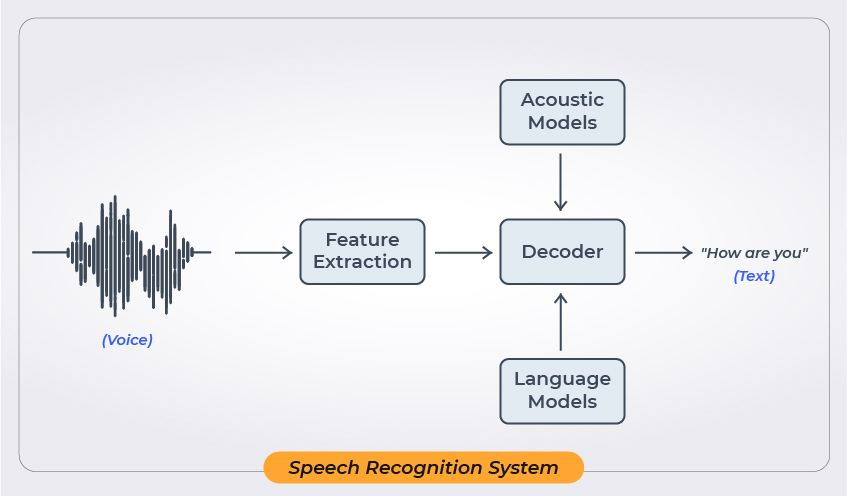
\includegraphics{spr.jpg}

\begin{center}\rule{0.5\linewidth}{\linethickness}\end{center}

\textbf{\emph{Machine Translation}}:

Machine Translation is the task of automatically translating one natural
language into another while retaining the meaning of the original text.

Each word from the source language is mapped to multiple candidate words
of the target language; the language model of the target language then
can rank the most likely sequence of candidate target words. This works
because more likely sentences are probably better translations.

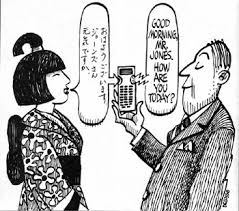
\includegraphics{mt_2.jpg}

For eg: Translating a sentence refering about employees who left, model
would probably state that
\texttt{P(former\ employee)\ \textgreater{}\ P(older\ employee)} as the
`older' might also refer to age of the employee and thus, not as
probable as `former'

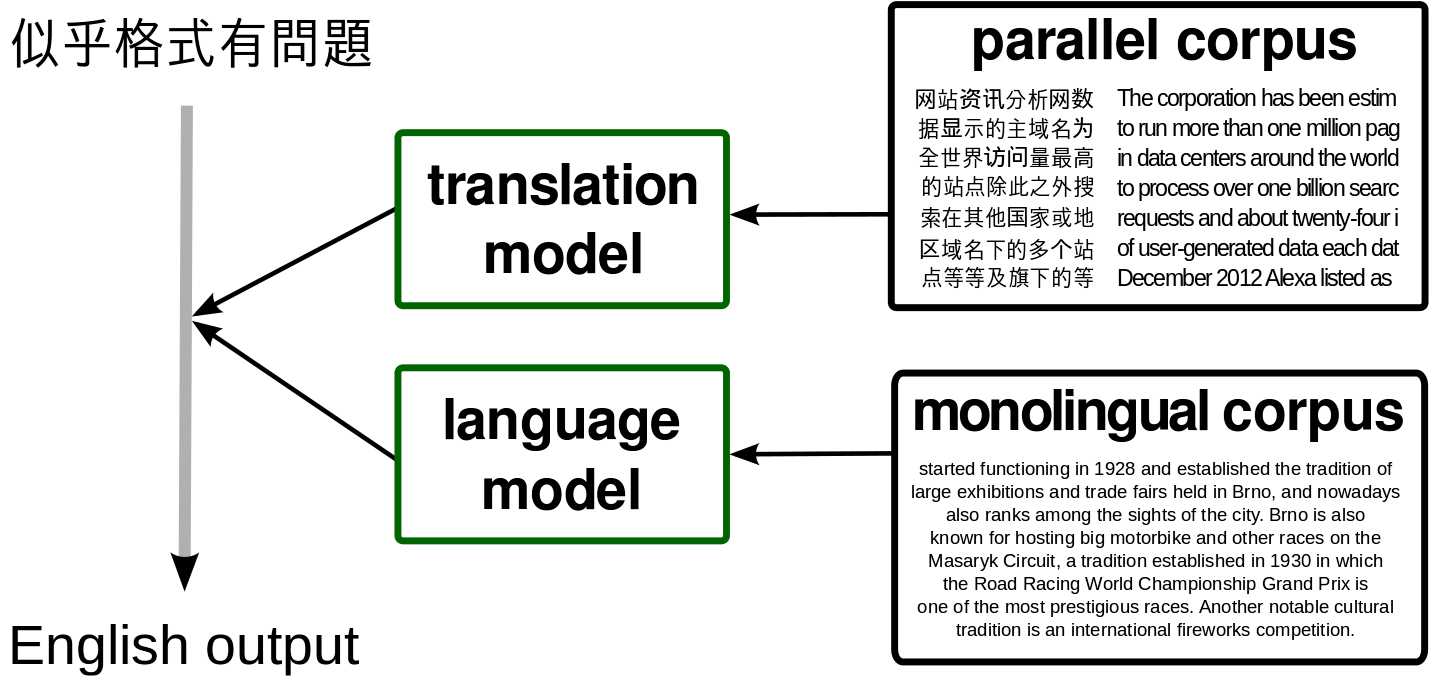
\includegraphics{mt.png}

\begin{center}\rule{0.5\linewidth}{\linethickness}\end{center}

\textbf{\emph{Spell checking}}:

The task of spellchecking involves checking for spelling errors and
possibly suggesting alternatives depending upon the context.

Spell checking is done by the machine when it observes a word which is
not recognized as a \texttt{known\ word} (i.e.~the word does not occur
in a list of known words). It then finds the closest known words to the
unknown words.

For eg: If someone writes \texttt{fomr}, the closest known words will be
\texttt{from} and \texttt{form}. These are the candidate corrections.
How can we select among these candidates the most likely correction for
the error \texttt{fomr}?

We then compare the Language Model probability of the sentences:

\begin{itemize}
\tightlist
\item
  \texttt{P(name\ into\ form)}
\item
  \texttt{P(name\ into\ from)}
\end{itemize}

and we hope that the right correction {[}name into form{]} will be
selected.

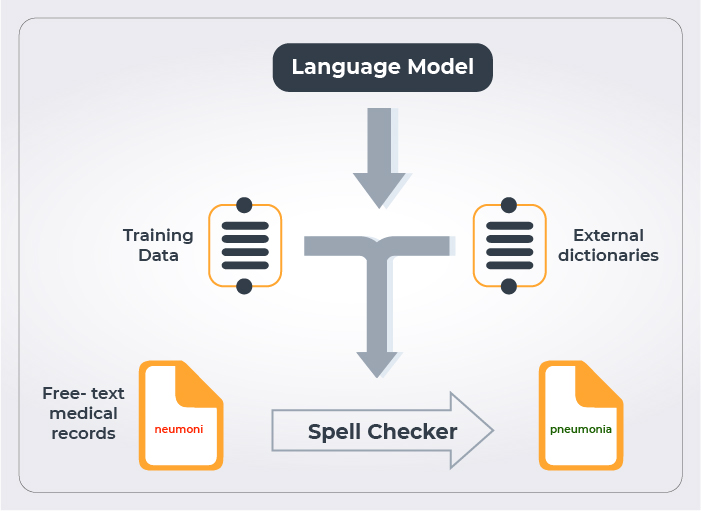
\includegraphics{lm.jpg}

\begin{center}\rule{0.5\linewidth}{\linethickness}\end{center}

Let's now see how we can go about creating a language model.

    \hypertarget{statistical-language-modeling}{%
\section{2. Statistical Language
Modeling}\label{statistical-language-modeling}}

Description: In this chapter, we will learn one of the most popular
method of modeling language i.e.~Statistical Language Modeling

    \hypertarget{n-grams}{%
\subsection{2.1 N-grams}\label{n-grams}}

    So we established that one way to model natural languagues is by
measuring the probability of sentences. So our aim is to get the
probability of a given sentence as being good, but before that let's
first focus on getting the probability of given word as being the next
word in a given sentence.

To build a language model, let's start with simple task of calculating
probability \(P(w|h)\), the probability of a word w given some history
h.

Suppose the history h is ``its lake is so clear that'' and we want to
know the probability that the next word w is ``the'':

\[ P (\text{the} | \text{its lake is so transparent that})\]

One of the ways to estimate this probability is from frequency counts.

Take a very large corpus(collection of written texts), count the number
of times ``its lake is so clear that'' is present, and then count the
number of times ``this'' is followed by ``the''.

This would be similar to answering the question ``Out of the times we
saw the history h, how many times was it followed by the word w''

So the probability will be calculated as:

\[ P(\text{the}|\text{its lake is so clear that}) = \frac{C(\text{its lake is so clear that the})}{C(\text{its lake is so clear that})} \]

With a large enough corpus(\textbf{\emph{which internet is}}), we can
compute these counts and estimate the probability from above equation.

While this method of estimating probabilities directly from counts is
intuitive and works fine in many cases, it turns out that even the web
isn't big enough to give us good estimates in most of the cases. That is
because as mentioned before, language is creative and new things emerge;
new sentences are created all the time, and we won't always be able to
count entire sentences. Even simple extensions of the example sentence
may have counts of 0 (such as ``Amsterdam's lake is so clear that
the'').

Additionally, if we wanted to know the probability(joint) of the entire
sequence of words(which is what a language model has to do) in `its lake
is so clear', the question we need to solve is ``out of all possible
sequences of five words, how many of them are `its lake is so clear'?''

Mathematically, joint probability for a n-word sentence will look
something like:

\[ \begin{align} P(w_1^n) &= P(w_1).P(w_2 | w_1).P(w_3 | w_1^2).P(w_4 | w_1^3) \dots\dots P(w_n | w_1^{n-1})\\ &= \prod_{k=1}^{n}P(w_k|w_1^{k-1}) \end{align} \]

We have to find probability of a word as being the next word with this
history among all the possible history.

Applying that to our sentence we will get

\[ \begin{align} P(\text{its lake  is  so  clear that the})\end{align}\]

\[\begin{align} = P(\text{its}).P(\text{lake} | \text{its}).P(\text{is}| \text{its lake}).P(\text{so}| \text{its lake is}).P(\text{clear}|\text{its lake is so}).P(\text{that}|\text{its lake is so clear}).P(\text{the}|\text{its lake is so clear that})......\end{align} \]

This seems a lot of work doesn't it?

Conclusion: We need better ways of estimating the probability of a word
w given a history h.

Construction of N-grams model is one of the solutions.

\textbf{What is N-grams?}

N-grams are the simplest type of tool available to construct a language
model.

An N-gram is a sequence of N words.

\emph{The intuition of the n-gram model is that instead of computing the
probability of a word given its entire history, we can
\textbf{approximate} the history by just the last few words.}

The bigram(2- grams) model, for example, approximates the probability of
a word w by using only the conditional probability of the preceding word
\(P(w_n |w_{n−1})\). Put in other way, instead of computing the
probability

\[P(\text{the}|\text{Amsterdam’s lake is so clear that})\]

we approximate it with just the probability:
\[P(\text{the}|\text{that})\]

Similar to bigram, we also have unigram(n=1), trigram(n=3), 4-grams and
so on.

Following is an image explaining the difference:

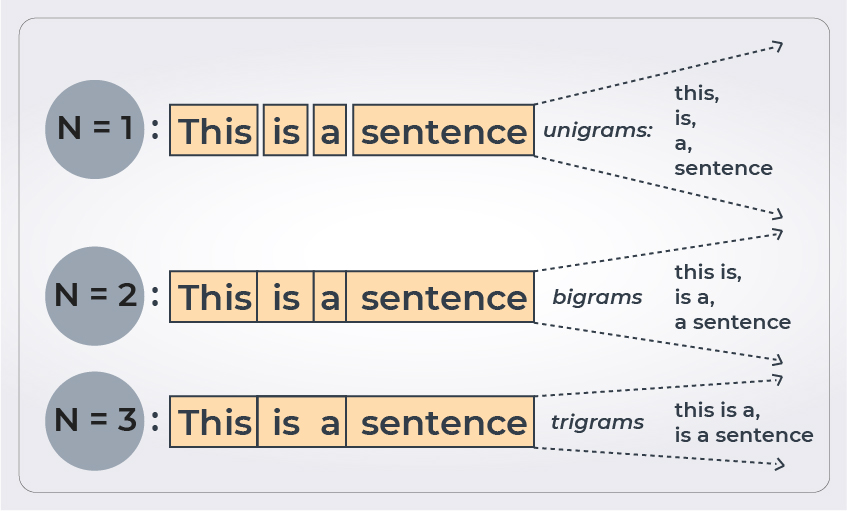
\includegraphics{ngram.jpg}

Let's try to understand n-grams better using an example.

Consider a corpus containing the following four sentences and we would
like to find the probability that ``You'' starts the sentence.

\(<s>\) You are a data scientist \(</s>\)

\(<s>\) Data scientist you are \(</s>\)

\(<s>\) You love statistics \(</s>\)

Here \(<s>\) and \(</s>\) denote the start and end of the sentence
respectively.

\textbf{Note:} We need \(<s>\) at the beginning of the sentence to get
the bigram context of the first word. Similarly, we need the end-symbol
\(</s>\) to get the bigram context of the last word.

Following will be the conditional probabilities of the words of corpus:

\begin{align}
& P(You|<s>) = \frac{2}{3} = .67  & \qquad &  P(Data|<s>) = \frac{1}{3} = .33  \\
& P(</s>|scientist) = \frac{1}{2} = .5  & \qquad &  P(</s>|are) = \frac{1}{2} = .5  \\
& P(</s>|statistics) = \frac{1}{1} = 1  & \qquad &  P(are|You) = \frac{2}{3} = .67  \\
& P(a|are) = \frac{1}{2} = .5  & \qquad &  P(data|a) = \frac{1}{1} = 1  \\
& P(scientist|data) = \frac{2}{2} = 1  & \qquad &  P(statistics|love) = \frac{1}{1}=1  \\
& P(love|you) = \frac{1}{3} = 0.33
\end{align}

Let's take the example of \(P(are|You)\) above. First we calculate all
possible bigrams in the corpus that is ``You are''. Then we calculate
all possible bigrams in corpus with You(or you) as its first word.

In the above corpus we have 2 instances of ``You are'' and 3 total
instances where you is first word in a bigram(``You are'' in first line,
``you are'' in second line and ``You love'' in third line).

Therefore \(P(are|You)=\frac{2}{3}\)

When we use a bigram model to predict the probability, we are making the
following approximation:
\[ P(w_n |w^{n−1}_1 ) \approx P(w_n |w_{n−1} ) \]

\textbf{Here \(w_n\) is the \(n_{th}\) word and \(w^{n−1}_1\) is
sequence of all n-1 words}

This assumption that the probability of a word depends only on the
previous word is called a Markov assumption

\textbf{Markov Assumption} *** A random process has the Markov property
if we can predict the probability of future states of the process
without looking at every event in the past i.e next step depends only
upon the present state and not on the sequence of events that preceded
it.

This helps in generalizing the bigram (which looks one word into the
past) to trigram (which looks two words into the past) and ultimately to
the n-gram (which looks n − 1 words into the past). ***

Markov assumption fits nicely with the n-gram model because of natural
language's underlying property that in most of the cases, the
probability of the word depends on its surrounding words.

Let's now look at how we can calculate probabilities of sentences.

    \hypertarget{task}{%
\section{Task}\label{task}}

\begin{itemize}
\item
  Test sentence tokens(Test sentence broken down to words) ,corpus and
  frequency counts(for unigram and bigram) is already given.(Print and
  see the values of the different values created)
\item
  Function definition of \texttt{get\_bigram\_probability()} with
  parameters \texttt{first},\texttt{second} is given.
\item
  Inside the function:

  \begin{itemize}
  \item
    Store the conditional frequency of the \texttt{first} and
    \texttt{second}
    term(\texttt{conditional\_freq{[}first{]}{[}second{]}}) in a
    variable called
    \texttt{\textquotesingle{}bigram\_freq\textquotesingle{}}.
  \item
    Store the frequency of the \texttt{first}
    term(\texttt{updated\_uni\_freq{[}first{]}}) in a variable called
    \texttt{\textquotesingle{}unigram\_freq\textquotesingle{}}.
  \item
    Return the value calculated by dividing
    \texttt{\textquotesingle{}bigram\_freq\textquotesingle{}} with
    \texttt{\textquotesingle{}unigram\_freq\textquotesingle{}}
  \end{itemize}
\item
  Create an empty list called
  \texttt{\textquotesingle{}prob\_list\textquotesingle{}}.
\item
  Create a variable called
  \texttt{\textquotesingle{}previous\textquotesingle{}} and save the
  string \texttt{\textquotesingle{}*start\_end*\textquotesingle{}} in
  it.(This will be our sentence beginner mark
  \texttt{\textless{}s\textgreater{}} that we encountered while learning
  bigram probabilities)
\item
  Run a loop \texttt{for\ token\ in\ test\_sentence\_tokens}. Inside the
  loop

  \begin{itemize}
  \tightlist
  \item
    Calculate the bigram probability by calling the function
    \texttt{"get\_bigram\_probability(previous,\ token)"} and store it
    in a variable called
    \texttt{\textquotesingle{}next\_probability\textquotesingle{}}
  \item
    Save the current \texttt{\textquotesingle{}token\textquotesingle{}}
    as \texttt{\textquotesingle{}previous\textquotesingle{}}
  \item
    Append
    \texttt{\textquotesingle{}next\_probability\textquotesingle{}} to
    \texttt{\textquotesingle{}prob\_list\textquotesingle{}}
  \end{itemize}
\end{itemize}

\textbf{Note:} Calculation of the final term is still left.

\begin{itemize}
\item
  Calculate the bigram prob. of the final term by calling the function
  \texttt{"get\_bigram\_probability()"} with
  \texttt{\textquotesingle{}previous\textquotesingle{}}(This will be
  store the final term after coming out of the loop) and
  \texttt{\textquotesingle{}*start\_end*\textquotesingle{}}.
\item
  Append the above calculated value to
  \texttt{\textquotesingle{}prob\_list\textquotesingle{}}
\end{itemize}

    \begin{Verbatim}[commandchars=\\\{\}]
{\color{incolor}In [{\color{incolor}1}]:} \PY{k+kn}{import} \PY{n+nn}{nltk}
        \PY{k+kn}{from} \PY{n+nn}{nltk}\PY{n+nn}{.}\PY{n+nn}{corpus} \PY{k}{import} \PY{n}{brown}
        
        \PY{c+c1}{\PYZsh{} Corpus}
        \PY{n}{words} \PY{o}{=} \PY{n}{brown}\PY{o}{.}\PY{n}{words}\PY{p}{(}\PY{p}{)}
        \PY{n}{words}\PY{o}{=}\PY{p}{[}\PY{n}{w}\PY{o}{.}\PY{n}{lower}\PY{p}{(}\PY{p}{)} \PY{k}{for} \PY{n}{w} \PY{o+ow}{in} \PY{n}{words}\PY{p}{]}
        
        \PY{c+c1}{\PYZsh{} Unigram frequency }
        \PY{n}{uni\PYZus{}freq} \PY{o}{=} \PY{n}{nltk}\PY{o}{.}\PY{n}{FreqDist}\PY{p}{(}\PY{n}{w}\PY{o}{.}\PY{n}{lower}\PY{p}{(}\PY{p}{)} \PY{k}{for} \PY{n}{w} \PY{o+ow}{in} \PY{n}{words}\PY{p}{)}
        
        \PY{c+c1}{\PYZsh{} Size of corpus}
        \PY{n}{total\PYZus{}words} \PY{o}{=} \PY{n+nb}{len}\PY{p}{(}\PY{n}{words}\PY{p}{)}
        
        \PY{n+nb}{print}\PY{p}{(}\PY{l+s+s1}{\PYZsq{}}\PY{l+s+s1}{Frequency of tokens of the sample sentence:}\PY{l+s+s1}{\PYZsq{}}\PY{p}{,}\PY{n}{total\PYZus{}words}\PY{p}{)}
        
        \PY{c+c1}{\PYZsh{}Sentence }
        \PY{n}{test\PYZus{}sentence\PYZus{}tokens}\PY{o}{=}\PY{p}{[}\PY{l+s+s1}{\PYZsq{}}\PY{l+s+s1}{this}\PY{l+s+s1}{\PYZsq{}}\PY{p}{,}\PY{l+s+s1}{\PYZsq{}}\PY{l+s+s1}{is}\PY{l+s+s1}{\PYZsq{}}\PY{p}{,}\PY{l+s+s1}{\PYZsq{}}\PY{l+s+s1}{a}\PY{l+s+s1}{\PYZsq{}}\PY{p}{,}\PY{l+s+s1}{\PYZsq{}}\PY{l+s+s1}{sunny}\PY{l+s+s1}{\PYZsq{}}\PY{p}{,}\PY{l+s+s1}{\PYZsq{}}\PY{l+s+s1}{day}\PY{l+s+s1}{\PYZsq{}}\PY{p}{,}\PY{l+s+s1}{\PYZsq{}}\PY{l+s+s1}{.}\PY{l+s+s1}{\PYZsq{}}\PY{p}{]}
        
        
        \PY{k}{for} \PY{n}{word} \PY{o+ow}{in} \PY{n}{test\PYZus{}sentence\PYZus{}tokens}\PY{p}{:}
            \PY{n+nb}{print}\PY{p}{(}\PY{l+s+s1}{\PYZsq{}}\PY{l+s+s1}{Frequency of }\PY{l+s+s1}{\PYZdq{}}\PY{l+s+s1}{\PYZsq{}}\PY{p}{,}\PY{n}{word}\PY{p}{,}\PY{l+s+s1}{\PYZsq{}}\PY{l+s+s1}{\PYZdq{}}\PY{l+s+s1}{ is }\PY{l+s+s1}{\PYZsq{}}\PY{p}{,}\PY{n}{uni\PYZus{}freq}\PY{p}{[}\PY{n}{word}\PY{p}{]}\PY{p}{)}
        
        \PY{n+nb}{print}\PY{p}{(}\PY{l+s+s1}{\PYZsq{}}\PY{l+s+se}{\PYZbs{}n}\PY{l+s+se}{\PYZbs{}n}\PY{l+s+s1}{\PYZsq{}}\PY{p}{)}
            
        \PY{c+c1}{\PYZsh{} Creating bigrams}
        
        \PY{n}{bigram\PYZus{}words} \PY{o}{=} \PY{p}{[}\PY{p}{]}
        \PY{n}{previous} \PY{o}{=} \PY{l+s+s1}{\PYZsq{}}\PY{l+s+s1}{EMPTY}\PY{l+s+s1}{\PYZsq{}}
        \PY{n}{sentences} \PY{o}{=} \PY{l+m+mi}{0}
        \PY{k}{for} \PY{n}{word} \PY{o+ow}{in} \PY{n}{words}\PY{p}{:}
            \PY{k}{if} \PY{n}{previous} \PY{o+ow}{in} \PY{p}{[}\PY{l+s+s1}{\PYZsq{}}\PY{l+s+s1}{EMPTY}\PY{l+s+s1}{\PYZsq{}}\PY{p}{,}\PY{l+s+s1}{\PYZsq{}}\PY{l+s+s1}{.}\PY{l+s+s1}{\PYZsq{}}\PY{p}{,}\PY{l+s+s1}{\PYZsq{}}\PY{l+s+s1}{?}\PY{l+s+s1}{\PYZsq{}}\PY{p}{,}\PY{l+s+s1}{\PYZsq{}}\PY{l+s+s1}{!}\PY{l+s+s1}{\PYZsq{}}\PY{p}{]}\PY{p}{:}
                \PY{c+c1}{\PYZsh{}\PYZsh{} insert word\PYZus{}boundaries at beginning of Brown,}
                \PY{n}{bigram\PYZus{}words}\PY{o}{.}\PY{n}{append}\PY{p}{(}\PY{l+s+s1}{\PYZsq{}}\PY{l+s+s1}{*start\PYZus{}end*}\PY{l+s+s1}{\PYZsq{}}\PY{p}{)}
            \PY{k}{else}\PY{p}{:}
                \PY{n}{bigram\PYZus{}words}\PY{o}{.}\PY{n}{append}\PY{p}{(}\PY{n}{word}\PY{p}{)}
            
            \PY{n}{previous} \PY{o}{=} \PY{n}{word}
        
        
            
            
        \PY{n}{bigram\PYZus{}words}\PY{o}{.}\PY{n}{append}\PY{p}{(}\PY{l+s+s1}{\PYZsq{}}\PY{l+s+s1}{*start\PYZus{}end*}\PY{l+s+s1}{\PYZsq{}}\PY{p}{)} \PY{c+c1}{\PYZsh{}\PYZsh{} assume one additional *start\PYZus{}end* at the end of Brown}
        
        \PY{n}{updated\PYZus{}uni\PYZus{}freq}  \PY{o}{=} \PY{n}{nltk}\PY{o}{.}\PY{n}{FreqDist}\PY{p}{(}\PY{n}{w}\PY{o}{.}\PY{n}{lower}\PY{p}{(}\PY{p}{)} \PY{k}{for} \PY{n}{w} \PY{o+ow}{in} \PY{n}{bigram\PYZus{}words}\PY{p}{)}
        
        
        \PY{n+nb}{print}\PY{p}{(}\PY{l+s+s1}{\PYZsq{}}\PY{l+s+s1}{Calculating bigram probalities for sentence, including bigrams with sentence boundaries, i.e., *start\PYZus{}end*}\PY{l+s+s1}{\PYZsq{}}\PY{p}{)}
        
        
        \PY{c+c1}{\PYZsh{} Bigram corpus}
        \PY{n}{bigrams} \PY{o}{=} \PY{n}{nltk}\PY{o}{.}\PY{n}{bigrams}\PY{p}{(}\PY{n}{w}\PY{o}{.}\PY{n}{lower}\PY{p}{(}\PY{p}{)} \PY{k}{for} \PY{n}{w} \PY{o+ow}{in} \PY{n}{bigram\PYZus{}words}\PY{p}{)}
        
        
        \PY{c+c1}{\PYZsh{} Bigram probabilities}
        \PY{n}{conditional\PYZus{}freq} \PY{o}{=} \PY{n}{nltk}\PY{o}{.}\PY{n}{ConditionalFreqDist}\PY{p}{(}\PY{n}{bigrams}\PY{p}{)}
        
        
        
        \PY{c+c1}{\PYZsh{} Code begins here}
        
        
        \PY{c+c1}{\PYZsh{} Function to calculate bigram probability}
        \PY{k}{def} \PY{n+nf}{get\PYZus{}bigram\PYZus{}probability}\PY{p}{(}\PY{n}{first}\PY{p}{,}\PY{n}{second}\PY{p}{)}\PY{p}{:}
            
            \PY{n}{bigram\PYZus{}freq} \PY{o}{=} \PY{n}{conditional\PYZus{}freq}\PY{p}{[}\PY{n}{first}\PY{p}{]}\PY{p}{[}\PY{n}{second}\PY{p}{]}
            \PY{n}{unigram\PYZus{}freq} \PY{o}{=} \PY{n}{updated\PYZus{}uni\PYZus{}freq}\PY{p}{[}\PY{n}{first}\PY{p}{]}
        
            \PY{n}{bigram\PYZus{}prob} \PY{o}{=} \PY{p}{(}\PY{n}{bigram\PYZus{}freq}\PY{p}{)}\PY{o}{/}\PY{p}{(}\PY{n}{unigram\PYZus{}freq}\PY{p}{)}
            
            \PY{k}{return} \PY{n}{bigram\PYZus{}prob}
        
        \PY{c+c1}{\PYZsh{}\PYZsh{} Calculating the bigram probability}
        
        \PY{n}{prob\PYZus{}list}\PY{o}{=}\PY{p}{[}\PY{p}{]}
        \PY{n}{previous} \PY{o}{=} \PY{l+s+s1}{\PYZsq{}}\PY{l+s+s1}{*start\PYZus{}end*}\PY{l+s+s1}{\PYZsq{}}
        
        \PY{k}{for} \PY{n}{token} \PY{o+ow}{in} \PY{n}{test\PYZus{}sentence\PYZus{}tokens}\PY{p}{:}
            \PY{n}{next\PYZus{}probability} \PY{o}{=} \PY{n}{get\PYZus{}bigram\PYZus{}probability}\PY{p}{(}\PY{n}{previous}\PY{p}{,}\PY{n}{token}\PY{p}{)}
            \PY{n+nb}{print}\PY{p}{(}\PY{n}{previous}\PY{p}{,}\PY{n}{token}\PY{p}{,}\PY{p}{(}\PY{n+nb}{float}\PY{p}{(}\PY{l+s+s1}{\PYZsq{}}\PY{l+s+si}{\PYZpc{}.3g}\PY{l+s+s1}{\PYZsq{}} \PY{o}{\PYZpc{}} \PY{n}{next\PYZus{}probability}\PY{p}{)}\PY{p}{)}\PY{p}{)}
            \PY{n}{previous} \PY{o}{=} \PY{n}{token}
            \PY{n}{prob\PYZus{}list}\PY{o}{.}\PY{n}{append}\PY{p}{(}\PY{n}{next\PYZus{}probability}\PY{p}{)}
        
        
            
        \PY{c+c1}{\PYZsh{} For the final term    }
        \PY{n}{next\PYZus{}probability} \PY{o}{=} \PY{n}{get\PYZus{}bigram\PYZus{}probability}\PY{p}{(}\PY{n}{previous}\PY{p}{,}\PY{l+s+s1}{\PYZsq{}}\PY{l+s+s1}{*start\PYZus{}end*}\PY{l+s+s1}{\PYZsq{}}\PY{p}{)}
        \PY{n+nb}{print}\PY{p}{(}\PY{n}{previous}\PY{p}{,}\PY{l+s+s1}{\PYZsq{}}\PY{l+s+s1}{*start\PYZus{}end*}\PY{l+s+s1}{\PYZsq{}}\PY{p}{,}\PY{n}{next\PYZus{}probability}\PY{p}{)}
        \PY{n}{prob\PYZus{}list}\PY{o}{.}\PY{n}{append}\PY{p}{(}\PY{n}{next\PYZus{}probability}\PY{p}{)}    
        
        \PY{c+c1}{\PYZsh{} print(prob\PYZus{}list)    }
\end{Verbatim}


    \begin{Verbatim}[commandchars=\\\{\}]
Frequency of tokens of the sample sentence: 1161192
Frequency of " this " is  5145
Frequency of " is " is  10109
Frequency of " a " is  23195
Frequency of " sunny " is  13
Frequency of " day " is  687
Frequency of " . " is  49346



Calculating bigram probalities for sentence, including bigrams with sentence boundaries, i.e., *start\_end*
*start\_end* this 0.0083
this is 0.0503
is a 0.0861
a sunny 4.51e-05
sunny day 0.154
day . 0.163
. *start\_end* 1.0

    \end{Verbatim}

    \hypertarget{hints}{%
\section{Hints}\label{hints}}

You can find the bigram probabilities by writing code similar to:

\begin{Shaded}
\begin{Highlighting}[]
\NormalTok{prob_list}\OperatorTok{=}\NormalTok{[]}
\NormalTok{previous }\OperatorTok{=} \StringTok{'*start_end*'}
\ControlFlowTok{for}\NormalTok{ token }\KeywordTok{in}\NormalTok{ test_sentence_tokens:}
\NormalTok{    next_probability }\OperatorTok{=}\NormalTok{ get_bigram_probability(previous,token)}
    \BuiltInTok{print}\NormalTok{(previous,token,(}\BuiltInTok{float}\NormalTok{(}\StringTok{'}\SpecialCharTok\NormalTok{ next_probability)))}
\NormalTok{    previous }\OperatorTok{=}\NormalTok{ token}
\NormalTok{    prob_list.append(next_probability)}

    
\CommentTok{# For the final term    }
\NormalTok{next_probability }\OperatorTok{=}\NormalTok{ get_bigram_probability(previous,}\StringTok{'*start_end*'}\NormalTok{)}
\BuiltInTok{print}\NormalTok{(previous,}\StringTok{'*start_end*'}\NormalTok{,next_probability)}
\NormalTok{prob_list.append(next_probability)    }

\BuiltInTok{print}\NormalTok{(prob_list)    }
\end{Highlighting}
\end{Shaded}

\hypertarget{test-cases}{%
\section{Test Cases}\label{test-cases}}

\#prob\_list

Variable declaration

round(prob\_list{[}1{]},2)==0.05

    \hypertarget{success-message}{%
\section{Success Message}\label{success-message}}

Congrats! You have successfully found out bigram probabilities of the
sentence tokens

    \hypertarget{language-model-using-n-gram}{%
\subsection{2.2 Language model using
n-gram}\label{language-model-using-n-gram}}

    In the previous topic, we constructed an N-gram model(bigram model in
our case) for words, how will we now obtain a complete language model on
the basis of this ?

Simple, we will calculate the \texttt{joint\ probability} by multiplying
the respective n-gram probabilites.

Applying that to our sentence(from the previous chapter) we see that the
following calculation:

\[ \begin{align} P(\text{its lake  is  so  clear that the})\end{align}\]

\[\begin{align} = P(\text{its}).P(\text{lake} | \text{its}).P(\text{is}| \text{its lake}).P(\text{so}| \text{its lake is}).P(\text{clear}|\text{its lake is so}).P(\text{that}|\text{its lake is so clear}).P(\text{the}|\text{its lake is so clear that})\end{align}..... \]

gets reduced to

\[ \begin{align} P(\text{its lake  is  so  clear that the})\end{align}\]
\[\begin{align} = P(\text{its}|P\text{<s>}).P(\text{lake} | \text{its}).P(\text{is}| \text{lake}).P(\text{so}| \text{is}).P(\text{clear}|\text{so}).P(\text{that}|\text{clear}).P(\text{the}|\text{that})\end{align}.... \]

\begin{center}\rule{0.5\linewidth}{\linethickness}\end{center}

\textbf{Deep Dive(Optional)}

\emph{Mathematical representation of how joint probability is
calculated:}

Joint-probability of n-word sentence is:

\[ \begin{align} P(w_1^n) &= P(w_1).P(w_2 | w_1).P(w_3 | w_1^2).P(w_4 | w_1^3) \dots\dots P(w_n | w_1^{n-1})\\
 &= \prod_{k=1}^{n}P(w_k|w_1^{k-1}) \end{align} \]

Using Markov's assumption, we know

\[ P(w_n |w^{n−1}_1 ) \approx P(w_n |w_{n−1} ) \]

That will help obtain the following approximation:

\begin{align} P(w_1^n) = \prod_{n=1}^{n}P(w_k|w_{k-1}) \end{align}

\begin{center}\rule{0.5\linewidth}{\linethickness}\end{center}

Let us now try to understand how language model work better using a
bigram example:

Given below is the count of random 8 words(out of 100 distinct words)
from a food delivery app(Also known as the unigram table)

\begin{longtable}[]{@{}llllllll@{}}
\toprule
i & want & to & eat & italian & food & lunch & breakfast\tabularnewline
\midrule
\endhead
2532 & 928 & 2419 & 746 & 158 & 1012 & 342 & 277\tabularnewline
\bottomrule
\end{longtable}

Following is the bigram table for the same words

\begin{longtable}[]{@{}lllllllll@{}}
\toprule
- & i & want & to & eat & italian & food & lunch & buy\tabularnewline
\midrule
\endhead
i & 6 & 818 & 0 & 9 & 0 & 0 & 0 & 2\tabularnewline
want & 2 & 0 & 608 & 1 & 6 & 7 & 6 & 1\tabularnewline
to & 2 & 0 & 4 & 685 & 2 & 0 & 6 & 211\tabularnewline
eat & 0 & 0 & 2 & 0 & 15 & 3 & 42 & 0\tabularnewline
italian & 1 & 0 & 0 & 0 & 0 & 82 & 1 & 0\tabularnewline
food & 14 & 0 & 15 & 0 & 1 & 5 & 0 & 0\tabularnewline
lunch & 2 & 0 & 0 & 0 & 0 & 0 & 0 & 1\tabularnewline
buy & 1 & 0 & 0 & 0 & 0 & 14 & 0 & 0\tabularnewline
\bottomrule
\end{longtable}

Here row word is the first word and column word is the second word.

For example ``i want'' bigram appears 818 times in the corpus, ``eat
italian'' bigram appears 15 times in the corpus.

You can make a lot of interesting observations when comparing unigram
table with the bigram.

For e.g.~Out of the 928 times the word \texttt{want} appears, 818 times
it appears after the word \texttt{I}.

After calculating the bigram probability(\(P(w_n |w_{n−1} )\)) we get
the following table

\begin{longtable}[]{@{}lllllllll@{}}
\toprule
- & i & want & to & eat & italian & food & lunch & buy\tabularnewline
\midrule
\endhead
i & 0.002 & 0.32 & 0 & 0.003 & 0 & 0 & 0 & 0.0007\tabularnewline
want & 0.002 & 0 & 0.65 & 0.001 & 0.006 & 0.007 & 0.006 &
0.001\tabularnewline
to & 0.0008 & 0 & 0.001 & 0.28 & 0.0008 & 0 & 0.002 &
0.08\tabularnewline
eat & 0 & 0 & 0.002 & 0 & 0.02 & 0.004 & 0.05 & 0\tabularnewline
italian & 0.006 & 0 & 0 & 0 & 0 & 0.51 & 0.006 & 0\tabularnewline
food & 0.01 & 0 & 0.01 & 0 & 0.0009 & 0.01 & 0 & 0\tabularnewline
lunch & 0.005 & 0 & 0 & 0 & 0 & 0 & 0 & 0.002\tabularnewline
breakfast & 0.004 & 0 & 0 & 0 & 0 & 0.05 & 0 & 0\tabularnewline
\bottomrule
\end{longtable}

To get the probabilities we divide each count value of our bigram table
with the unigram count of the first word of the
bigram.\textless{}\center\textgreater{}

 For eg: To get the bigram probability of ``eat italian'', we divide the
bigram count of ``eat italian'' which is 15 by the total no. of
times(unigram count), eat(first word of bigram) appears in the corpus
which is 746.

Therefore,
\[ \begin{align} P(\text{eat italian}) = \frac{15}{746}= 0.02\end{align}\]

Using the bigram probability table, we can now easily compute the
probability of sentences like \texttt{I\ want\ italian\ lunch} by simply
multiplying the appropriate bigram probabilities together, as follows:

\[\begin{align}
P(\text{<s> i want italian lunch </s>})
&= P(\text{i|<s>}).P(\text{want|i}).P(\text{italian|want}).P(\text{lunch|italian}).P(\text{</s>|lunch}) \\
&= .22 \times .32 \times .006 \times 0.006 \times 0.7 \\
&= 0.0000017
\end{align}
\]

\textbf{Note:} \(P(\text{i|<s>})\) and \(P(\text{</s>|lunch})\) were not
in the above bigram probability table but can be easily calculated from
the corpus in a similar way.

You can refresh about n-gram model by going through this video on
\href{https://www.youtube.com/watch?v=GiyMGBuu45w}{N-gram by Machine
Learning TV}

    \hypertarget{evaluating-lms-perplexity}{%
\subsection{2.3 Evaluating LMs:
Perplexity}\label{evaluating-lms-perplexity}}

    We just successfully constructed one language model using n-grams.

We now need an evaluation method to check how good it is(Especially
because we have taken the Markov assumption) from the ``actual''
probability of the sentences?

Therefore we need a measure to evaluate language models.Following are
the two popular ways:

\textbf{Extrinsic evaluation:} This is the best and most intuitive way
to evaluate a model . It involves testing different models in how much
they help the application

For e.g.~We want to evaluate the language model for a spell checker.
Thus, for spell checker, we can compare the performance of two language
models by running the spell checker twice, once with each language
model, and seeing which gives the more accurate correction.

Unfortunately, running big NLP systems end-to-end is an expensive form
of evaluation.

\textbf{Intrinsic evaluation}:

It would be convenient to have a method that can be used to quickly
evaluate potential improvements in a language model.

An intrinsic evaluation method is one that measures the quality of a
model independent of any application.

Just like most of the statistical models in data science field, the
probabilities of an n-gram model come from the corpus it is trained on,
known as the training set. We can then measure the performance of the
n-gram model by its performance on the unseen data also known as the
test set.

Whichever model assigns a higher probability to the sentences present in
the test set is a better model.

\emph{Q:} So should we just compare the raw probabilities of different
models to decide which model is intrinsically better?

\emph{A:} NO

The reason for it is that not all probability distributions are created
equal.

For eg:

There's a lot more uncertainty about the outcome of the word
\texttt{surprise} in a 1000 word article as compared to a novel.(Novel
has a bigger corpus than the Article)

Another reason is if two distributions have the same number of outcomes,
how likely those outcomes are also affects your uncertainty.

For eg: Given two 500 word essays written one on `Global Warming' and
`Formula F1 Race', you are a lot less uncertain about the word `Polar
Bears' on the first essay than you are in the second essay.

In practice we don't use raw probability as our metric for evaluating
language models, but a variant called \textbf{perplexity}.

Perplexity gives measures of complexity in a way that accounts for the
above two reasons.

The perplexity of a language model on a test set is the inverse
probability of the test set, normalized by the number of words.

For a test set \(W = w_1 w_2 \dots w_N ,\):

\[\begin{align} PP(W) &= {(P(w_1 w_2 \dots w_N))}^{-\frac{1}{N}}\\\end{align}\]
\[\begin{align}&= \sqrt[N]{\frac{1}{P(w_1 w_2 \dots w_N)}} \\\end{align}\]
\[\begin{align}&= \sqrt[N]{\prod_{i=1}^{N}\frac{1}{P(w_i|w_1 w_2 \dots w_{i-1})}}\\\end{align}\]

\[\begin{align}&\text{Replacing the perplexity with a n-gram model, say a bigram language model, we get :}\\\end{align}\]
\[\begin{align}PP(W) &= \sqrt[N]{\prod_{i=1}^{N}\frac{1}{P(w_i|w_{i-1})}}\\\end{align}\]

\textbf{Note:}

\begin{enumerate}
\def\labelenumi{\arabic{enumi}.}
\item
  The inverse in the formula means the higher the conditional
  probability of the word sequence, the lower the perplexity. Therefore,
  minimizing perplexity is equivalent to maximizing the test set
  probability of the language model.
\item
  The term 1/N where N is the number of words, helps normalize for the
  length of the probability by the number of words. This way the longer
  the sentence the less probable it will be.
\item
  Based on multiple experiments, it's observed that of all the n-gram
  models, trigram(n=3) models perform the best in predicting the `real'
  world probabilities
\end{enumerate}

You can have a better understanding about Evaluating language models by
going through the video on
\href{https://www.youtube.com/watch?v=BAN3NB_SNHY}{Evaluation and
Perplexity by André Ribeiro de Miranda}

\textbf{Evaluation problem}

Consider the following bigram table from the previous topic:

\begin{longtable}[]{@{}lllllllll@{}}
\toprule
- & i & want & to & eat & italian & food & lunch & buy\tabularnewline
\midrule
\endhead
i & 0.002 & 0.32 & 0 & 0.003 & 0 & 0 & 0 & 0.0007\tabularnewline
want & 0.002 & 0 & 0.65 & 0.001 & 0.006 & 0.007 & 0.006 &
0.001\tabularnewline
to & 0.0008 & 0 & 0.001 & 0.28 & 0.0008 & 0 & 0.002 &
0.08\tabularnewline
eat & 0 & 0 & 0.002 & 0 & 0.02 & 0.004 & 0.05 & 0\tabularnewline
italian & 0.006 & 0 & 0 & 0 & 0 & 0.51 & 0.006 & 0\tabularnewline
food & 0.01 & 0 & 0.01 & 0 & 0.0009 & 0.01 & 0 & 0\tabularnewline
lunch & 0.005 & 0 & 0 & 0 & 0 & 0 & 0 & 0.002\tabularnewline
breakfast & 0.004 & 0 & 0 & 0 & 0 & 0.05 & 0 & 0\tabularnewline
\bottomrule
\end{longtable}

In the table majority of the values are zero. A matrix selected from a
random set of 10 words would be even more sparse.

The model we have assumed so far suffers from two drastic problems:

\textbf{1. Sparsity}

For any n-gram that has occurred a sufficient no. of times, we might
have a good estimate of its probability. But because any test corpus is
limited, some perfectly acceptable word sequences are bound to be
missing from it.

Since there are a combinatorial no. of possible strings, many rare(but
not impossible) combinations never occur in training resulting in system
incorrectly assigning zero probability to many parameters

For eg: If the bank data training set has the following sentences(among
many others):

``he was denied the loan''

``he was denied the loan offer''

``loan was refused to him''

But suppose our test set had a phrase like

``loan was denied to him''

That sentence makes perfect sense but the \$ P(\text {to|denied}) \$
will be 0 resulting in the overall probability of the test sentence to
be equal to 0.

\textbf{2. Limited vocabulary}

We assume our model knows all the words in the vocabulary which is
rarely the case.

Consider the following sentences of news data training set:

``denied the rumours''

``denied the report''

``denied the allegations''

``denied the news''

But suppose our test set had a phrase like

``denied the speculations''

Even though the test phrase makes perfect sense, since ``speculations''
word was not in the training set, \$ P(\text {speculations|the})\$ will
be 0 resulting in the overall probability of the test sentence to be
equal to 0.

We could choose a vocabulary (word list) that is fixed in advance but in
doing so we are limiting our model immensely.

How do we solve the dual problem of limited words and limited sentence
combinations that are in train set but appear in a test set in an unseen
context?

To keep a language model from assigning zero probability to these unseen
events, we'll have to take a bit of probability from some more frequent
events and give it to the events we've never seen.

This modification is called smoothing.

Let's look at smoothing in detail in the next topic.

    \hypertarget{task}{%
\subsection{Task}\label{task}}

\begin{itemize}
\item
  \texttt{prob\_list\_1} contains the bigram probabilities of
  \texttt{this\ is\ a\ sunny\ day}.
\item
  Multiply all the values of
  \texttt{\textquotesingle{}prob\_list\_1\textquotesingle{}} to find the
  bigram model probability of the sentence and store the result in a
  variable called \texttt{total\_prob\_1}
\end{itemize}

\begin{center}\rule{0.5\linewidth}{\linethickness}\end{center}

Following is a sample code calculation of perplexity

\textbf{Input:}

\begin{Shaded}
\begin{Highlighting}[]

\NormalTok{prob_list}\OperatorTok{=}\NormalTok{[}\FloatTok{0.1}\NormalTok{, }\FloatTok{0.023}\NormalTok{ ,}\FloatTok{0.09}\NormalTok{]}


\NormalTok{perplexity}\OperatorTok{=}\DecValTok{1}

\CommentTok{# Calculating N}
\NormalTok{N}\OperatorTok{=}\BuiltInTok{len}\NormalTok{(prob_list)}\OperatorTok{-}\DecValTok{2}


\CommentTok{# Calculating the perplexity}
\ControlFlowTok{for}\NormalTok{ val }\KeywordTok{in}\NormalTok{ prob_list:}
\NormalTok{    perplexity }\OperatorTok{=}\NormalTok{ perplexity }\OperatorTok{*}\NormalTok{ (}\DecValTok{1}\OperatorTok{/}\NormalTok{val)}

\NormalTok{perplexity }\OperatorTok{=} \BuiltInTok{pow}\NormalTok{(perplexity, }\DecValTok{1}\OperatorTok{/}\BuiltInTok{float}\NormalTok{(N)) }

\BuiltInTok{print}\NormalTok{(}\StringTok{"Perplexity= :"}\NormalTok{,perplexity)}
\end{Highlighting}
\end{Shaded}

\textbf{Output:}

\begin{Shaded}
\begin{Highlighting}[]
\NormalTok{Perplexity}\OperatorTok{=}\NormalTok{ : }\FloatTok{69.5048046856916}
\end{Highlighting}
\end{Shaded}

\begin{center}\rule{0.5\linewidth}{\linethickness}\end{center}

\begin{itemize}
\item
  Calculate the perplexity of the values of
  \texttt{\textquotesingle{}prob\_list\_1\textquotesingle{}}(similar to
  the above code) and store the result in a variable called
  \texttt{\textquotesingle{}perplexity\_1\textquotesingle{}}.
\item
  \texttt{prob\_list\_2} contains the bigram probabilities of
  \texttt{this\ place\ is\ beautiful}.
\item
  Multiply all the values of
  \texttt{\textquotesingle{}prob\_list\_2\textquotesingle{}} to find the
  bigram model probability of the sentence and store the result in a
  variable called \texttt{total\_prob\_2}
\item
  Calculate the perplexity of the values of
  \texttt{\textquotesingle{}prob\_list\_2\textquotesingle{}}(similar to
  the above code) and store the result in a variable called
  \texttt{\textquotesingle{}perplexity\_2\textquotesingle{}}
\end{itemize}

\textbf{Things to ponder upon:}

\begin{itemize}
\item
  Which sentence has a lower perplexity?
\item
  Between perplexity and total probability, which metric gives a better
  intuitive understanding of more probable sentence?
\end{itemize}

    \begin{Verbatim}[commandchars=\\\{\}]
{\color{incolor}In [{\color{incolor}2}]:} \PY{n}{prob\PYZus{}list}\PY{o}{=}\PY{p}{[}\PY{l+m+mf}{0.1}\PY{p}{,} \PY{l+m+mf}{0.023} \PY{p}{,}\PY{l+m+mf}{0.09}\PY{p}{]}
        
        
        \PY{n}{perplexity}\PY{o}{=}\PY{l+m+mi}{1}
        
        \PY{c+c1}{\PYZsh{} Calculating N}
        \PY{n}{N}\PY{o}{=}\PY{n+nb}{len}\PY{p}{(}\PY{n}{prob\PYZus{}list}\PY{p}{)}\PY{o}{\PYZhy{}}\PY{l+m+mi}{1}
        
        
        \PY{c+c1}{\PYZsh{} Calculating the perplexity}
        \PY{k}{for} \PY{n}{val} \PY{o+ow}{in} \PY{n}{prob\PYZus{}list}\PY{p}{:}
            \PY{n}{perplexity} \PY{o}{=} \PY{n}{perplexity} \PY{o}{*} \PY{p}{(}\PY{l+m+mi}{1}\PY{o}{/}\PY{n}{val}\PY{p}{)}
        
        \PY{n}{perplexity} \PY{o}{=} \PY{n+nb}{pow}\PY{p}{(}\PY{n}{perplexity}\PY{p}{,} \PY{l+m+mi}{1}\PY{o}{/}\PY{n+nb}{float}\PY{p}{(}\PY{n}{N}\PY{p}{)}\PY{p}{)} 
        
        \PY{n+nb}{print}\PY{p}{(}\PY{l+s+s2}{\PYZdq{}}\PY{l+s+s2}{Perplexity= :}\PY{l+s+s2}{\PYZdq{}}\PY{p}{,}\PY{n}{perplexity}\PY{p}{)}
\end{Verbatim}


    \begin{Verbatim}[commandchars=\\\{\}]
Perplexity= : 69.5048046856916

    \end{Verbatim}

    \begin{Verbatim}[commandchars=\\\{\}]
{\color{incolor}In [{\color{incolor}1}]:} \PY{l+s+sd}{\PYZdq{}\PYZdq{}\PYZdq{}For the sentence: \PYZsq{}this is a sunny day\PYZsq{} \PYZdq{}\PYZdq{}\PYZdq{}} 
        \PY{n}{prob\PYZus{}list\PYZus{}1}\PY{o}{=}\PY{p}{[}\PY{l+m+mf}{0.008303975842979365}\PY{p}{,} \PY{l+m+mf}{0.05030826140567201}\PY{p}{,} \PY{l+m+mf}{0.08609535184632229}\PY{p}{,} \PY{l+m+mf}{4.5083630133898384e\PYZhy{}05}\PY{p}{,} \PY{l+m+mf}{0.15384615384615385}\PY{p}{]}
        
        
        
        \PY{n}{total\PYZus{}prob\PYZus{}1} \PY{o}{=} \PY{l+m+mi}{1}
        
        \PY{c+c1}{\PYZsh{} Multiplying all the values of the probability and storing it}
        \PY{k}{for} \PY{n}{val} \PY{o+ow}{in} \PY{n}{prob\PYZus{}list\PYZus{}1}\PY{p}{:}
            \PY{n}{total\PYZus{}prob\PYZus{}1} \PY{o}{*}\PY{o}{=} \PY{n}{val}
        
        
        \PY{n+nb}{print}\PY{p}{(}\PY{l+s+s2}{\PYZdq{}}\PY{l+s+s2}{For the sentence\PYZhy{} }\PY{l+s+s2}{\PYZsq{}}\PY{l+s+s2}{this is a sunny day}\PY{l+s+s2}{\PYZsq{}}\PY{l+s+s2}{\PYZdq{}}\PY{p}{)}
        \PY{n+nb}{print}\PY{p}{(}\PY{l+s+s2}{\PYZdq{}}\PY{l+s+s2}{Total probability:}\PY{l+s+s2}{\PYZdq{}}\PY{p}{,}\PY{n}{total\PYZus{}prob\PYZus{}1}\PY{p}{)}
        
        
        \PY{n}{perplexity\PYZus{}1}\PY{o}{=}\PY{l+m+mi}{1}
        
        \PY{c+c1}{\PYZsh{} Calculating N}
        \PY{n}{N}\PY{o}{=}\PY{n+nb}{len}\PY{p}{(}\PY{n}{prob\PYZus{}list\PYZus{}1}\PY{p}{)}\PY{o}{\PYZhy{}}\PY{l+m+mi}{1}
        
        
        \PY{c+c1}{\PYZsh{} Calculating the perplexity}
        \PY{k}{for} \PY{n}{val} \PY{o+ow}{in} \PY{n}{prob\PYZus{}list\PYZus{}1}\PY{p}{:}
            \PY{n}{perplexity\PYZus{}1} \PY{o}{=} \PY{n}{perplexity\PYZus{}1} \PY{o}{*} \PY{p}{(}\PY{l+m+mi}{1}\PY{o}{/}\PY{n}{val}\PY{p}{)}
        
        \PY{n}{perplexity\PYZus{}1} \PY{o}{=} \PY{n+nb}{pow}\PY{p}{(}\PY{n}{perplexity\PYZus{}1}\PY{p}{,} \PY{l+m+mi}{1}\PY{o}{/}\PY{n+nb}{float}\PY{p}{(}\PY{n}{N}\PY{p}{)}\PY{p}{)} 
        
        \PY{n+nb}{print}\PY{p}{(}\PY{l+s+s2}{\PYZdq{}}\PY{l+s+s2}{Perplexity:}\PY{l+s+s2}{\PYZdq{}}\PY{p}{,}\PY{n}{perplexity\PYZus{}1}\PY{p}{)}
        
        
        
        \PY{l+s+sd}{\PYZdq{}\PYZdq{}\PYZdq{}For the sentence: \PYZsq{}this place is beautiful\PYZsq{} \PYZdq{}\PYZdq{}\PYZdq{}}
        \PY{n}{prob\PYZus{}list\PYZus{}2}\PY{o}{=}\PY{p}{[}\PY{l+m+mf}{0.008303975842979365}\PY{p}{,} \PY{l+m+mf}{0.0022194821208384712}\PY{p}{,} \PY{l+m+mf}{0.02185792349726776}\PY{p}{,} \PY{l+m+mf}{9.953219866626854e\PYZhy{}05}\PY{p}{]}
        
        \PY{n}{total\PYZus{}prob\PYZus{}2} \PY{o}{=} \PY{l+m+mi}{1}
        
        \PY{c+c1}{\PYZsh{} Multiplying all the values of the probability and storing it}
        \PY{k}{for} \PY{n}{val} \PY{o+ow}{in} \PY{n}{prob\PYZus{}list\PYZus{}2}\PY{p}{:}
            \PY{n}{total\PYZus{}prob\PYZus{}2} \PY{o}{*}\PY{o}{=} \PY{n}{val}
        
        \PY{n+nb}{print}\PY{p}{(}\PY{l+s+s2}{\PYZdq{}}\PY{l+s+se}{\PYZbs{}n}\PY{l+s+se}{\PYZbs{}n}\PY{l+s+s2}{For the sentence\PYZhy{} }\PY{l+s+s2}{\PYZsq{}}\PY{l+s+s2}{this place is beautiful}\PY{l+s+s2}{\PYZsq{}}\PY{l+s+s2}{\PYZdq{}}\PY{p}{)}    
        \PY{n+nb}{print}\PY{p}{(}\PY{l+s+s2}{\PYZdq{}}\PY{l+s+s2}{Total probability: }\PY{l+s+s2}{\PYZdq{}}\PY{p}{,}\PY{n}{total\PYZus{}prob\PYZus{}2}\PY{p}{)}
        
        
        \PY{n}{perplexity\PYZus{}2}\PY{o}{=}\PY{l+m+mi}{1}
        
        \PY{c+c1}{\PYZsh{} Calculating N}
        \PY{n}{N}\PY{o}{=}\PY{n+nb}{len}\PY{p}{(}\PY{n}{prob\PYZus{}list\PYZus{}2}\PY{p}{)}\PY{o}{\PYZhy{}}\PY{l+m+mi}{1}
        
        \PY{c+c1}{\PYZsh{} Calculating perplexity}
        \PY{k}{for} \PY{n}{val} \PY{o+ow}{in} \PY{n}{prob\PYZus{}list\PYZus{}2}\PY{p}{:}
            \PY{n}{perplexity\PYZus{}2} \PY{o}{=} \PY{n}{perplexity\PYZus{}2} \PY{o}{*} \PY{p}{(}\PY{l+m+mi}{1}\PY{o}{/}\PY{n}{val}\PY{p}{)}
        
        \PY{n}{perplexity\PYZus{}2} \PY{o}{=} \PY{n+nb}{pow}\PY{p}{(}\PY{n}{perplexity\PYZus{}2}\PY{p}{,} \PY{l+m+mi}{1}\PY{o}{/}\PY{n+nb}{float}\PY{p}{(}\PY{n}{N}\PY{p}{)}\PY{p}{)} 
        
        \PY{n+nb}{print}\PY{p}{(}\PY{l+s+s2}{\PYZdq{}}\PY{l+s+s2}{Perplexity: }\PY{l+s+s2}{\PYZdq{}}\PY{p}{,}\PY{n}{perplexity\PYZus{}2}\PY{p}{)}
\end{Verbatim}


    \begin{Verbatim}[commandchars=\\\{\}]
For the sentence- 'this is a sunny day'
Total probability: 2.494655687321879e-10
Perplexity: 251.62126814544143


For the sentence- 'this place is beautiful'
Total probability:  4.009684736463708e-11
Perplexity:  2921.6616783932823

    \end{Verbatim}

    \hypertarget{hints}{%
\section{Hints}\label{hints}}

You can find perplexity of sentence 1 by writing code similar to:

\begin{Shaded}
\begin{Highlighting}[]
\ControlFlowTok{for}\NormalTok{ val }\KeywordTok{in}\NormalTok{ prob_list_1:}
\NormalTok{    perplexity_1 }\OperatorTok{=}\NormalTok{ perplexity_1 }\OperatorTok{*}\NormalTok{ (}\DecValTok{1}\OperatorTok{/}\NormalTok{val)}

\NormalTok{perplexity_1 }\OperatorTok{=} \BuiltInTok{pow}\NormalTok{(perplexity_1, }\DecValTok{1}\OperatorTok{/}\BuiltInTok{float}\NormalTok{(N)) }
\end{Highlighting}
\end{Shaded}

Similarly, you can find perplexity of the other sentence.

\hypertarget{test-cases}{%
\section{Test Cases}\label{test-cases}}

\#total\_prob\_1 Variable declaration round(total\_prob\_1,10)==2e-10

\#perplexity\_1 Variable declaration round(perplexity\_1,2)==251.62

\#total\_prob\_2 Variable declaration round(total\_prob\_2,11)==4e-11

\#perplexity\_2 Variable declaration round(perplexity\_2,2)==2921.66

    \hypertarget{success-message}{%
\section{Success Message}\label{success-message}}

Congrats! You have successfully found the perplexity and total
probabilities of the given sentences!

    \hypertarget{smoothing}{%
\section{3. Smoothing}\label{smoothing}}

Description: In this chapter, we will learn the different types of
Smoothing that can be done

    \hypertarget{add-k-smoothing}{%
\subsection{3.1 Add-K Smoothing}\label{add-k-smoothing}}

    We just understood that to keep a language model from assigning zero
probability to these unseen events, we could take a bit of probability
from some more frequent events and give it to the events we've never
seen by a method called smoothing.

Following are some of the popular smoothing techniques:

\begin{itemize}
\item
  Laplace Smoothing/Add-K smoothing
\item
  Interpolation
\item
  Backoff
\end{itemize}

Let's try to understand them one by one.

\textbf{Laplace Smoothing}

The simplest way to do smoothing would be to add one to all the
bigram(or any n-gram) counts, before we normalize them into
probabilities. All the counts that used to be 0 will now have a count of
1, the counts of 1 will be 2, and so on and so forth.

This kind of smoothing is called Laplace smoothing.

Let's start with the application of Laplace smoothing to unigram(single
word) probabilities.

Mathematically If unsmoothed unigram probability of the word \(w_i\) is
its count \(c_i\) normalized by the total number of word tokens \(N\):

\[P(w_i) = \frac{c_i}{N}\]

Laplace smoothing merely adds one to each count (Its also called
one-smoothing). If there are V words in the vocabulary and each one is
incremented, we also need to adjust the denominator to take into account
the extra V observations.

\[P_{Laplace}(w_i) = \frac{c_i + 1}{N + V}\]

Let us try to understand Laplace smoothing of bigrams with the previous
food delivery app example.

Following is the original bigram count table

\begin{longtable}[]{@{}lllllllll@{}}
\toprule
- & i & want & to & eat & italian & food & lunch & buy\tabularnewline
\midrule
\endhead
i & 6 & 818 & 0 & 9 & 0 & 0 & 0 & 2\tabularnewline
want & 2 & 0 & 608 & 1 & 6 & 7 & 6 & 1\tabularnewline
to & 2 & 0 & 4 & 685 & 2 & 0 & 6 & 211\tabularnewline
eat & 0 & 0 & 2 & 0 & 15 & 3 & 42 & 0\tabularnewline
italian & 1 & 0 & 0 & 0 & 0 & 82 & 1 & 0\tabularnewline
food & 14 & 0 & 15 & 0 & 1 & 5 & 0 & 0\tabularnewline
lunch & 2 & 0 & 0 & 0 & 0 & 0 & 0 & 1\tabularnewline
buy & 1 & 0 & 0 & 0 & 0 & 14 & 0 & 0\tabularnewline
\bottomrule
\end{longtable}

After Laplace smoothing, the table transforms to

\begin{longtable}[]{@{}lllllllll@{}}
\toprule
- & i & want & to & eat & italian & food & lunch & buy\tabularnewline
\midrule
\endhead
i & 7 & 819 & 1 & 10 & 1 & 1 & 1 & 3\tabularnewline
want & 3 & 1 & 609 & 2 & 7 & 8 & 7 & 2\tabularnewline
to & 3 & 1 & 5 & 686 & 3 & 1 & 7 & 212\tabularnewline
eat & 1 & 1 & 3 & 1 & 16 & 4 & 43 & 1\tabularnewline
italian & 2 & 1 & 1 & 1 & 1 & 83 & 2 & 1\tabularnewline
food & 15 & 1 & 16 & 1 & 2 & 6 & 1 & 1\tabularnewline
lunch & 3 & 1 & 1 & 1 & 1 & 1 & 1 & 2\tabularnewline
buy & 2 & 1 & 1 & 1 & 1 & 15 & 1 & 1\tabularnewline
\bottomrule
\end{longtable}

We know that normal bigram probabilities are computed using the
following: \[ P(w_n|w_{n-1}) = \frac{C(w_{n-1}w_n)}{C(w_{n-1})} \]

This resulted in the following bigram probability table:

\begin{longtable}[]{@{}lllllllll@{}}
\toprule
- & i & want & to & eat & italian & food & lunch & buy\tabularnewline
\midrule
\endhead
i & 0.002 & 0.32 & 0 & 0.003 & 0 & 0 & 0 & 0.0007\tabularnewline
want & 0.002 & 0 & 0.65 & 0.001 & 0.006 & 0.007 & 0.006 &
0.001\tabularnewline
to & 0.0008 & 0 & 0.001 & 0.28 & 0.0008 & 0 & 0.002 &
0.08\tabularnewline
eat & 0 & 0 & 0.002 & 0 & 0.02 & 0.004 & 0.05 & 0\tabularnewline
italian & 0.006 & 0 & 0 & 0 & 0 & 0.51 & 0.006 & 0\tabularnewline
food & 0.01 & 0 & 0.01 & 0 & 0.0009 & 0.01 & 0 & 0\tabularnewline
lunch & 0.005 & 0 & 0 & 0 & 0 & 0 & 0 & 0.002\tabularnewline
breakfast & 0.004 & 0 & 0 & 0 & 0 & 0.05 & 0 & 0\tabularnewline
\bottomrule
\end{longtable}

For add-one smoothed bigram counts, we just need to normalize the
unigram count(denominator) by the number of distinct words V(in this
case V=100) in the vocabulary:
\[ P^*_{Laplace}(w_n|w_{n-1}) = \frac{C(w_{n-1}w_n) + 1}{C(w_{n-1}) + V} \]

This will result in the following bigram probability table

\begin{longtable}[]{@{}lllllllll@{}}
\toprule
- & i & want & to & eat & italian & food & lunch & buy\tabularnewline
\midrule
\endhead
i & 0.002 & 0.31 & 0.0003 & 0.003 & 0.0003 & 0.0003 & 0.0003 &
0.001\tabularnewline
want & 0.002 & 0.0009 & 0.59 & 0.001 & 0.006 & 0.007 & 0.006 &
0.001\tabularnewline
to & 0.001 & 0.0003 & 0.001 & 0.27 & 0.001 & 0.0003 & 0.002 &
0.08\tabularnewline
eat & 0.001 & 0.001 & 0.003 & 0.001 & 0.01 & 0.004 & 0.05 &
0.001\tabularnewline
italian & 0.007 & 0.003 & 0.003 & 0.003 & 0.003 & 0.32 & 0.007 &
0.003\tabularnewline
food & 0.01 & 0.0008 & 0.01 & 0.0008 & 0.001 & 0.005 & 0.0008 &
0.0008\tabularnewline
lunch & 0.006 & 0.002 & 0.002 & 0.002 & 0.002 & 0.002 & 0.002 &
0.004\tabularnewline
breakfast & 0.005 & 0.002 & 0.002 & 0.002 & 0.002 & 0.03 & 0.002 &
0.002\tabularnewline
\bottomrule
\end{longtable}

You can see that 0 probabilities have been converted to some non zero
value and at the same time, the value of earlier non zero probabilities
has also reduced for overall probability distribution(For e.g.
\(P(\text{to|want}\)) changed from 0.65 to 0.59)

The sharp change in probabilities occur because too much probability
mass is moved to all the zeros

Let's calculate the probability of the sentence ``i want italian lunch''
again

\[\begin{align}
P(\text{<s> i want italian lunch </s>})
&= P(\text{i|<s>}).P(\text{want|i}).P(\text{italian|want}).P(\text{lunch|italian}).P(\text{</s>|lunch}) \\
&= .22 \times .31 \times .006 \times 0.007 \times 0.7 \\
&= 0.000002
\end{align}\]

Though a practical smoothing algorithm for tasks like text
classification, unfortunately, Laplace smoothing doesn't perform well
for n-gram models.

\textbf{Add-K Smoothing}

One way to move a bit less of the \texttt{probability\ mass} from the
seen to the unseen events is instead of adding \texttt{1} to each count,
we just add a fractional count \texttt{k} (.5? .02?).

This modified add-1(Laplace) smoothing is called add-k smoothing.

Here instead of incrementing count by 1 we increment count by a
fractional value, helping us transfer a lesser amount of probability
from seen values of corpus to the unseen values of corpus.

Mathematical formula of finding probabilities after add-k smoothing is

\[ P^*_{add-k}(w_n|w_{n-1}) = \frac{C(w_{n-1}w_n) + k}{C(w_{n-1}) + kV} \]

There are multiple methods for selecting the optimum k value. For
example, by optimizing it on the testset.

Though better than Add-1 smoothing, Add-k smoothing still doesn't work
well for language modeling often leading to poor variance

Let's look at some other alternatives

    \hypertarget{task}{%
\section{TASK}\label{task}}

\begin{itemize}
\item
  The working code for the first task you completed is given with a new
  sentence \texttt{sunset\ looks\ magnificient.}
\item
  Run the code once as it is.
\end{itemize}

\textbf{We get an error of \texttt{division\ by\ 0} because magnificient
is not in our corpus.}

\textbf{Let's resolve that using Laplace Smoothing}

\begin{itemize}
\item
  Calculate Vocabulary of the corpus by finding the no. of unique words
  in the list \texttt{\textquotesingle{}words\textquotesingle{}} and
  save the the count in a variable called
  \texttt{\textquotesingle{}V\textquotesingle{}}
\item
  Inside the function: -Update the calculation of the term
  \texttt{\textquotesingle{}bigram\_prob\textquotesingle{}} by adding
  \texttt{1} to
  \texttt{\textquotesingle{}bigram\_freq\textquotesingle{}} and
  \texttt{V} to
  \texttt{\textquotesingle{}unigram\_freq\textquotesingle{}}
\item
  Multiply all the values of
  \texttt{\textquotesingle{}prob\_list\textquotesingle{}} to find the
  bigram model probability of the sentence and store the result in a
  variable called \texttt{total\_prob}
\end{itemize}

    \begin{Verbatim}[commandchars=\\\{\}]
{\color{incolor}In [{\color{incolor}3}]:} \PY{k+kn}{import} \PY{n+nn}{nltk}
        \PY{k+kn}{from} \PY{n+nn}{nltk}\PY{n+nn}{.}\PY{n+nn}{corpus} \PY{k}{import} \PY{n}{brown}
        
        
        
        \PY{k+kn}{import} \PY{n+nn}{nltk}
        \PY{k+kn}{from} \PY{n+nn}{nltk}\PY{n+nn}{.}\PY{n+nn}{corpus} \PY{k}{import} \PY{n}{brown}
        
        \PY{c+c1}{\PYZsh{} Corpus}
        \PY{n}{words} \PY{o}{=} \PY{n}{brown}\PY{o}{.}\PY{n}{words}\PY{p}{(}\PY{p}{)}
        \PY{n}{words}\PY{o}{=}\PY{p}{[}\PY{n}{w}\PY{o}{.}\PY{n}{lower}\PY{p}{(}\PY{p}{)} \PY{k}{for} \PY{n}{w} \PY{o+ow}{in} \PY{n}{words}\PY{p}{]}
        
        \PY{c+c1}{\PYZsh{} Unigram frequency }
        \PY{n}{uni\PYZus{}freq} \PY{o}{=} \PY{n}{nltk}\PY{o}{.}\PY{n}{FreqDist}\PY{p}{(}\PY{n}{w}\PY{o}{.}\PY{n}{lower}\PY{p}{(}\PY{p}{)} \PY{k}{for} \PY{n}{w} \PY{o+ow}{in} \PY{n}{words}\PY{p}{)}
        
        \PY{c+c1}{\PYZsh{} Size of corpus}
        \PY{n}{total\PYZus{}words} \PY{o}{=} \PY{n+nb}{len}\PY{p}{(}\PY{n}{words}\PY{p}{)}
        
        \PY{n+nb}{print}\PY{p}{(}\PY{l+s+s1}{\PYZsq{}}\PY{l+s+s1}{Frequency of tokens of the sample sentence:}\PY{l+s+s1}{\PYZsq{}}\PY{p}{)}
        
        \PY{k}{for} \PY{n}{word} \PY{o+ow}{in} \PY{n}{test\PYZus{}sentence\PYZus{}tokens}\PY{p}{:}
            \PY{n+nb}{print}\PY{p}{(}\PY{n}{word}\PY{p}{,}\PY{n}{uni\PYZus{}freq}\PY{p}{[}\PY{n}{word}\PY{p}{]}\PY{p}{)}
        
            
        \PY{c+c1}{\PYZsh{} Creating bigrams}
        
        \PY{n}{bigram\PYZus{}words} \PY{o}{=} \PY{p}{[}\PY{p}{]}
        \PY{n}{previous} \PY{o}{=} \PY{l+s+s1}{\PYZsq{}}\PY{l+s+s1}{EMPTY}\PY{l+s+s1}{\PYZsq{}}
        \PY{n}{sentences} \PY{o}{=} \PY{l+m+mi}{0}
        \PY{k}{for} \PY{n}{word} \PY{o+ow}{in} \PY{n}{words}\PY{p}{:}
            \PY{k}{if} \PY{n}{previous} \PY{o+ow}{in} \PY{p}{[}\PY{l+s+s1}{\PYZsq{}}\PY{l+s+s1}{EMPTY}\PY{l+s+s1}{\PYZsq{}}\PY{p}{,}\PY{l+s+s1}{\PYZsq{}}\PY{l+s+s1}{.}\PY{l+s+s1}{\PYZsq{}}\PY{p}{,}\PY{l+s+s1}{\PYZsq{}}\PY{l+s+s1}{?}\PY{l+s+s1}{\PYZsq{}}\PY{p}{,}\PY{l+s+s1}{\PYZsq{}}\PY{l+s+s1}{!}\PY{l+s+s1}{\PYZsq{}}\PY{p}{]}\PY{p}{:}
                \PY{c+c1}{\PYZsh{}\PYZsh{} insert word\PYZus{}boundaries at beginning of Brown,}
                \PY{n}{bigram\PYZus{}words}\PY{o}{.}\PY{n}{append}\PY{p}{(}\PY{l+s+s1}{\PYZsq{}}\PY{l+s+s1}{*start\PYZus{}end*}\PY{l+s+s1}{\PYZsq{}}\PY{p}{)}
            \PY{k}{else}\PY{p}{:}
                \PY{n}{bigram\PYZus{}words}\PY{o}{.}\PY{n}{append}\PY{p}{(}\PY{n}{word}\PY{p}{)}
            
            \PY{n}{previous} \PY{o}{=} \PY{n}{word}
        
        
            
            
        \PY{n}{bigram\PYZus{}words}\PY{o}{.}\PY{n}{append}\PY{p}{(}\PY{l+s+s1}{\PYZsq{}}\PY{l+s+s1}{*start\PYZus{}end*}\PY{l+s+s1}{\PYZsq{}}\PY{p}{)} \PY{c+c1}{\PYZsh{}\PYZsh{} assume one additional *start\PYZus{}end* at the end of Brown}
        
        \PY{n}{updated\PYZus{}uni\PYZus{}freq}  \PY{o}{=} \PY{n}{nltk}\PY{o}{.}\PY{n}{FreqDist}\PY{p}{(}\PY{n}{w}\PY{o}{.}\PY{n}{lower}\PY{p}{(}\PY{p}{)} \PY{k}{for} \PY{n}{w} \PY{o+ow}{in} \PY{n}{bigram\PYZus{}words}\PY{p}{)}
        
        
        \PY{n+nb}{print}\PY{p}{(}\PY{l+s+s1}{\PYZsq{}}\PY{l+s+se}{\PYZbs{}n}\PY{l+s+s1}{Calculating bigram counts for sentence, including bigrams with sentence boundaries, i.e., *BEGIN* and *END*}\PY{l+s+s1}{\PYZsq{}}\PY{p}{)}
        
        
        \PY{c+c1}{\PYZsh{} Bigram corpus}
        \PY{n}{bigrams} \PY{o}{=} \PY{n}{nltk}\PY{o}{.}\PY{n}{bigrams}\PY{p}{(}\PY{n}{w}\PY{o}{.}\PY{n}{lower}\PY{p}{(}\PY{p}{)} \PY{k}{for} \PY{n}{w} \PY{o+ow}{in} \PY{n}{bigram\PYZus{}words}\PY{p}{)}
        
        
        \PY{c+c1}{\PYZsh{} Bigram probabilities}
        \PY{n}{conditional\PYZus{}freq} \PY{o}{=} \PY{n}{nltk}\PY{o}{.}\PY{n}{ConditionalFreqDist}\PY{p}{(}\PY{n}{bigrams}\PY{p}{)}
        
        \PY{c+c1}{\PYZsh{}Sentence }
        \PY{n}{test\PYZus{}sentence\PYZus{}tokens}\PY{o}{=}\PY{p}{[}\PY{l+s+s1}{\PYZsq{}}\PY{l+s+s1}{sunset}\PY{l+s+s1}{\PYZsq{}}\PY{p}{,}\PY{l+s+s1}{\PYZsq{}}\PY{l+s+s1}{looks}\PY{l+s+s1}{\PYZsq{}}\PY{p}{,}\PY{l+s+s1}{\PYZsq{}}\PY{l+s+s1}{magnificient}\PY{l+s+s1}{\PYZsq{}}\PY{p}{,}\PY{l+s+s1}{\PYZsq{}}\PY{l+s+s1}{.}\PY{l+s+s1}{\PYZsq{}}\PY{p}{]}
        
        \PY{c+c1}{\PYZsh{} Code begins here}
        
        
        
        \PY{n}{V}\PY{o}{=}\PY{n+nb}{len}\PY{p}{(}\PY{n+nb}{set}\PY{p}{(}\PY{n}{words}\PY{p}{)}\PY{p}{)}
        
        
        \PY{c+c1}{\PYZsh{} Function to calculate bigram probability}
        \PY{k}{def} \PY{n+nf}{get\PYZus{}bigram\PYZus{}probability}\PY{p}{(}\PY{n}{first}\PY{p}{,}\PY{n}{second}\PY{p}{)}\PY{p}{:}
            
            \PY{n}{bigram\PYZus{}freq} \PY{o}{=} \PY{n}{conditional\PYZus{}freq}\PY{p}{[}\PY{n}{first}\PY{p}{]}\PY{p}{[}\PY{n}{second}\PY{p}{]}
            \PY{n}{unigram\PYZus{}freq} \PY{o}{=} \PY{n}{updated\PYZus{}uni\PYZus{}freq}\PY{p}{[}\PY{n}{first}\PY{p}{]}
        
            \PY{n}{bigram\PYZus{}prob} \PY{o}{=} \PY{p}{(}\PY{n}{bigram\PYZus{}freq} \PY{o}{+} \PY{l+m+mi}{1}\PY{p}{)}\PY{o}{/}\PY{p}{(}\PY{n}{unigram\PYZus{}freq} \PY{o}{+} \PY{n}{V}\PY{p}{)}
            
            \PY{k}{return} \PY{n}{bigram\PYZus{}prob}
        
        \PY{c+c1}{\PYZsh{} Calculating the bigram probability}
        
        \PY{n}{prob\PYZus{}list}\PY{o}{=}\PY{p}{[}\PY{p}{]}
        \PY{n}{previous} \PY{o}{=} \PY{l+s+s1}{\PYZsq{}}\PY{l+s+s1}{*start\PYZus{}end*}\PY{l+s+s1}{\PYZsq{}}
        \PY{k}{for} \PY{n}{token} \PY{o+ow}{in} \PY{n}{test\PYZus{}sentence\PYZus{}tokens}\PY{p}{:}
            \PY{n}{next\PYZus{}probability} \PY{o}{=} \PY{n}{get\PYZus{}bigram\PYZus{}probability}\PY{p}{(}\PY{n}{previous}\PY{p}{,}\PY{n}{token}\PY{p}{)}
            \PY{n+nb}{print}\PY{p}{(}\PY{n}{previous}\PY{p}{,}\PY{n}{token}\PY{p}{,}\PY{p}{(}\PY{n+nb}{float}\PY{p}{(}\PY{l+s+s1}{\PYZsq{}}\PY{l+s+si}{\PYZpc{}.3g}\PY{l+s+s1}{\PYZsq{}} \PY{o}{\PYZpc{}} \PY{n}{next\PYZus{}probability}\PY{p}{)}\PY{p}{)}\PY{p}{)}
            \PY{n}{previous} \PY{o}{=} \PY{n}{token}
            \PY{n}{prob\PYZus{}list}\PY{o}{.}\PY{n}{append}\PY{p}{(}\PY{n}{next\PYZus{}probability}\PY{p}{)}
        
            
        \PY{c+c1}{\PYZsh{} For the final term    }
        \PY{n}{next\PYZus{}probability} \PY{o}{=} \PY{n}{get\PYZus{}bigram\PYZus{}probability}\PY{p}{(}\PY{n}{previous}\PY{p}{,}\PY{l+s+s1}{\PYZsq{}}\PY{l+s+s1}{*start\PYZus{}end*}\PY{l+s+s1}{\PYZsq{}}\PY{p}{)}
        \PY{n+nb}{print}\PY{p}{(}\PY{n}{previous}\PY{p}{,}\PY{l+s+s1}{\PYZsq{}}\PY{l+s+s1}{*start\PYZus{}end*}\PY{l+s+s1}{\PYZsq{}}\PY{p}{,}\PY{n}{next\PYZus{}probability}\PY{p}{)}
        \PY{n}{prob\PYZus{}list}\PY{o}{.}\PY{n}{append}\PY{p}{(}\PY{n}{next\PYZus{}probability}\PY{p}{)}    
        
        \PY{n+nb}{print}\PY{p}{(}\PY{n}{prob\PYZus{}list}\PY{p}{)}    
        
        
        
        \PY{c+c1}{\PYZsh{} Calculating the total probability}
        
        \PY{n}{total\PYZus{}prob} \PY{o}{=} \PY{l+m+mi}{1}
        \PY{k}{for} \PY{n}{val} \PY{o+ow}{in} \PY{n}{prob\PYZus{}list}\PY{p}{:}
            \PY{n}{total\PYZus{}prob} \PY{o}{*}\PY{o}{=} \PY{n}{val}
        
        \PY{n+nb}{print}\PY{p}{(}\PY{l+s+s2}{\PYZdq{}}\PY{l+s+se}{\PYZbs{}n}\PY{l+s+s2}{Total probability:}\PY{l+s+s2}{\PYZdq{}}\PY{p}{,}\PY{n}{total\PYZus{}prob}\PY{p}{)}
\end{Verbatim}


    \begin{Verbatim}[commandchars=\\\{\}]
Frequency of tokens of the sample sentence:
this 5145
is 10109
a 23195
sunny 13
day 687
. 49346

Calculating bigram counts for sentence, including bigrams with sentence boundaries, i.e., *BEGIN* and *END*
*start\_end* sunset 9.48e-06
sunset looks 2.01e-05
looks magnificient 2e-05
magnificient . 2.01e-05
. *start\_end* 0.49764524359375156
[9.48307744829352e-06, 2.0068634730779264e-05, 2.004329351399022e-05, 2.007427481682224e-05, 0.49764524359375156]

Total probability: 3.8106225670516194e-20

    \end{Verbatim}

    \hypertarget{hints}{%
\section{Hints}\label{hints}}

Inside the function, \texttt{bigram\_prob} has to be updated in the
following way:

\begin{Shaded}
\begin{Highlighting}[]
\NormalTok{    bigram_prob }\OperatorTok{=}\NormalTok{ (bigram_freq }\OperatorTok{+} \DecValTok{1}\NormalTok{)}\OperatorTok{/}\NormalTok{(unigram_freq }\OperatorTok{+}\NormalTok{ V)}
\end{Highlighting}
\end{Shaded}

\hypertarget{test-cases}{%
\section{Test Cases}\label{test-cases}}

\#prob\_list Variable declaration round(prob\_list{[}4{]},2)==0.5

\#total\_prob Variable declaration round(total\_prob,20)==4e-20

    \hypertarget{success-message}{%
\section{Success Message}\label{success-message}}

Congrats! You have successfully applied Laplace Smoothing!

    \hypertarget{other-methods-of-smoothing}{%
\subsection{3.2 Other methods of
smoothing}\label{other-methods-of-smoothing}}

    We saw the inefficiency of Add k smoothing.

This is because different n-grams have different problems.

The unigram estimate will never have the problem of its numerator or
denominator having value equal to 0. However, the unigram ignores the
context (previous n words), and hence discards valuable information.

In contrast, the n-gram models where n\textgreater{}=2 estimate do make
use of context but has the sparsity problem. As n increases, the power
of n-gram model increases but the smoothing problem too gets worse.

Instead of relying on a single model, what if we tried to solve this
problem using the strength of different models?

\textbf{Interpolation(Jelinek-Mercer smoothing)}

The idea in linear interpolation is to use all the available models in a
linear combination.

For eg: For estimating the trigram probability
\(P(w_n |w_{n−2}w_{n−1})\) we will mix(interpolate) together the
unigram, bigram, and trigram probabilities, each weighted by a weight λ
:

\begin{align} \hat{P}(w_n | w_{n−2}w_{n−1}) &= \lambda_1 P(w_n | w_{n−2} w_{n−1}) \\
&+ \lambda_2 P(w_n | w_{n−1}) \\
&+ \lambda_3 P(w_n) \end{align}

such that the λ's sum to 1: \[\sum_{i}^{} \lambda_i = 1\]

How do we calculate \(\lambda\) values set?

There are multiple ways to do that:

\emph{1. Calculation using counts}

If we have a high count of trigrams then we give them relatively higher
weight otherwise more weight is put on the unigram and bigram models.

\emph{2. Calculation using held out corpus}

A held-out corpus is an additional training corpus that we use to set
hyperparameters like the \(\lambda\) values, by choosing the \(\lambda\)
values that maximize the likelihood of the held-out corpus.

In this method we fix the n-gram model and then search for the
\(\lambda\) values that when plugged into the equation will give us the
highest probability in the held-out set. So if we have particularly
accurate counts for unigram, we assume that the counts based on this
unigram will be more trustworthy, so we can make the λ s for that
unigram higher and thus give that unigram more weight in the final
interpolation.

Consider the same corpus example we encountered before:

\(<s>\) You are a data scientist \(</s>\)

\(<s>\) Data scientist you are \(</s>\)

\(<s>\) You love statistics \(</s>\)

Here \(<s>\) and \(</s>\) denote the start and end of the sentence
respectively.

Let's assume \$\lambda\_1 = \lambda\_1= \frac{1}{2} \$

If we wanted to calculate the probability of the bigram `you love', we
get:

\begin{align} \hat{P}(\text{you love})&=\hat{P}(w_n | w_{n−1}) = \lambda_1 P(w_n | w_{n−1}) + \lambda_2 P(w_n) = \frac{1}{2}.\frac{1}{3} + \frac{1}{2}.1 =\frac{1}{6} + \frac{1}{2} =\frac{4}{6} \end{align}

\textbf{Backoff(Katz Smoothing)}

This method is another way we can use multiple n-gram models to our
advantage

In this method, if the n-gram we are calculating has zero counts, we
approximate it by backing off to the (N-1)-gram.

We continue backing off until we reach a model that has some counts.

So if we are trying to compute trigram probability
\(P(w_n |w_{n−2} w_{n−1})\) but we have no examples of a particular
trigram \(w_{n−2} w_{n−1} w_n\) , we ``backoff'' and estimate its
probability by using the bigram probability \(P(w_n |w_{n−1})\).

Similarly, if we don't have counts to compute for the bigram
\(P(w_n|w_{n−1})\), we go to the unigram \(P(w_n)\){[}Which will never
be 0{]}.

For eg:

We are using 6-grams to calculate the probability of a word in text. You
have ``this is a very rainy'' followed by ``night''. Let's suppose
``night'' never ocurred in this context in our corpus ``this is a very
rainy'' so for the 5-grams model ``night'' has 0 probability which is
not good because we know ``night'' is more probable than something like
``peacock''.

In other words, \(P(\text{night|this is a very rainy})=0\)

To resolve that, we will use a 5-gram model or a 4-gram model to
calculate the probability of the sentence.

We see that if we use 4-gram model i.e ``night'' in the context ``a very
rainy'', we are able to get a non-zero probability. We will hence use
\(P(\text{night|a very rainy})\) instead of the 6-gram prob

This method works because sometimes using less context is more
benificial(like we saw in our rainy night example), helping to tackle
for contexts that the model hasn't learned much about.

\textbf{Note:} For a backoff model to give the correct probability
distribution, we have to \texttt{discount} the higher-order n-grams to
save some probability mass for the lower order n-grams. Similar to how
we changed the denominator with add-one smoothing. If higher-order
n-grams aren't discounted, the total probability assigned to all
possible strings by the language model would be greater than 1!

Studies shows that the two most widely used techniques are Interpolation
and Backoff. Both of which perform consistently well across training set
sizes for both bigram and trigram models, with Backoff technique
performing better on trigram models in large training sets and on bigram
models in general.

    \hypertarget{task}{%
\section{Task}\label{task}}

\begin{itemize}
\item
  The working code for the first task you completed is given with a new
  sentence \texttt{this\ is\ a\ very\ sunny\ day.}
\item
  Run the code once as it is.
\end{itemize}

\textbf{We get the final probability value as 0 because the bigram `very
sunny' is not in our corpus.}

\textbf{Let's try to resolve that using Backoff}

Inside the function \texttt{get\_bigram\_probability()} we need to
implement a condition such that if bigram probability is 0, it should
return the unigram probability of the \texttt{second} term.

\begin{itemize}
\item
  Inside the function \texttt{get\_bigram\_probability()}:

\begin{verbatim}
  - Just above the bigram probability calculation, put up an if condition `"if not second in conditional_freq[first]:"` to check if that particular bigram exists

  - Inside the if condition calculate the unigram probability `"unigram_prob"` by dividing `"updated_uni_freq[second]"`(Unigram frequencies are stored in the dictionary `"updated_uni_freq"`) by `"len(words)"`. Return the variable `"unigram_prob"`
\end{verbatim}
\end{itemize}

(\textbf{Note:} Don't remove the previous code from
\texttt{get\_bigram\_probability()}, you just need to add an extra if
condition in the beginning of the function )

\textbf{Things to ponder upon}

\begin{itemize}
\tightlist
\item
  Try to calculate the sentence probability by using Laplace Smoothing
  instead of Backoff method. Do we get different results?
\end{itemize}

    \begin{Verbatim}[commandchars=\\\{\}]
{\color{incolor}In [{\color{incolor}4}]:} \PY{k+kn}{import} \PY{n+nn}{nltk}
        \PY{k+kn}{from} \PY{n+nn}{nltk}\PY{n+nn}{.}\PY{n+nn}{corpus} \PY{k}{import} \PY{n}{brown}
        
        
        
        \PY{k+kn}{import} \PY{n+nn}{nltk}
        \PY{k+kn}{from} \PY{n+nn}{nltk}\PY{n+nn}{.}\PY{n+nn}{corpus} \PY{k}{import} \PY{n}{brown}
        
        \PY{c+c1}{\PYZsh{}Sentence }
        \PY{n}{test\PYZus{}sentence\PYZus{}tokens}\PY{o}{=}\PY{p}{[}\PY{l+s+s1}{\PYZsq{}}\PY{l+s+s1}{this}\PY{l+s+s1}{\PYZsq{}}\PY{p}{,}\PY{l+s+s1}{\PYZsq{}}\PY{l+s+s1}{is}\PY{l+s+s1}{\PYZsq{}}\PY{p}{,}\PY{l+s+s1}{\PYZsq{}}\PY{l+s+s1}{a}\PY{l+s+s1}{\PYZsq{}}\PY{p}{,}\PY{l+s+s1}{\PYZsq{}}\PY{l+s+s1}{very}\PY{l+s+s1}{\PYZsq{}}\PY{p}{,}\PY{l+s+s1}{\PYZsq{}}\PY{l+s+s1}{sunny}\PY{l+s+s1}{\PYZsq{}}\PY{p}{,}\PY{l+s+s1}{\PYZsq{}}\PY{l+s+s1}{day}\PY{l+s+s1}{\PYZsq{}}\PY{p}{,}\PY{l+s+s1}{\PYZsq{}}\PY{l+s+s1}{.}\PY{l+s+s1}{\PYZsq{}}\PY{p}{]}
        
        
        \PY{c+c1}{\PYZsh{} Corpus}
        \PY{n}{words} \PY{o}{=} \PY{n}{brown}\PY{o}{.}\PY{n}{words}\PY{p}{(}\PY{p}{)}
        \PY{n}{words}\PY{o}{=}\PY{p}{[}\PY{n}{w}\PY{o}{.}\PY{n}{lower}\PY{p}{(}\PY{p}{)} \PY{k}{for} \PY{n}{w} \PY{o+ow}{in} \PY{n}{words}\PY{p}{]}
        
        \PY{c+c1}{\PYZsh{} Unigram frequency }
        \PY{n}{uni\PYZus{}freq} \PY{o}{=} \PY{n}{nltk}\PY{o}{.}\PY{n}{FreqDist}\PY{p}{(}\PY{n}{w}\PY{o}{.}\PY{n}{lower}\PY{p}{(}\PY{p}{)} \PY{k}{for} \PY{n}{w} \PY{o+ow}{in} \PY{n}{words}\PY{p}{)}
        
        \PY{c+c1}{\PYZsh{} Size of corpus}
        \PY{n}{total\PYZus{}words} \PY{o}{=} \PY{n+nb}{len}\PY{p}{(}\PY{n}{words}\PY{p}{)}
        
        \PY{n+nb}{print}\PY{p}{(}\PY{l+s+s1}{\PYZsq{}}\PY{l+s+s1}{Frequency of tokens of the sample sentence:}\PY{l+s+s1}{\PYZsq{}}\PY{p}{)}
        
        \PY{k}{for} \PY{n}{word} \PY{o+ow}{in} \PY{n}{test\PYZus{}sentence\PYZus{}tokens}\PY{p}{:}
            \PY{n+nb}{print}\PY{p}{(}\PY{n}{word}\PY{p}{,}\PY{n}{uni\PYZus{}freq}\PY{p}{[}\PY{n}{word}\PY{p}{]}\PY{p}{)}
        
            
        \PY{c+c1}{\PYZsh{} Creating bigrams}
        
        \PY{n}{bigram\PYZus{}words} \PY{o}{=} \PY{p}{[}\PY{p}{]}
        \PY{n}{previous} \PY{o}{=} \PY{l+s+s1}{\PYZsq{}}\PY{l+s+s1}{EMPTY}\PY{l+s+s1}{\PYZsq{}}
        \PY{n}{sentences} \PY{o}{=} \PY{l+m+mi}{0}
        \PY{k}{for} \PY{n}{word} \PY{o+ow}{in} \PY{n}{words}\PY{p}{:}
            \PY{k}{if} \PY{n}{previous} \PY{o+ow}{in} \PY{p}{[}\PY{l+s+s1}{\PYZsq{}}\PY{l+s+s1}{EMPTY}\PY{l+s+s1}{\PYZsq{}}\PY{p}{,}\PY{l+s+s1}{\PYZsq{}}\PY{l+s+s1}{.}\PY{l+s+s1}{\PYZsq{}}\PY{p}{,}\PY{l+s+s1}{\PYZsq{}}\PY{l+s+s1}{?}\PY{l+s+s1}{\PYZsq{}}\PY{p}{,}\PY{l+s+s1}{\PYZsq{}}\PY{l+s+s1}{!}\PY{l+s+s1}{\PYZsq{}}\PY{p}{]}\PY{p}{:}
                \PY{c+c1}{\PYZsh{}\PYZsh{} insert word\PYZus{}boundaries at beginning of Brown,}
                \PY{n}{bigram\PYZus{}words}\PY{o}{.}\PY{n}{append}\PY{p}{(}\PY{l+s+s1}{\PYZsq{}}\PY{l+s+s1}{*start\PYZus{}end*}\PY{l+s+s1}{\PYZsq{}}\PY{p}{)}
            \PY{k}{else}\PY{p}{:}
                \PY{n}{bigram\PYZus{}words}\PY{o}{.}\PY{n}{append}\PY{p}{(}\PY{n}{word}\PY{p}{)}
            
            \PY{n}{previous} \PY{o}{=} \PY{n}{word}
        
        
            
            
        \PY{n}{bigram\PYZus{}words}\PY{o}{.}\PY{n}{append}\PY{p}{(}\PY{l+s+s1}{\PYZsq{}}\PY{l+s+s1}{*start\PYZus{}end*}\PY{l+s+s1}{\PYZsq{}}\PY{p}{)} \PY{c+c1}{\PYZsh{}\PYZsh{} assume one additional *start\PYZus{}end* at the end of Brown}
        
        \PY{n}{updated\PYZus{}uni\PYZus{}freq}  \PY{o}{=} \PY{n}{nltk}\PY{o}{.}\PY{n}{FreqDist}\PY{p}{(}\PY{n}{w}\PY{o}{.}\PY{n}{lower}\PY{p}{(}\PY{p}{)} \PY{k}{for} \PY{n}{w} \PY{o+ow}{in} \PY{n}{bigram\PYZus{}words}\PY{p}{)}
        
        
        \PY{n+nb}{print}\PY{p}{(}\PY{l+s+s1}{\PYZsq{}}\PY{l+s+se}{\PYZbs{}n}\PY{l+s+s1}{Calculating bigram counts for sentence, including bigrams with sentence boundaries, i.e., *BEGIN* and *END*}\PY{l+s+s1}{\PYZsq{}}\PY{p}{)}
        
        
        \PY{c+c1}{\PYZsh{} Bigram corpus}
        \PY{n}{bigrams} \PY{o}{=} \PY{n}{nltk}\PY{o}{.}\PY{n}{bigrams}\PY{p}{(}\PY{n}{w}\PY{o}{.}\PY{n}{lower}\PY{p}{(}\PY{p}{)} \PY{k}{for} \PY{n}{w} \PY{o+ow}{in} \PY{n}{bigram\PYZus{}words}\PY{p}{)}
        
        
        \PY{c+c1}{\PYZsh{} Bigram probabilities}
        \PY{n}{conditional\PYZus{}freq} \PY{o}{=} \PY{n}{nltk}\PY{o}{.}\PY{n}{ConditionalFreqDist}\PY{p}{(}\PY{n}{bigrams}\PY{p}{)}
        
        
        \PY{c+c1}{\PYZsh{} Code begins here}
        
        
        \PY{n}{V}\PY{o}{=}\PY{n+nb}{len}\PY{p}{(}\PY{n+nb}{set}\PY{p}{(}\PY{n}{words}\PY{p}{)}\PY{p}{)}
        
        
        \PY{c+c1}{\PYZsh{} Function to calculate bigram probability}
        \PY{k}{def} \PY{n+nf}{get\PYZus{}bigram\PYZus{}probability}\PY{p}{(}\PY{n}{first}\PY{p}{,}\PY{n}{second}\PY{p}{)}\PY{p}{:}
        
            \PY{k}{if} \PY{o+ow}{not} \PY{n}{second} \PY{o+ow}{in} \PY{n}{conditional\PYZus{}freq}\PY{p}{[}\PY{n}{first}\PY{p}{]}\PY{p}{:}
                \PY{n+nb}{print}\PY{p}{(}\PY{l+s+s1}{\PYZsq{}}\PY{l+s+s1}{Backing Off to Unigram Probability for}\PY{l+s+s1}{\PYZsq{}}\PY{p}{,}\PY{n}{second}\PY{p}{)}
                \PY{n}{unigram\PYZus{}prob} \PY{o}{=} \PY{n}{updated\PYZus{}uni\PYZus{}freq}\PY{p}{[}\PY{n}{second}\PY{p}{]}\PY{o}{/}\PY{n+nb}{len}\PY{p}{(}\PY{n}{words}\PY{p}{)}
                \PY{k}{return} \PY{n}{unigram\PYZus{}prob} 
            
        
            \PY{n}{bigram\PYZus{}freq} \PY{o}{=} \PY{n}{conditional\PYZus{}freq}\PY{p}{[}\PY{n}{first}\PY{p}{]}\PY{p}{[}\PY{n}{second}\PY{p}{]}
            \PY{n}{unigram\PYZus{}freq} \PY{o}{=} \PY{n}{updated\PYZus{}uni\PYZus{}freq}\PY{p}{[}\PY{n}{first}\PY{p}{]}
            \PY{n}{bigram\PYZus{}prob} \PY{o}{=} \PY{n}{bigram\PYZus{}freq}\PY{o}{/}\PY{n}{unigram\PYZus{}freq}
            
            \PY{k}{return} \PY{n}{bigram\PYZus{}prob}
        
        
        \PY{c+c1}{\PYZsh{} Calculating the bigram probability}
        
        \PY{n}{prob\PYZus{}list}\PY{o}{=}\PY{p}{[}\PY{p}{]}
        \PY{n}{previous} \PY{o}{=} \PY{l+s+s1}{\PYZsq{}}\PY{l+s+s1}{*start\PYZus{}end*}\PY{l+s+s1}{\PYZsq{}}
        \PY{k}{for} \PY{n}{token} \PY{o+ow}{in} \PY{n}{test\PYZus{}sentence\PYZus{}tokens}\PY{p}{:}
            \PY{n}{next\PYZus{}probability} \PY{o}{=} \PY{n}{get\PYZus{}bigram\PYZus{}probability}\PY{p}{(}\PY{n}{previous}\PY{p}{,}\PY{n}{token}\PY{p}{)}
            \PY{n+nb}{print}\PY{p}{(}\PY{n}{previous}\PY{p}{,}\PY{n}{token}\PY{p}{,}\PY{p}{(}\PY{n+nb}{float}\PY{p}{(}\PY{l+s+s1}{\PYZsq{}}\PY{l+s+si}{\PYZpc{}.3g}\PY{l+s+s1}{\PYZsq{}} \PY{o}{\PYZpc{}} \PY{n}{next\PYZus{}probability}\PY{p}{)}\PY{p}{)}\PY{p}{)}
            \PY{n}{previous} \PY{o}{=} \PY{n}{token}
            \PY{n}{prob\PYZus{}list}\PY{o}{.}\PY{n}{append}\PY{p}{(}\PY{n}{next\PYZus{}probability}\PY{p}{)}
        
            
        \PY{c+c1}{\PYZsh{} For the final term    }
        \PY{n}{next\PYZus{}probability} \PY{o}{=} \PY{n}{get\PYZus{}bigram\PYZus{}probability}\PY{p}{(}\PY{n}{previous}\PY{p}{,}\PY{l+s+s1}{\PYZsq{}}\PY{l+s+s1}{*start\PYZus{}end*}\PY{l+s+s1}{\PYZsq{}}\PY{p}{)}
        \PY{n+nb}{print}\PY{p}{(}\PY{n}{previous}\PY{p}{,}\PY{l+s+s1}{\PYZsq{}}\PY{l+s+s1}{*start\PYZus{}end*}\PY{l+s+s1}{\PYZsq{}}\PY{p}{,}\PY{n}{next\PYZus{}probability}\PY{p}{)}
        \PY{n}{prob\PYZus{}list}\PY{o}{.}\PY{n}{append}\PY{p}{(}\PY{n}{next\PYZus{}probability}\PY{p}{)}    
        
        \PY{n+nb}{print}\PY{p}{(}\PY{n}{prob\PYZus{}list}\PY{p}{)}    
        
        
        
        \PY{c+c1}{\PYZsh{} Calculating the total probability}
        
        \PY{n}{total\PYZus{}prob} \PY{o}{=} \PY{l+m+mi}{1}
        \PY{k}{for} \PY{n}{val} \PY{o+ow}{in} \PY{n}{prob\PYZus{}list}\PY{p}{:}
            \PY{n}{total\PYZus{}prob} \PY{o}{*}\PY{o}{=} \PY{n}{val}
        
        \PY{n+nb}{print}\PY{p}{(}\PY{l+s+s2}{\PYZdq{}}\PY{l+s+se}{\PYZbs{}n}\PY{l+s+s2}{Total probability:}\PY{l+s+s2}{\PYZdq{}}\PY{p}{,}\PY{n}{total\PYZus{}prob}\PY{p}{)}
\end{Verbatim}


    \begin{Verbatim}[commandchars=\\\{\}]
Frequency of tokens of the sample sentence:
this 5145
is 10109
a 23195
very 796
sunny 13
day 687
. 49346

Calculating bigram counts for sentence, including bigrams with sentence boundaries, i.e., *BEGIN* and *END*
*start\_end* this 0.0083
this is 0.0503
is a 0.0861
a very 0.00613
Backing Off to Unigram Probability for sunny
very sunny 1.12e-05
sunny day 0.154
day . 0.163
. *start\_end* 1.0
[0.008303975842979365, 0.05030826140567201, 0.08609535184632229, 0.00613137369821018, 1.1195392320994288e-05, 0.15384615384615385, 0.16251830161054173, 1.0]

Total probability: 6.172926606098926e-14

    \end{Verbatim}

    \hypertarget{hints}{%
\section{Hints}\label{hints}}

You can write the function \texttt{get\_bigram\_probability()} in the
following way

\begin{Shaded}
\begin{Highlighting}[]

\KeywordTok{def}\NormalTok{ get_bigram_probability(first,second):}

    \ControlFlowTok{if} \KeywordTok{not}\NormalTok{ second }\KeywordTok{in}\NormalTok{ cfd[first]:}
        \BuiltInTok{print}\NormalTok{(}\StringTok{'Backing Off to Unigram Probability for'}\NormalTok{,second)}
\NormalTok{        unigram_prob }\OperatorTok{=}\NormalTok{ updated_uni_freq[second]}\OperatorTok{/}\BuiltInTok{len}\NormalTok{(words)}
        \ControlFlowTok{return}\NormalTok{ unigram_prob }
    
    \ControlFlowTok{else}\NormalTok{:}
\NormalTok{        bigram_freq }\OperatorTok{=}\NormalTok{ conditional_freq[first][second]}
\NormalTok{        unigram_freq }\OperatorTok{=}\NormalTok{ updated_uni_freq[first]}
\NormalTok{        bigram_prob }\OperatorTok{=}\NormalTok{ bigram_freq}\OperatorTok{/}\NormalTok{unigram_freq}
    
    \ControlFlowTok{return}\NormalTok{ bigram_prob}
\end{Highlighting}
\end{Shaded}

\hypertarget{test-cases}{%
\section{Test Cases}\label{test-cases}}

\#prob\_list Variable declaration round(prob\_list{[}0{]},3)==0.008
round(prob\_list{[}1{]},3)==0.05

\#total\_prob Variable declaration round(total\_prob,14)==6e-14

    \hypertarget{success-message}{%
\section{Success Message}\label{success-message}}

Congrats! You have successfully implemented backoff smoothing

    \hypertarget{end-of-notebook}{%
\section{END OF NOTEBOOK}\label{end-of-notebook}}

    \begin{center}\rule{0.5\linewidth}{\linethickness}\end{center}

    \hypertarget{spell-check-project}{%
\section{5. Spell Check Project}\label{spell-check-project}}

    You often would have observed when you google anything on web and make a
spelling mistake, google corrects the spelling mistake for you and
perform the search on the corrected word afterwards. The full details of
an industrial-strength spell corrector are quite complex, though we can
still make a toy spelling corrector that achieves 80 or 90\% accuracy at
a processing speed of at least 10 words per second in about half a page
of code.

\textbf{Aim}

Here our aim is to construct a function \emph{correction()}, such that
\emph{correction(speling)} would output \emph{spelling}.

We will achieve this task in few steps described below.

Your first step is to understand how to make a list of candidates words
which may be the correct word for any misspelled word.

From now on we refer to the word w which we have to get correct spelling
for as query word. We solve the above problem in three steps.

First we collect all the words which can be formed from query word using
a simple edit. A simple edit to a word is a deletion (remove one
letter), a transposition (swap two adjacent letters), a replacement
(change one letter to another) or an insertion (add a letter). You have
been provided with a function edits1 which outputs list of all possible
words formed with only one simple edit. You have to implement using this
given function a function which output lists of all the strings (whether
words or not) that can be made with one simple edit. Note that most of
the strings made using one simple edit would not be a word.

One important thing to note here is that our spell checker should return
the word itself if it is in vocabulary. That is if that word is in
vocabulary so that is the correct word, similarly if you get a word with
one simple edit which is in vocabulary then you don't need to look
further for words with 2 simple edits and look at their probability.
This is an assumption we have made here that any word with one simple
edit is always better substitute for a mis-spelled word than a number
with 2 simple edits and similar is the case in words with 2 and 3 edits.
In the end if we can find no meaningful word using 1, 2 or 3 edits then
we simply return the query word itself.

    \begin{Verbatim}[commandchars=\\\{\}]
{\color{incolor}In [{\color{incolor}5}]:} \PY{k+kn}{import} \PY{n+nn}{re}
        \PY{k+kn}{from} \PY{n+nn}{collections} \PY{k}{import} \PY{n}{Counter}
        
        \PY{k+kn}{import} \PY{n+nn}{numpy} \PY{k}{as} \PY{n+nn}{np}
\end{Verbatim}


    \begin{Verbatim}[commandchars=\\\{\}]
{\color{incolor}In [{\color{incolor}6}]:} \PY{c+c1}{\PYZsh{} Inside functions (utility)}
        
        \PY{k}{def} \PY{n+nf}{edits1}\PY{p}{(}\PY{n}{word}\PY{p}{)}\PY{p}{:}
            \PY{c+c1}{\PYZsh{}All edits that are one edit away from `word`.}
            
            \PY{n}{letters}    \PY{o}{=} \PY{l+s+s1}{\PYZsq{}}\PY{l+s+s1}{abcdefghijklmnopqrstuvwxyz}\PY{l+s+s1}{\PYZsq{}}
            \PY{n}{splits}     \PY{o}{=} \PY{p}{[}\PY{p}{(}\PY{n}{word}\PY{p}{[}\PY{p}{:}\PY{n}{i}\PY{p}{]}\PY{p}{,} \PY{n}{word}\PY{p}{[}\PY{n}{i}\PY{p}{:}\PY{p}{]}\PY{p}{)}    \PY{k}{for} \PY{n}{i} \PY{o+ow}{in} \PY{n+nb}{range}\PY{p}{(}\PY{n+nb}{len}\PY{p}{(}\PY{n}{word}\PY{p}{)} \PY{o}{+} \PY{l+m+mi}{1}\PY{p}{)}\PY{p}{]}
            \PY{n}{deletes}    \PY{o}{=} \PY{p}{[}\PY{n}{L} \PY{o}{+} \PY{n}{R}\PY{p}{[}\PY{l+m+mi}{1}\PY{p}{:}\PY{p}{]}               \PY{k}{for} \PY{n}{L}\PY{p}{,} \PY{n}{R} \PY{o+ow}{in} \PY{n}{splits} \PY{k}{if} \PY{n}{R}\PY{p}{]}
            \PY{n}{transposes} \PY{o}{=} \PY{p}{[}\PY{n}{L} \PY{o}{+} \PY{n}{R}\PY{p}{[}\PY{l+m+mi}{1}\PY{p}{]} \PY{o}{+} \PY{n}{R}\PY{p}{[}\PY{l+m+mi}{0}\PY{p}{]} \PY{o}{+} \PY{n}{R}\PY{p}{[}\PY{l+m+mi}{2}\PY{p}{:}\PY{p}{]} \PY{k}{for} \PY{n}{L}\PY{p}{,} \PY{n}{R} \PY{o+ow}{in} \PY{n}{splits} \PY{k}{if} \PY{n+nb}{len}\PY{p}{(}\PY{n}{R}\PY{p}{)}\PY{o}{\PYZgt{}}\PY{l+m+mi}{1}\PY{p}{]}
            \PY{n}{replaces}   \PY{o}{=} \PY{p}{[}\PY{n}{L} \PY{o}{+} \PY{n}{c} \PY{o}{+} \PY{n}{R}\PY{p}{[}\PY{l+m+mi}{1}\PY{p}{:}\PY{p}{]}           \PY{k}{for} \PY{n}{L}\PY{p}{,} \PY{n}{R} \PY{o+ow}{in} \PY{n}{splits} \PY{k}{if} \PY{n}{R} \PY{k}{for} \PY{n}{c} \PY{o+ow}{in} \PY{n}{letters}\PY{p}{]}
            \PY{n}{inserts}    \PY{o}{=} \PY{p}{[}\PY{n}{L} \PY{o}{+} \PY{n}{c} \PY{o}{+} \PY{n}{R}               \PY{k}{for} \PY{n}{L}\PY{p}{,} \PY{n}{R} \PY{o+ow}{in} \PY{n}{splits} \PY{k}{for} \PY{n}{c} \PY{o+ow}{in} \PY{n}{letters}\PY{p}{]}
            \PY{k}{return} \PY{n+nb}{set}\PY{p}{(}\PY{n}{deletes} \PY{o}{+} \PY{n}{transposes} \PY{o}{+} \PY{n}{replaces} \PY{o}{+} \PY{n}{inserts}\PY{p}{)}
        
        \PY{k}{def} \PY{n+nf}{words}\PY{p}{(}\PY{n}{text}\PY{p}{)}\PY{p}{:} \PY{k}{return} \PY{n}{re}\PY{o}{.}\PY{n}{findall}\PY{p}{(}\PY{l+s+sa}{r}\PY{l+s+s1}{\PYZsq{}}\PY{l+s+s1}{\PYZbs{}}\PY{l+s+s1}{w+}\PY{l+s+s1}{\PYZsq{}}\PY{p}{,} \PY{n}{text}\PY{o}{.}\PY{n}{lower}\PY{p}{(}\PY{p}{)}\PY{p}{)}
        
        \PY{n}{WORDS} \PY{o}{=} \PY{n}{Counter}\PY{p}{(}\PY{n}{words}\PY{p}{(}\PY{n+nb}{open}\PY{p}{(}\PY{l+s+s1}{\PYZsq{}}\PY{l+s+s1}{big.txt}\PY{l+s+s1}{\PYZsq{}}\PY{p}{)}\PY{o}{.}\PY{n}{read}\PY{p}{(}\PY{p}{)}\PY{p}{)}\PY{p}{)}
        
        \PY{k}{def} \PY{n+nf}{known}\PY{p}{(}\PY{n}{words}\PY{p}{)}\PY{p}{:} 
            \PY{k}{return} \PY{n+nb}{list}\PY{p}{(}\PY{n}{w} \PY{k}{for} \PY{n}{w} \PY{o+ow}{in} \PY{n}{words} \PY{k}{if} \PY{n}{w} \PY{o+ow}{in} \PY{n}{WORDS}\PY{p}{)}
\end{Verbatim}


    \begin{Verbatim}[commandchars=\\\{\}]
{\color{incolor}In [{\color{incolor}7}]:} \PY{c+c1}{\PYZsh{} PROBLEM CODE}
        
        \PY{c+c1}{\PYZsh{} Function to get list of all possible correct words}
        \PY{c+c1}{\PYZsh{} from the given word}
        
        \PY{k}{def} \PY{n+nf}{edits}\PY{p}{(}\PY{n}{word}\PY{p}{)}\PY{p}{:}
            \PY{c+c1}{\PYZsh{} word : Contain the query word}
            \PY{c+c1}{\PYZsh{} return two lists, words\PYZus{}1edit and words\PYZus{}2edit}
            \PY{c+c1}{\PYZsh{} which are list of all words with one edit }
            \PY{c+c1}{\PYZsh{} and 2 edits respectively.}
            
            \PY{c+c1}{\PYZsh{} Initialization}
            \PY{n}{words\PYZus{}1edit} \PY{o}{=} \PY{p}{[}\PY{p}{]}
            \PY{n}{words\PYZus{}2edit} \PY{o}{=} \PY{p}{[}\PY{p}{]}
            
            \PY{c+c1}{\PYZsh{} Write code here}
            \PY{c+c1}{\PYZsh{}\PYZsh{}\PYZsh{}\PYZsh{}\PYZsh{}\PYZsh{}\PYZsh{}\PYZsh{}\PYZsh{}\PYZsh{}\PYZsh{}\PYZsh{}\PYZsh{}\PYZsh{}\PYZsh{}\PYZsh{}\PYZsh{}\PYZsh{}\PYZsh{}\PYZsh{}\PYZsh{}}
            
            \PY{c+c1}{\PYZsh{} In line 1 }
            
            \PY{n}{words\PYZus{}1edit} \PY{o}{=} \PY{k+kc}{None}
            
            \PY{k}{for} \PY{n}{word} \PY{o+ow}{in} \PY{k+kc}{None}\PY{p}{:}
                \PY{k}{for} \PY{n}{word2} \PY{o+ow}{in} \PY{k+kc}{None}\PY{p}{:}
                    \PY{c+c1}{\PYZsh{} Append word2 into list words\PYZus{}2edit below}
                    \PY{k+kc}{None}
            
            \PY{c+c1}{\PYZsh{}\PYZsh{}\PYZsh{}\PYZsh{}\PYZsh{}\PYZsh{}\PYZsh{}\PYZsh{}\PYZsh{}\PYZsh{}\PYZsh{}\PYZsh{}\PYZsh{}\PYZsh{}\PYZsh{}\PYZsh{}\PYZsh{}\PYZsh{}\PYZsh{}\PYZsh{}\PYZsh{}}
            \PY{c+c1}{\PYZsh{} End code here}
            
            \PY{k}{return} \PY{p}{[}\PY{n}{words\PYZus{}1edit}\PY{p}{,} \PY{n}{words\PYZus{}2edit}\PY{p}{]}
        
        
        \PY{c+c1}{\PYZsh{} A function to find probability of a list of given words}
        \PY{c+c1}{\PYZsh{} Given below N is the total number of words in corpus}
        \PY{k}{def} \PY{n+nf}{P}\PY{p}{(}\PY{n}{word}\PY{p}{,} \PY{n}{N}\PY{o}{=}\PY{n+nb}{sum}\PY{p}{(}\PY{n}{WORDS}\PY{o}{.}\PY{n}{values}\PY{p}{(}\PY{p}{)}\PY{p}{)}\PY{p}{)}\PY{p}{:}
            
            \PY{c+c1}{\PYZsh{} Initialize prob\PYZus{}list which stores probability of }
            \PY{c+c1}{\PYZsh{} corresponding word in the word list}
            \PY{n}{prob\PYZus{}list} \PY{o}{=} \PY{p}{[}\PY{p}{]}
            
            \PY{c+c1}{\PYZsh{} Write code here}
            \PY{c+c1}{\PYZsh{}\PYZsh{}\PYZsh{}\PYZsh{}\PYZsh{}\PYZsh{}\PYZsh{}\PYZsh{}\PYZsh{}\PYZsh{}\PYZsh{}\PYZsh{}\PYZsh{}\PYZsh{}\PYZsh{}\PYZsh{}\PYZsh{}\PYZsh{}\PYZsh{}\PYZsh{}\PYZsh{}}
            
            \PY{c+c1}{\PYZsh{} 1. In first line iterate over \PYZdq{}word\PYZdq{} list}
            \PY{c+c1}{\PYZsh{} 2. In 2nd line find probability of each }
            \PY{c+c1}{\PYZsh{} word by taking ratio of count of that word}
            \PY{c+c1}{\PYZsh{} and total words in corpus (N)}
            \PY{c+c1}{\PYZsh{} Hints: WORDS[\PYZsq{}apple\PYZsq{}] give count of word \PYZdq{}apple\PYZdq{} in corpus }
            \PY{c+c1}{\PYZsh{} 3. In 3rd line append probability of each word into }
            \PY{c+c1}{\PYZsh{} list prob\PYZus{}list which contain probability of all words.}
            
            \PY{k}{for} \PY{n}{w} \PY{o+ow}{in} \PY{k+kc}{None}\PY{p}{:}
                \PY{n}{p\PYZus{}w} \PY{o}{=} \PY{k+kc}{None}
                \PY{k+kc}{None}
                
            \PY{c+c1}{\PYZsh{}\PYZsh{}\PYZsh{}\PYZsh{}\PYZsh{}\PYZsh{}\PYZsh{}\PYZsh{}\PYZsh{}\PYZsh{}\PYZsh{}\PYZsh{}\PYZsh{}\PYZsh{}\PYZsh{}\PYZsh{}\PYZsh{}\PYZsh{}\PYZsh{}\PYZsh{}\PYZsh{}}
            \PY{c+c1}{\PYZsh{} End code here}
                
            \PY{k}{return} \PY{n}{prob\PYZus{}list}
        
        
        
        \PY{k}{def} \PY{n+nf}{correction}\PY{p}{(}\PY{n}{word}\PY{p}{)}\PY{p}{:}
            
            \PY{c+c1}{\PYZsh{} Write code here}
            \PY{c+c1}{\PYZsh{}\PYZsh{}\PYZsh{}\PYZsh{}\PYZsh{}\PYZsh{}\PYZsh{}\PYZsh{}\PYZsh{}\PYZsh{}\PYZsh{}\PYZsh{}\PYZsh{}\PYZsh{}\PYZsh{}\PYZsh{}\PYZsh{}\PYZsh{}\PYZsh{}\PYZsh{}\PYZsh{}}
            
            \PY{c+c1}{\PYZsh{} Follow given steps below.}
            \PY{c+c1}{\PYZsh{} 1. First get lists of all possible words you can}
            \PY{c+c1}{\PYZsh{}  get by making one simple edit and two simple edits}
            \PY{c+c1}{\PYZsh{}  in the query word and store it in words\PYZus{}1edit and }
            \PY{c+c1}{\PYZsh{}  words\PYZus{}2edit respectively. Use the \PYZsq{}edits()\PYZsq{} function we }
            \PY{c+c1}{\PYZsh{}  implemented earlier.}
            \PY{c+c1}{\PYZsh{} 2. From lists found in above step you have to slect only}
            \PY{c+c1}{\PYZsh{}  correct words, use \PYZsq{}known()\PYZsq{} function which takes any }
            \PY{c+c1}{\PYZsh{}  list of words and return only known words from vocabulary.}
            \PY{c+c1}{\PYZsh{}  From list \PYZsq{}words\PYZus{}1edit\PYZsq{} and \PYZsq{}words\PYZus{}1edit\PYZsq{} select only }
            \PY{c+c1}{\PYZsh{}  known words using \PYZsq{}known()\PYZsq{} function and save it in lists}
            \PY{c+c1}{\PYZsh{}  \PYZsq{}known\PYZus{}words\PYZus{}1edit\PYZsq{} and \PYZsq{}known\PYZus{}words\PYZus{}2edit\PYZsq{} respectively.}
            \PY{c+c1}{\PYZsh{}  Observe that \PYZsq{}known\PYZus{}word\PYZsq{} variable is a list which will }
            \PY{c+c1}{\PYZsh{}  contain the query word if it is known in vocabulary and}
            \PY{c+c1}{\PYZsh{}  would be empty otherwise}
            \PY{c+c1}{\PYZsh{} 3. Using if\PYZhy{}else condition you have to implement three possible}
            \PY{c+c1}{\PYZsh{}  conditions}
            \PY{c+c1}{\PYZsh{}  (a) return query word itself if it is in vocabulary,}
            \PY{c+c1}{\PYZsh{}      so check if length of \PYZsq{}known\PYZus{}word\PYZsq{} list is 0, }
            \PY{c+c1}{\PYZsh{}      if not zero it means word is in vocabulary and so}
            \PY{c+c1}{\PYZsh{}      return it. If it is zero then move to next condition.}
            \PY{c+c1}{\PYZsh{}  (b) if list \PYZsq{}known\PYZus{}words\PYZus{}1edit\PYZsq{} is non\PYZhy{}empty then}
            \PY{c+c1}{\PYZsh{}      you don\PYZsq{}t need to look further return word with maximum}
            \PY{c+c1}{\PYZsh{}      probability in this list}
            \PY{c+c1}{\PYZsh{}      in 1st line get probability of all the words in this list}
            \PY{c+c1}{\PYZsh{}      in 2nd line get the index with maximum value of probability}
            \PY{c+c1}{\PYZsh{}      in 3rd line return word with maximum probability}
            \PY{c+c1}{\PYZsh{}  (c) perform same operation with \PYZsq{}known\PYZus{}words\PYZus{}2edit\PYZsq{} and}
            \PY{c+c1}{\PYZsh{}      \PYZsq{}known\PYZus{}words\PYZus{}3edit\PYZsq{}.}
            \PY{c+c1}{\PYZsh{}  (d) return query word if none of these last four cases}
            \PY{c+c1}{\PYZsh{}      give a known word}
            
            \PY{n}{words\PYZus{}1edit}\PY{p}{,} \PY{n}{words\PYZus{}2edit} \PY{o}{=} \PY{k+kc}{None}
            
            \PY{n}{known\PYZus{}word} \PY{o}{=} \PY{n}{known}\PY{p}{(}\PY{p}{[}\PY{n}{word}\PY{p}{]}\PY{p}{)}
            \PY{n}{known\PYZus{}words\PYZus{}1edit} \PY{o}{=} \PY{k+kc}{None}
            \PY{n}{known\PYZus{}words\PYZus{}2edit} \PY{o}{=} \PY{k+kc}{None}
            
            \PY{k}{if} \PY{n+nb}{len}\PY{p}{(}\PY{n}{known\PYZus{}word}\PY{p}{)} \PY{o}{!=} \PY{k+kc}{None}\PY{p}{:}
                \PY{k}{return} \PY{k+kc}{None}
            
            \PY{k}{elif} \PY{n+nb}{len}\PY{p}{(}\PY{k+kc}{None}\PY{p}{)} \PY{o}{!=} \PY{l+m+mi}{0}\PY{p}{:}
                \PY{n}{probability\PYZus{}list} \PY{o}{=} \PY{k+kc}{None}
                \PY{n}{max\PYZus{}index} \PY{o}{=} \PY{k+kc}{None}
                \PY{k}{return} \PY{k+kc}{None}
            
            \PY{k}{elif} \PY{n+nb}{len}\PY{p}{(}\PY{k+kc}{None}\PY{p}{)} \PY{o}{!=} \PY{l+m+mi}{0}\PY{p}{:}
                \PY{n}{probability\PYZus{}list} \PY{o}{=} \PY{k+kc}{None}
                \PY{n}{max\PYZus{}index} \PY{o}{=} \PY{k+kc}{None}
                \PY{k}{return} \PY{k+kc}{None}
            
            \PY{k}{elif} \PY{n+nb}{len}\PY{p}{(}\PY{k+kc}{None}\PY{p}{)} \PY{o}{!=} \PY{l+m+mi}{0}\PY{p}{:}
                \PY{n}{probability\PYZus{}list} \PY{o}{=} \PY{k+kc}{None}
                \PY{n}{max\PYZus{}index} \PY{o}{=} \PY{k+kc}{None}
                \PY{k}{return} \PY{k+kc}{None}
            
            \PY{k}{else}\PY{p}{:}
                \PY{k}{return} \PY{n}{word}
            
            \PY{c+c1}{\PYZsh{}\PYZsh{}\PYZsh{}\PYZsh{}\PYZsh{}\PYZsh{}\PYZsh{}\PYZsh{}\PYZsh{}\PYZsh{}\PYZsh{}\PYZsh{}\PYZsh{}\PYZsh{}\PYZsh{}\PYZsh{}\PYZsh{}\PYZsh{}\PYZsh{}\PYZsh{}\PYZsh{}}
            \PY{c+c1}{\PYZsh{} End code here}
\end{Verbatim}


    \begin{Verbatim}[commandchars=\\\{\}]
{\color{incolor}In [{\color{incolor}8}]:} \PY{c+c1}{\PYZsh{} SOLUTION CODE}
        
        \PY{k}{def} \PY{n+nf}{edits}\PY{p}{(}\PY{n}{word}\PY{p}{)}\PY{p}{:}
            \PY{c+c1}{\PYZsh{} All edits that are two edits away from `word`.}
            
            \PY{n}{words\PYZus{}1edit} \PY{o}{=} \PY{p}{[}\PY{p}{]}
            \PY{n}{words\PYZus{}2edit} \PY{o}{=} \PY{p}{[}\PY{p}{]}
            \PY{n}{words\PYZus{}3edit} \PY{o}{=} \PY{p}{[}\PY{p}{]}
            
            \PY{n}{words\PYZus{}1edit} \PY{o}{=} \PY{n}{edits1}\PY{p}{(}\PY{n}{word}\PY{p}{)}
            
            \PY{k}{for} \PY{n}{word} \PY{o+ow}{in} \PY{n}{words\PYZus{}1edit}\PY{p}{:}
                \PY{k}{for} \PY{n}{word2} \PY{o+ow}{in} \PY{n}{edits1}\PY{p}{(}\PY{n}{word}\PY{p}{)}\PY{p}{:}
                    \PY{n}{words\PYZus{}2edit}\PY{o}{.}\PY{n}{append}\PY{p}{(}\PY{n}{word2}\PY{p}{)}
                    
            \PY{k}{for} \PY{n}{word} \PY{o+ow}{in} \PY{n}{words\PYZus{}2edit}\PY{p}{:}
                \PY{k}{for} \PY{n}{word2} \PY{o+ow}{in} \PY{n}{edits1}\PY{p}{(}\PY{n}{word}\PY{p}{)}\PY{p}{:}
                    \PY{n}{words\PYZus{}3edit}\PY{o}{.}\PY{n}{append}\PY{p}{(}\PY{n}{word2}\PY{p}{)}
        
            \PY{k}{return} \PY{p}{[}\PY{n}{words\PYZus{}1edit}\PY{p}{,} \PY{n}{words\PYZus{}2edit}\PY{p}{,} \PY{n}{words\PYZus{}3edit}\PY{p}{]}
        
        \PY{k}{def} \PY{n+nf}{P}\PY{p}{(}\PY{n}{word}\PY{p}{,} \PY{n}{N}\PY{o}{=}\PY{n+nb}{sum}\PY{p}{(}\PY{n}{WORDS}\PY{o}{.}\PY{n}{values}\PY{p}{(}\PY{p}{)}\PY{p}{)}\PY{p}{)}\PY{p}{:}
            \PY{n}{prob\PYZus{}list} \PY{o}{=} \PY{p}{[}\PY{p}{]}
            \PY{k}{for} \PY{n}{w} \PY{o+ow}{in} \PY{n}{word}\PY{p}{:}
                \PY{n}{p\PYZus{}w} \PY{o}{=} \PY{n}{WORDS}\PY{p}{[}\PY{n}{w}\PY{p}{]} \PY{o}{/} \PY{n}{N}
                \PY{n}{prob\PYZus{}list}\PY{o}{.}\PY{n}{append}\PY{p}{(}\PY{n}{p\PYZus{}w}\PY{p}{)}
        
            \PY{k}{return} \PY{n}{prob\PYZus{}list}
        
        
        
        \PY{k}{def} \PY{n+nf}{correction}\PY{p}{(}\PY{n}{word}\PY{p}{)}\PY{p}{:}
            \PY{n}{words\PYZus{}1edit}\PY{p}{,} \PY{n}{words\PYZus{}2edit}\PY{p}{,} \PY{n}{words\PYZus{}3edit} \PY{o}{=} \PY{n}{edits}\PY{p}{(}\PY{n}{word}\PY{p}{)}
            
            \PY{n}{known\PYZus{}word} \PY{o}{=} \PY{n}{known}\PY{p}{(}\PY{p}{[}\PY{n}{word}\PY{p}{]}\PY{p}{)}
            \PY{n}{known\PYZus{}words\PYZus{}1edit} \PY{o}{=} \PY{n}{known}\PY{p}{(}\PY{n}{words\PYZus{}1edit}\PY{p}{)}
            \PY{n}{known\PYZus{}words\PYZus{}2edit} \PY{o}{=} \PY{n}{known}\PY{p}{(}\PY{n}{words\PYZus{}2edit}\PY{p}{)}
            \PY{n}{known\PYZus{}words\PYZus{}3edit} \PY{o}{=} \PY{n}{known}\PY{p}{(}\PY{n}{words\PYZus{}2edit}\PY{p}{)}
                               
                
            \PY{k}{if} \PY{n+nb}{len}\PY{p}{(}\PY{n}{known\PYZus{}word}\PY{p}{)} \PY{o}{!=} \PY{l+m+mi}{0}\PY{p}{:}
                \PY{k}{return} \PY{n}{word}
            
            \PY{k}{elif} \PY{n+nb}{len}\PY{p}{(}\PY{n}{known\PYZus{}words\PYZus{}1edit}\PY{p}{)} \PY{o}{!=} \PY{l+m+mi}{0}\PY{p}{:}
                \PY{n}{probability\PYZus{}list} \PY{o}{=} \PY{n}{P}\PY{p}{(}\PY{n}{known\PYZus{}words\PYZus{}1edit}\PY{p}{)}
                \PY{n}{max\PYZus{}index} \PY{o}{=} \PY{n}{np}\PY{o}{.}\PY{n}{argmax}\PY{p}{(}\PY{n}{probability\PYZus{}list}\PY{p}{)}
                \PY{k}{return} \PY{n}{known\PYZus{}words\PYZus{}1edit}\PY{p}{[}\PY{n}{max\PYZus{}index}\PY{p}{]}
            
            \PY{k}{elif} \PY{n+nb}{len}\PY{p}{(}\PY{n}{known\PYZus{}words\PYZus{}2edit}\PY{p}{)} \PY{o}{!=} \PY{l+m+mi}{0}\PY{p}{:}
                \PY{n}{probability\PYZus{}list} \PY{o}{=} \PY{n}{P}\PY{p}{(}\PY{n}{known\PYZus{}words\PYZus{}2edit}\PY{p}{)}
                \PY{n}{max\PYZus{}index} \PY{o}{=} \PY{n}{np}\PY{o}{.}\PY{n}{argmax}\PY{p}{(}\PY{n}{probability\PYZus{}list}\PY{p}{)}
                \PY{k}{return} \PY{n}{known\PYZus{}words\PYZus{}2edit}\PY{p}{[}\PY{n}{max\PYZus{}index}\PY{p}{]}
            
            \PY{k}{elif} \PY{n+nb}{len}\PY{p}{(}\PY{n}{known\PYZus{}words\PYZus{}3edit}\PY{p}{)} \PY{o}{!=} \PY{l+m+mi}{0}\PY{p}{:}
                \PY{n}{probability\PYZus{}list} \PY{o}{=} \PY{n}{P}\PY{p}{(}\PY{n}{known\PYZus{}words\PYZus{}3edit}\PY{p}{)}
                \PY{n}{max\PYZus{}index} \PY{o}{=} \PY{n}{np}\PY{o}{.}\PY{n}{argmax}\PY{p}{(}\PY{n}{probability\PYZus{}list}\PY{p}{)}
                \PY{k}{return} \PY{n}{known\PYZus{}words\PYZus{}3edit}\PY{p}{[}\PY{n}{max\PYZus{}index}\PY{p}{]}
            
            \PY{k}{else}\PY{p}{:}
                \PY{k}{return} \PY{n}{word}
\end{Verbatim}


    \begin{Verbatim}[commandchars=\\\{\}]
{\color{incolor}In [{\color{incolor}9}]:} \PY{n}{correction}\PY{p}{(}\PY{l+s+s1}{\PYZsq{}}\PY{l+s+s1}{aple}\PY{l+s+s1}{\PYZsq{}}\PY{p}{)}
\end{Verbatim}


\begin{Verbatim}[commandchars=\\\{\}]
{\color{outcolor}Out[{\color{outcolor}9}]:} 'able'
\end{Verbatim}
            
    \begin{Verbatim}[commandchars=\\\{\}]
{\color{incolor}In [{\color{incolor}10}]:} \PY{c+c1}{\PYZsh{} INITIAL CODE OF SPELL CHECK}
         \PY{c+c1}{\PYZsh{} LINK:\PYZhy{} https://github.com/norvig/pytudes/blob/master/py/spell.py}
         
         \PY{k+kn}{import} \PY{n+nn}{re}
         \PY{k+kn}{from} \PY{n+nn}{collections} \PY{k}{import} \PY{n}{Counter}
         
         \PY{k}{def} \PY{n+nf}{words}\PY{p}{(}\PY{n}{text}\PY{p}{)}\PY{p}{:} \PY{k}{return} \PY{n}{re}\PY{o}{.}\PY{n}{findall}\PY{p}{(}\PY{l+s+sa}{r}\PY{l+s+s1}{\PYZsq{}}\PY{l+s+s1}{\PYZbs{}}\PY{l+s+s1}{w+}\PY{l+s+s1}{\PYZsq{}}\PY{p}{,} \PY{n}{text}\PY{o}{.}\PY{n}{lower}\PY{p}{(}\PY{p}{)}\PY{p}{)}
         
         \PY{n}{WORDS} \PY{o}{=} \PY{n}{Counter}\PY{p}{(}\PY{n}{words}\PY{p}{(}\PY{n+nb}{open}\PY{p}{(}\PY{l+s+s1}{\PYZsq{}}\PY{l+s+s1}{big.txt}\PY{l+s+s1}{\PYZsq{}}\PY{p}{)}\PY{o}{.}\PY{n}{read}\PY{p}{(}\PY{p}{)}\PY{p}{)}\PY{p}{)}
         
         \PY{k}{def} \PY{n+nf}{P}\PY{p}{(}\PY{n}{word}\PY{p}{,} \PY{n}{N}\PY{o}{=}\PY{n+nb}{sum}\PY{p}{(}\PY{n}{WORDS}\PY{o}{.}\PY{n}{values}\PY{p}{(}\PY{p}{)}\PY{p}{)}\PY{p}{)}\PY{p}{:} 
             \PY{l+s+s2}{\PYZdq{}}\PY{l+s+s2}{Probability of `word`.}\PY{l+s+s2}{\PYZdq{}}
             \PY{k}{return} \PY{n}{WORDS}\PY{p}{[}\PY{n}{word}\PY{p}{]} \PY{o}{/} \PY{n}{N}
         
         \PY{k}{def} \PY{n+nf}{correction}\PY{p}{(}\PY{n}{word}\PY{p}{)}\PY{p}{:} 
             \PY{l+s+s2}{\PYZdq{}}\PY{l+s+s2}{Most probable spelling correction for word.}\PY{l+s+s2}{\PYZdq{}}
             \PY{k}{return} \PY{n+nb}{max}\PY{p}{(}\PY{n}{candidates}\PY{p}{(}\PY{n}{word}\PY{p}{)}\PY{p}{,} \PY{n}{key}\PY{o}{=}\PY{n}{P}\PY{p}{)}
         
         \PY{k}{def} \PY{n+nf}{candidates}\PY{p}{(}\PY{n}{word}\PY{p}{)}\PY{p}{:} 
             \PY{l+s+s2}{\PYZdq{}}\PY{l+s+s2}{Generate possible spelling corrections for word.}\PY{l+s+s2}{\PYZdq{}}
             \PY{k}{return} \PY{p}{(}\PY{n}{known}\PY{p}{(}\PY{p}{[}\PY{n}{word}\PY{p}{]}\PY{p}{)} \PY{o+ow}{or} \PY{n}{known}\PY{p}{(}\PY{n}{edits1}\PY{p}{(}\PY{n}{word}\PY{p}{)}\PY{p}{)} \PY{o+ow}{or} \PY{n}{known}\PY{p}{(}\PY{n}{edits2}\PY{p}{(}\PY{n}{word}\PY{p}{)}\PY{p}{)} \PY{o+ow}{or} \PY{p}{[}\PY{n}{word}\PY{p}{]}\PY{p}{)}
         
         \PY{k}{def} \PY{n+nf}{known}\PY{p}{(}\PY{n}{words}\PY{p}{)}\PY{p}{:} 
             \PY{l+s+s2}{\PYZdq{}}\PY{l+s+s2}{The subset of `words` that appear in the dictionary of WORDS.}\PY{l+s+s2}{\PYZdq{}}
             \PY{k}{return} \PY{n+nb}{set}\PY{p}{(}\PY{n}{w} \PY{k}{for} \PY{n}{w} \PY{o+ow}{in} \PY{n}{words} \PY{k}{if} \PY{n}{w} \PY{o+ow}{in} \PY{n}{WORDS}\PY{p}{)}
         
         \PY{k}{def} \PY{n+nf}{edits1}\PY{p}{(}\PY{n}{word}\PY{p}{)}\PY{p}{:}
             \PY{l+s+s2}{\PYZdq{}}\PY{l+s+s2}{All edits that are one edit away from `word`.}\PY{l+s+s2}{\PYZdq{}}
             \PY{n}{letters}    \PY{o}{=} \PY{l+s+s1}{\PYZsq{}}\PY{l+s+s1}{abcdefghijklmnopqrstuvwxyz}\PY{l+s+s1}{\PYZsq{}}
             \PY{n}{splits}     \PY{o}{=} \PY{p}{[}\PY{p}{(}\PY{n}{word}\PY{p}{[}\PY{p}{:}\PY{n}{i}\PY{p}{]}\PY{p}{,} \PY{n}{word}\PY{p}{[}\PY{n}{i}\PY{p}{:}\PY{p}{]}\PY{p}{)}    \PY{k}{for} \PY{n}{i} \PY{o+ow}{in} \PY{n+nb}{range}\PY{p}{(}\PY{n+nb}{len}\PY{p}{(}\PY{n}{word}\PY{p}{)} \PY{o}{+} \PY{l+m+mi}{1}\PY{p}{)}\PY{p}{]}
             \PY{n}{deletes}    \PY{o}{=} \PY{p}{[}\PY{n}{L} \PY{o}{+} \PY{n}{R}\PY{p}{[}\PY{l+m+mi}{1}\PY{p}{:}\PY{p}{]}               \PY{k}{for} \PY{n}{L}\PY{p}{,} \PY{n}{R} \PY{o+ow}{in} \PY{n}{splits} \PY{k}{if} \PY{n}{R}\PY{p}{]}
             \PY{n}{transposes} \PY{o}{=} \PY{p}{[}\PY{n}{L} \PY{o}{+} \PY{n}{R}\PY{p}{[}\PY{l+m+mi}{1}\PY{p}{]} \PY{o}{+} \PY{n}{R}\PY{p}{[}\PY{l+m+mi}{0}\PY{p}{]} \PY{o}{+} \PY{n}{R}\PY{p}{[}\PY{l+m+mi}{2}\PY{p}{:}\PY{p}{]} \PY{k}{for} \PY{n}{L}\PY{p}{,} \PY{n}{R} \PY{o+ow}{in} \PY{n}{splits} \PY{k}{if} \PY{n+nb}{len}\PY{p}{(}\PY{n}{R}\PY{p}{)}\PY{o}{\PYZgt{}}\PY{l+m+mi}{1}\PY{p}{]}
             \PY{n}{replaces}   \PY{o}{=} \PY{p}{[}\PY{n}{L} \PY{o}{+} \PY{n}{c} \PY{o}{+} \PY{n}{R}\PY{p}{[}\PY{l+m+mi}{1}\PY{p}{:}\PY{p}{]}           \PY{k}{for} \PY{n}{L}\PY{p}{,} \PY{n}{R} \PY{o+ow}{in} \PY{n}{splits} \PY{k}{if} \PY{n}{R} \PY{k}{for} \PY{n}{c} \PY{o+ow}{in} \PY{n}{letters}\PY{p}{]}
             \PY{n}{inserts}    \PY{o}{=} \PY{p}{[}\PY{n}{L} \PY{o}{+} \PY{n}{c} \PY{o}{+} \PY{n}{R}               \PY{k}{for} \PY{n}{L}\PY{p}{,} \PY{n}{R} \PY{o+ow}{in} \PY{n}{splits} \PY{k}{for} \PY{n}{c} \PY{o+ow}{in} \PY{n}{letters}\PY{p}{]}
             \PY{k}{return} \PY{n+nb}{set}\PY{p}{(}\PY{n}{deletes} \PY{o}{+} \PY{n}{transposes} \PY{o}{+} \PY{n}{replaces} \PY{o}{+} \PY{n}{inserts}\PY{p}{)}
         
         \PY{k}{def} \PY{n+nf}{edits2}\PY{p}{(}\PY{n}{word}\PY{p}{)}\PY{p}{:} 
             \PY{l+s+s2}{\PYZdq{}}\PY{l+s+s2}{All edits that are two edits away from `word`.}\PY{l+s+s2}{\PYZdq{}}
             \PY{k}{return} \PY{p}{(}\PY{n}{e2} \PY{k}{for} \PY{n}{e1} \PY{o+ow}{in} \PY{n}{edits1}\PY{p}{(}\PY{n}{word}\PY{p}{)} \PY{k}{for} \PY{n}{e2} \PY{o+ow}{in} \PY{n}{edits1}\PY{p}{(}\PY{n}{e1}\PY{p}{)}\PY{p}{)}
\end{Verbatim}


    \begin{Verbatim}[commandchars=\\\{\}]
{\color{incolor}In [{\color{incolor}11}]:} \PY{c+c1}{\PYZsh{} TESTS}
         
         \PY{k}{def} \PY{n+nf}{unit\PYZus{}tests}\PY{p}{(}\PY{p}{)}\PY{p}{:}
             \PY{k}{assert} \PY{n}{correction}\PY{p}{(}\PY{l+s+s1}{\PYZsq{}}\PY{l+s+s1}{speling}\PY{l+s+s1}{\PYZsq{}}\PY{p}{)} \PY{o}{==} \PY{l+s+s1}{\PYZsq{}}\PY{l+s+s1}{spelling}\PY{l+s+s1}{\PYZsq{}}              \PY{c+c1}{\PYZsh{} insert}
             \PY{k}{assert} \PY{n}{correction}\PY{p}{(}\PY{l+s+s1}{\PYZsq{}}\PY{l+s+s1}{korrectud}\PY{l+s+s1}{\PYZsq{}}\PY{p}{)} \PY{o}{==} \PY{l+s+s1}{\PYZsq{}}\PY{l+s+s1}{corrected}\PY{l+s+s1}{\PYZsq{}}           \PY{c+c1}{\PYZsh{} replace 2}
             \PY{k}{assert} \PY{n}{correction}\PY{p}{(}\PY{l+s+s1}{\PYZsq{}}\PY{l+s+s1}{bycycle}\PY{l+s+s1}{\PYZsq{}}\PY{p}{)} \PY{o}{==} \PY{l+s+s1}{\PYZsq{}}\PY{l+s+s1}{bicycle}\PY{l+s+s1}{\PYZsq{}}               \PY{c+c1}{\PYZsh{} replace}
             \PY{k}{assert} \PY{n}{correction}\PY{p}{(}\PY{l+s+s1}{\PYZsq{}}\PY{l+s+s1}{inconvient}\PY{l+s+s1}{\PYZsq{}}\PY{p}{)} \PY{o}{==} \PY{l+s+s1}{\PYZsq{}}\PY{l+s+s1}{inconvenient}\PY{l+s+s1}{\PYZsq{}}       \PY{c+c1}{\PYZsh{} insert 2}
             \PY{k}{assert} \PY{n}{correction}\PY{p}{(}\PY{l+s+s1}{\PYZsq{}}\PY{l+s+s1}{arrainged}\PY{l+s+s1}{\PYZsq{}}\PY{p}{)} \PY{o}{==} \PY{l+s+s1}{\PYZsq{}}\PY{l+s+s1}{arranged}\PY{l+s+s1}{\PYZsq{}}            \PY{c+c1}{\PYZsh{} delete}
             \PY{k}{assert} \PY{n}{correction}\PY{p}{(}\PY{l+s+s1}{\PYZsq{}}\PY{l+s+s1}{peotry}\PY{l+s+s1}{\PYZsq{}}\PY{p}{)} \PY{o}{==}\PY{l+s+s1}{\PYZsq{}}\PY{l+s+s1}{poetry}\PY{l+s+s1}{\PYZsq{}}                  \PY{c+c1}{\PYZsh{} transpose}
             \PY{k}{assert} \PY{n}{correction}\PY{p}{(}\PY{l+s+s1}{\PYZsq{}}\PY{l+s+s1}{peotryy}\PY{l+s+s1}{\PYZsq{}}\PY{p}{)} \PY{o}{==}\PY{l+s+s1}{\PYZsq{}}\PY{l+s+s1}{poetry}\PY{l+s+s1}{\PYZsq{}}                 \PY{c+c1}{\PYZsh{} transpose + delete}
             \PY{k}{assert} \PY{n}{correction}\PY{p}{(}\PY{l+s+s1}{\PYZsq{}}\PY{l+s+s1}{word}\PY{l+s+s1}{\PYZsq{}}\PY{p}{)} \PY{o}{==} \PY{l+s+s1}{\PYZsq{}}\PY{l+s+s1}{word}\PY{l+s+s1}{\PYZsq{}}                     \PY{c+c1}{\PYZsh{} known}
             \PY{k}{assert} \PY{n}{correction}\PY{p}{(}\PY{l+s+s1}{\PYZsq{}}\PY{l+s+s1}{quintessential}\PY{l+s+s1}{\PYZsq{}}\PY{p}{)} \PY{o}{==} \PY{l+s+s1}{\PYZsq{}}\PY{l+s+s1}{quintessential}\PY{l+s+s1}{\PYZsq{}} \PY{c+c1}{\PYZsh{} unknown}
             \PY{k}{assert} \PY{n}{words}\PY{p}{(}\PY{l+s+s1}{\PYZsq{}}\PY{l+s+s1}{This is a TEST.}\PY{l+s+s1}{\PYZsq{}}\PY{p}{)} \PY{o}{==} \PY{p}{[}\PY{l+s+s1}{\PYZsq{}}\PY{l+s+s1}{this}\PY{l+s+s1}{\PYZsq{}}\PY{p}{,} \PY{l+s+s1}{\PYZsq{}}\PY{l+s+s1}{is}\PY{l+s+s1}{\PYZsq{}}\PY{p}{,} \PY{l+s+s1}{\PYZsq{}}\PY{l+s+s1}{a}\PY{l+s+s1}{\PYZsq{}}\PY{p}{,} \PY{l+s+s1}{\PYZsq{}}\PY{l+s+s1}{test}\PY{l+s+s1}{\PYZsq{}}\PY{p}{]}
             \PY{k}{assert} \PY{n}{Counter}\PY{p}{(}\PY{n}{words}\PY{p}{(}\PY{l+s+s1}{\PYZsq{}}\PY{l+s+s1}{This is a test. 123; A TEST this is.}\PY{l+s+s1}{\PYZsq{}}\PY{p}{)}\PY{p}{)} \PY{o}{==} \PY{p}{(}
                    \PY{n}{Counter}\PY{p}{(}\PY{p}{\PYZob{}}\PY{l+s+s1}{\PYZsq{}}\PY{l+s+s1}{123}\PY{l+s+s1}{\PYZsq{}}\PY{p}{:} \PY{l+m+mi}{1}\PY{p}{,} \PY{l+s+s1}{\PYZsq{}}\PY{l+s+s1}{a}\PY{l+s+s1}{\PYZsq{}}\PY{p}{:} \PY{l+m+mi}{2}\PY{p}{,} \PY{l+s+s1}{\PYZsq{}}\PY{l+s+s1}{is}\PY{l+s+s1}{\PYZsq{}}\PY{p}{:} \PY{l+m+mi}{2}\PY{p}{,} \PY{l+s+s1}{\PYZsq{}}\PY{l+s+s1}{test}\PY{l+s+s1}{\PYZsq{}}\PY{p}{:} \PY{l+m+mi}{2}\PY{p}{,} \PY{l+s+s1}{\PYZsq{}}\PY{l+s+s1}{this}\PY{l+s+s1}{\PYZsq{}}\PY{p}{:} \PY{l+m+mi}{2}\PY{p}{\PYZcb{}}\PY{p}{)}\PY{p}{)}
             \PY{k}{assert} \PY{n+nb}{len}\PY{p}{(}\PY{n}{WORDS}\PY{p}{)} \PY{o}{==} \PY{l+m+mi}{32198}
             \PY{k}{assert} \PY{n+nb}{sum}\PY{p}{(}\PY{n}{WORDS}\PY{o}{.}\PY{n}{values}\PY{p}{(}\PY{p}{)}\PY{p}{)} \PY{o}{==} \PY{l+m+mi}{1115585}
             \PY{k}{assert} \PY{n}{WORDS}\PY{o}{.}\PY{n}{most\PYZus{}common}\PY{p}{(}\PY{l+m+mi}{10}\PY{p}{)} \PY{o}{==} \PY{p}{[}
              \PY{p}{(}\PY{l+s+s1}{\PYZsq{}}\PY{l+s+s1}{the}\PY{l+s+s1}{\PYZsq{}}\PY{p}{,} \PY{l+m+mi}{79809}\PY{p}{)}\PY{p}{,}
              \PY{p}{(}\PY{l+s+s1}{\PYZsq{}}\PY{l+s+s1}{of}\PY{l+s+s1}{\PYZsq{}}\PY{p}{,} \PY{l+m+mi}{40024}\PY{p}{)}\PY{p}{,}
              \PY{p}{(}\PY{l+s+s1}{\PYZsq{}}\PY{l+s+s1}{and}\PY{l+s+s1}{\PYZsq{}}\PY{p}{,} \PY{l+m+mi}{38312}\PY{p}{)}\PY{p}{,}
              \PY{p}{(}\PY{l+s+s1}{\PYZsq{}}\PY{l+s+s1}{to}\PY{l+s+s1}{\PYZsq{}}\PY{p}{,} \PY{l+m+mi}{28765}\PY{p}{)}\PY{p}{,}
              \PY{p}{(}\PY{l+s+s1}{\PYZsq{}}\PY{l+s+s1}{in}\PY{l+s+s1}{\PYZsq{}}\PY{p}{,} \PY{l+m+mi}{22023}\PY{p}{)}\PY{p}{,}
              \PY{p}{(}\PY{l+s+s1}{\PYZsq{}}\PY{l+s+s1}{a}\PY{l+s+s1}{\PYZsq{}}\PY{p}{,} \PY{l+m+mi}{21124}\PY{p}{)}\PY{p}{,}
              \PY{p}{(}\PY{l+s+s1}{\PYZsq{}}\PY{l+s+s1}{that}\PY{l+s+s1}{\PYZsq{}}\PY{p}{,} \PY{l+m+mi}{12512}\PY{p}{)}\PY{p}{,}
              \PY{p}{(}\PY{l+s+s1}{\PYZsq{}}\PY{l+s+s1}{he}\PY{l+s+s1}{\PYZsq{}}\PY{p}{,} \PY{l+m+mi}{12401}\PY{p}{)}\PY{p}{,}
              \PY{p}{(}\PY{l+s+s1}{\PYZsq{}}\PY{l+s+s1}{was}\PY{l+s+s1}{\PYZsq{}}\PY{p}{,} \PY{l+m+mi}{11410}\PY{p}{)}\PY{p}{,}
              \PY{p}{(}\PY{l+s+s1}{\PYZsq{}}\PY{l+s+s1}{it}\PY{l+s+s1}{\PYZsq{}}\PY{p}{,} \PY{l+m+mi}{10681}\PY{p}{)}\PY{p}{]}
             \PY{k}{assert} \PY{n}{WORDS}\PY{p}{[}\PY{l+s+s1}{\PYZsq{}}\PY{l+s+s1}{the}\PY{l+s+s1}{\PYZsq{}}\PY{p}{]} \PY{o}{==} \PY{l+m+mi}{79809}
             \PY{k}{assert} \PY{n}{P}\PY{p}{(}\PY{l+s+s1}{\PYZsq{}}\PY{l+s+s1}{quintessential}\PY{l+s+s1}{\PYZsq{}}\PY{p}{)} \PY{o}{==} \PY{l+m+mi}{0}
             \PY{k}{assert} \PY{l+m+mf}{0.07} \PY{o}{\PYZlt{}} \PY{n}{P}\PY{p}{(}\PY{l+s+s1}{\PYZsq{}}\PY{l+s+s1}{the}\PY{l+s+s1}{\PYZsq{}}\PY{p}{)} \PY{o}{\PYZlt{}} \PY{l+m+mf}{0.08}
             \PY{k}{return} \PY{l+s+s1}{\PYZsq{}}\PY{l+s+s1}{unit\PYZus{}tests pass}\PY{l+s+s1}{\PYZsq{}}
         
         \PY{k}{def} \PY{n+nf}{spelltest}\PY{p}{(}\PY{n}{tests}\PY{p}{,} \PY{n}{verbose}\PY{o}{=}\PY{k+kc}{False}\PY{p}{)}\PY{p}{:}
             \PY{l+s+s2}{\PYZdq{}}\PY{l+s+s2}{Run correction(wrong) on all (right, wrong) pairs; report results.}\PY{l+s+s2}{\PYZdq{}}
             \PY{k+kn}{import} \PY{n+nn}{time}
             \PY{n}{start} \PY{o}{=} \PY{n}{time}\PY{o}{.}\PY{n}{clock}\PY{p}{(}\PY{p}{)}
             \PY{n}{good}\PY{p}{,} \PY{n}{unknown} \PY{o}{=} \PY{l+m+mi}{0}\PY{p}{,} \PY{l+m+mi}{0}
             \PY{n}{n} \PY{o}{=} \PY{n+nb}{len}\PY{p}{(}\PY{n}{tests}\PY{p}{)}
             \PY{k}{for} \PY{n}{right}\PY{p}{,} \PY{n}{wrong} \PY{o+ow}{in} \PY{n}{tests}\PY{p}{:}
                 \PY{n}{w} \PY{o}{=} \PY{n}{correction}\PY{p}{(}\PY{n}{wrong}\PY{p}{)}
                 \PY{n}{good} \PY{o}{+}\PY{o}{=} \PY{p}{(}\PY{n}{w} \PY{o}{==} \PY{n}{right}\PY{p}{)}
                 \PY{k}{if} \PY{n}{w} \PY{o}{!=} \PY{n}{right}\PY{p}{:}
                     \PY{n}{unknown} \PY{o}{+}\PY{o}{=} \PY{p}{(}\PY{n}{right} \PY{o+ow}{not} \PY{o+ow}{in} \PY{n}{WORDS}\PY{p}{)}
                     \PY{k}{if} \PY{n}{verbose}\PY{p}{:}
                         \PY{n+nb}{print}\PY{p}{(}\PY{l+s+s1}{\PYZsq{}}\PY{l+s+s1}{correction(}\PY{l+s+si}{\PYZob{}\PYZcb{}}\PY{l+s+s1}{) =\PYZgt{} }\PY{l+s+si}{\PYZob{}\PYZcb{}}\PY{l+s+s1}{ (}\PY{l+s+si}{\PYZob{}\PYZcb{}}\PY{l+s+s1}{); expected }\PY{l+s+si}{\PYZob{}\PYZcb{}}\PY{l+s+s1}{ (}\PY{l+s+si}{\PYZob{}\PYZcb{}}\PY{l+s+s1}{)}\PY{l+s+s1}{\PYZsq{}}
                               \PY{o}{.}\PY{n}{format}\PY{p}{(}\PY{n}{wrong}\PY{p}{,} \PY{n}{w}\PY{p}{,} \PY{n}{WORDS}\PY{p}{[}\PY{n}{w}\PY{p}{]}\PY{p}{,} \PY{n}{right}\PY{p}{,} \PY{n}{WORDS}\PY{p}{[}\PY{n}{right}\PY{p}{]}\PY{p}{)}\PY{p}{)}
             \PY{n}{dt} \PY{o}{=} \PY{n}{time}\PY{o}{.}\PY{n}{clock}\PY{p}{(}\PY{p}{)} \PY{o}{\PYZhy{}} \PY{n}{start}
             \PY{n+nb}{print}\PY{p}{(}\PY{l+s+s1}{\PYZsq{}}\PY{l+s+si}{\PYZob{}:.0\PYZpc{}\PYZcb{}}\PY{l+s+s1}{ of }\PY{l+s+si}{\PYZob{}\PYZcb{}}\PY{l+s+s1}{ correct (}\PY{l+s+si}{\PYZob{}:.0\PYZpc{}\PYZcb{}}\PY{l+s+s1}{ unknown) at }\PY{l+s+si}{\PYZob{}:.0f\PYZcb{}}\PY{l+s+s1}{ words per second }\PY{l+s+s1}{\PYZsq{}}
                   \PY{o}{.}\PY{n}{format}\PY{p}{(}\PY{n}{good} \PY{o}{/} \PY{n}{n}\PY{p}{,} \PY{n}{n}\PY{p}{,} \PY{n}{unknown} \PY{o}{/} \PY{n}{n}\PY{p}{,} \PY{n}{n} \PY{o}{/} \PY{n}{dt}\PY{p}{)}\PY{p}{)}
             
         \PY{k}{def} \PY{n+nf}{Testset}\PY{p}{(}\PY{n}{lines}\PY{p}{)}\PY{p}{:}
             \PY{l+s+s2}{\PYZdq{}}\PY{l+s+s2}{Parse }\PY{l+s+s2}{\PYZsq{}}\PY{l+s+s2}{right: wrong1 wrong2}\PY{l+s+s2}{\PYZsq{}}\PY{l+s+s2}{ lines into [(}\PY{l+s+s2}{\PYZsq{}}\PY{l+s+s2}{right}\PY{l+s+s2}{\PYZsq{}}\PY{l+s+s2}{, }\PY{l+s+s2}{\PYZsq{}}\PY{l+s+s2}{wrong1}\PY{l+s+s2}{\PYZsq{}}\PY{l+s+s2}{), (}\PY{l+s+s2}{\PYZsq{}}\PY{l+s+s2}{right}\PY{l+s+s2}{\PYZsq{}}\PY{l+s+s2}{, }\PY{l+s+s2}{\PYZsq{}}\PY{l+s+s2}{wrong2}\PY{l+s+s2}{\PYZsq{}}\PY{l+s+s2}{)] pairs.}\PY{l+s+s2}{\PYZdq{}}
             \PY{k}{return} \PY{p}{[}\PY{p}{(}\PY{n}{right}\PY{p}{,} \PY{n}{wrong}\PY{p}{)}
                     \PY{k}{for} \PY{p}{(}\PY{n}{right}\PY{p}{,} \PY{n}{wrongs}\PY{p}{)} \PY{o+ow}{in} \PY{p}{(}\PY{n}{line}\PY{o}{.}\PY{n}{split}\PY{p}{(}\PY{l+s+s1}{\PYZsq{}}\PY{l+s+s1}{:}\PY{l+s+s1}{\PYZsq{}}\PY{p}{)} \PY{k}{for} \PY{n}{line} \PY{o+ow}{in} \PY{n}{lines}\PY{p}{)}
                     \PY{k}{for} \PY{n}{wrong} \PY{o+ow}{in} \PY{n}{wrongs}\PY{o}{.}\PY{n}{split}\PY{p}{(}\PY{p}{)}\PY{p}{]}
\end{Verbatim}


    \begin{Verbatim}[commandchars=\\\{\}]
{\color{incolor}In [{\color{incolor}12}]:} \PY{c+c1}{\PYZsh{}\PYZsh{} This file assumes Python 3}
         \PY{c+c1}{\PYZsh{}\PYZsh{} To work with Python 2, you would need to adjust}
         \PY{c+c1}{\PYZsh{}\PYZsh{} at least: the print statements (remove parentheses)}
         \PY{c+c1}{\PYZsh{}\PYZsh{} and the instances of division (convert}
         \PY{c+c1}{\PYZsh{}\PYZsh{} arguments of / to floats), and possibly other things}
         \PY{c+c1}{\PYZsh{}\PYZsh{} \PYZhy{}\PYZhy{} I have not tested this.}
         
         \PY{k+kn}{import} \PY{n+nn}{nltk}
         \PY{k+kn}{from} \PY{n+nn}{nltk}\PY{n+nn}{.}\PY{n+nn}{corpus} \PY{k}{import} \PY{n}{brown}
         
         \PY{c+c1}{\PYZsh{} test\PYZus{}sentence\PYZus{}tokens = [\PYZsq{}a\PYZsq{},\PYZsq{}fact\PYZsq{},\PYZsq{}about\PYZsq{},\PYZsq{}the\PYZsq{},\PYZsq{}unicorn\PYZsq{},\PYZsq{}is\PYZsq{},\PYZsq{}the\PYZsq{},\PYZsq{}same\PYZsq{},\PYZsq{}as\PYZsq{},\PYZsq{}an\PYZsq{},\PYZsq{}alternative\PYZsq{},\PYZsq{}fact\PYZsq{},\PYZsq{}about\PYZsq{},\PYZsq{}the\PYZsq{},\PYZsq{}unicorn\PYZsq{},\PYZsq{}.\PYZsq{}]}
         
         \PY{n}{test\PYZus{}sentence\PYZus{}tokens}\PY{o}{=}\PY{p}{[}\PY{l+s+s1}{\PYZsq{}}\PY{l+s+s1}{this}\PY{l+s+s1}{\PYZsq{}}\PY{p}{,}\PY{l+s+s1}{\PYZsq{}}\PY{l+s+s1}{is}\PY{l+s+s1}{\PYZsq{}}\PY{p}{,}\PY{l+s+s1}{\PYZsq{}}\PY{l+s+s1}{a}\PY{l+s+s1}{\PYZsq{}}\PY{p}{,}\PY{l+s+s1}{\PYZsq{}}\PY{l+s+s1}{very}\PY{l+s+s1}{\PYZsq{}}\PY{p}{,}\PY{l+s+s1}{\PYZsq{}}\PY{l+s+s1}{sunny}\PY{l+s+s1}{\PYZsq{}}\PY{p}{,}\PY{l+s+s1}{\PYZsq{}}\PY{l+s+s1}{day}\PY{l+s+s1}{\PYZsq{}}\PY{p}{,}\PY{l+s+s1}{\PYZsq{}}\PY{l+s+s1}{.}\PY{l+s+s1}{\PYZsq{}}\PY{p}{]}
         
         \PY{n}{words} \PY{o}{=} \PY{n}{brown}\PY{o}{.}\PY{n}{words}\PY{p}{(}\PY{p}{)}
         \PY{n}{fdist1} \PY{o}{=} \PY{n}{nltk}\PY{o}{.}\PY{n}{FreqDist}\PY{p}{(}\PY{n}{w}\PY{o}{.}\PY{n}{lower}\PY{p}{(}\PY{p}{)} \PY{k}{for} \PY{n}{w} \PY{o+ow}{in} \PY{n}{words}\PY{p}{)}
         
         \PY{n}{total\PYZus{}words} \PY{o}{=} \PY{n+nb}{len}\PY{p}{(}\PY{n}{words}\PY{p}{)}
         
         \PY{n+nb}{print}\PY{p}{(}\PY{l+s+s1}{\PYZsq{}}\PY{l+s+s1}{Frequency of tokens in sample sententence in Brown according to NLTK:}\PY{l+s+s1}{\PYZsq{}}\PY{p}{)}
         
         \PY{k}{for} \PY{n}{word} \PY{o+ow}{in} \PY{n}{test\PYZus{}sentence\PYZus{}tokens}\PY{p}{:}
             \PY{n+nb}{print}\PY{p}{(}\PY{n}{word}\PY{p}{,}\PY{n}{fdist1}\PY{p}{[}\PY{n}{word}\PY{p}{]}\PY{p}{)}
         
         \PY{c+c1}{\PYZsh{} input(\PYZsq{}Pausing: Hit Return when Ready.\PYZsq{})}
         
         \PY{n+nb}{print}\PY{p}{(}\PY{l+s+s1}{\PYZsq{}}\PY{l+s+s1}{Given that there are}\PY{l+s+s1}{\PYZsq{}}\PY{p}{,}\PY{n}{total\PYZus{}words}\PY{p}{,}\PY{l+s+s1}{\PYZsq{}}\PY{l+s+s1}{in the Brown Corpus, the unigram probability of these words}\PY{l+s+s1}{\PYZsq{}}\PY{p}{)}
         \PY{n+nb}{print}\PY{p}{(}\PY{l+s+s1}{\PYZsq{}}\PY{l+s+s1}{is as follows (rounded to 3 significant digits):}\PY{l+s+s1}{\PYZsq{}}\PY{p}{)}
         
         \PY{k}{for} \PY{n}{word} \PY{o+ow}{in} \PY{n}{test\PYZus{}sentence\PYZus{}tokens}\PY{p}{:}
             \PY{n}{unigram\PYZus{}probability} \PY{o}{=} \PY{n}{fdist1}\PY{p}{[}\PY{n}{word}\PY{p}{]}\PY{o}{/}\PY{n}{total\PYZus{}words}
             \PY{n+nb}{print}\PY{p}{(}\PY{n}{word}\PY{p}{,}\PY{n+nb}{float}\PY{p}{(}\PY{l+s+s1}{\PYZsq{}}\PY{l+s+si}{\PYZpc{}.3g}\PY{l+s+s1}{\PYZsq{}} \PY{o}{\PYZpc{}} \PY{n}{unigram\PYZus{}probability}\PY{p}{)}\PY{p}{)}
             \PY{c+c1}{\PYZsh{}\PYZsh{} print(word,round((fdist1[word]/total\PYZus{}words),3))}
         
         \PY{c+c1}{\PYZsh{} input(\PYZsq{}Pausing: Hit Return when Ready.\PYZsq{})}
         
         \PY{c+c1}{\PYZsh{}\PYZsh{} ADD convert single count items to OOV}
         \PY{c+c1}{\PYZsh{}\PYZsh{} make simple assumption about sentence endings,}
         \PY{c+c1}{\PYZsh{}\PYZsh{} and the position of START and END (sentence boundaries)}
         
         \PY{n}{words2} \PY{o}{=} \PY{p}{[}\PY{p}{]}
         \PY{n}{previous} \PY{o}{=} \PY{l+s+s1}{\PYZsq{}}\PY{l+s+s1}{EMPTY}\PY{l+s+s1}{\PYZsq{}}
         \PY{n}{sentences} \PY{o}{=} \PY{l+m+mi}{0}
         \PY{k}{for} \PY{n}{word} \PY{o+ow}{in} \PY{n}{words}\PY{p}{:}
             \PY{k}{if} \PY{n}{previous} \PY{o+ow}{in} \PY{p}{[}\PY{l+s+s1}{\PYZsq{}}\PY{l+s+s1}{EMPTY}\PY{l+s+s1}{\PYZsq{}}\PY{p}{,}\PY{l+s+s1}{\PYZsq{}}\PY{l+s+s1}{.}\PY{l+s+s1}{\PYZsq{}}\PY{p}{,}\PY{l+s+s1}{\PYZsq{}}\PY{l+s+s1}{?}\PY{l+s+s1}{\PYZsq{}}\PY{p}{,}\PY{l+s+s1}{\PYZsq{}}\PY{l+s+s1}{!}\PY{l+s+s1}{\PYZsq{}}\PY{p}{]}\PY{p}{:}
                 \PY{c+c1}{\PYZsh{}\PYZsh{} insert word\PYZus{}boundaries at beginning of Brown,}
                 \PY{c+c1}{\PYZsh{}\PYZsh{} and after end\PYZhy{}of\PYZhy{}sentence markers (overgenerate due to abbreviations, etc.)}
                 \PY{n}{words2}\PY{o}{.}\PY{n}{append}\PY{p}{(}\PY{l+s+s1}{\PYZsq{}}\PY{l+s+s1}{*start\PYZus{}end*}\PY{l+s+s1}{\PYZsq{}}\PY{p}{)}
             \PY{k}{if} \PY{n}{fdist1}\PY{p}{[}\PY{n}{word}\PY{p}{]}\PY{o}{==}\PY{l+m+mi}{1}\PY{p}{:}
                 \PY{c+c1}{\PYZsh{}\PYZsh{} words occurring only once are treated as Out of Vocabulary Words}
                 \PY{n}{words2}\PY{o}{.}\PY{n}{append}\PY{p}{(}\PY{l+s+s1}{\PYZsq{}}\PY{l+s+s1}{*oov*}\PY{l+s+s1}{\PYZsq{}}\PY{p}{)}
             \PY{k}{else}\PY{p}{:}
                 \PY{n}{words2}\PY{o}{.}\PY{n}{append}\PY{p}{(}\PY{n}{word}\PY{p}{)}
             \PY{n}{previous} \PY{o}{=} \PY{n}{word}
         \PY{n}{words2}\PY{o}{.}\PY{n}{append}\PY{p}{(}\PY{l+s+s1}{\PYZsq{}}\PY{l+s+s1}{*start\PYZus{}end*}\PY{l+s+s1}{\PYZsq{}}\PY{p}{)} \PY{c+c1}{\PYZsh{}\PYZsh{} assume one additional *start\PYZus{}end* at the end of Brown}
         
         \PY{n}{fdist2} \PY{o}{=} \PY{n}{nltk}\PY{o}{.}\PY{n}{FreqDist}\PY{p}{(}\PY{n}{w}\PY{o}{.}\PY{n}{lower}\PY{p}{(}\PY{p}{)} \PY{k}{for} \PY{n}{w} \PY{o+ow}{in} \PY{n}{words2}\PY{p}{)}
         \PY{c+c1}{\PYZsh{}\PYZsh{} get Unigram counts for all words occuring more than once}
         \PY{c+c1}{\PYZsh{}\PYZsh{} and also a count for OOV words}
         
         \PY{n+nb}{print}\PY{p}{(}\PY{l+s+s1}{\PYZsq{}}\PY{l+s+s1}{There are}\PY{l+s+s1}{\PYZsq{}}\PY{p}{,}\PY{n}{fdist2}\PY{p}{[}\PY{l+s+s1}{\PYZsq{}}\PY{l+s+s1}{*oov*}\PY{l+s+s1}{\PYZsq{}}\PY{p}{]}\PY{p}{,}\PY{l+s+s1}{\PYZsq{}}\PY{l+s+s1}{instances of OOVs}\PY{l+s+s1}{\PYZsq{}}\PY{p}{)}
         
         \PY{n+nb}{print}\PY{p}{(}\PY{l+s+s1}{\PYZsq{}}\PY{l+s+s1}{Unigram probabilities including OOV probabilities.}\PY{l+s+s1}{\PYZsq{}}\PY{p}{)}
         
         \PY{k}{def} \PY{n+nf}{get\PYZus{}unigram\PYZus{}probability}\PY{p}{(}\PY{n}{word}\PY{p}{)}\PY{p}{:}
             \PY{k}{if} \PY{n}{word} \PY{o+ow}{in} \PY{n}{fdist1}\PY{p}{:}
                 \PY{n}{unigram\PYZus{}probability} \PY{o}{=} \PY{n}{fdist2}\PY{p}{[}\PY{n}{word}\PY{p}{]}\PY{o}{/}\PY{n}{total\PYZus{}words}
             \PY{k}{else}\PY{p}{:}
                 \PY{n}{unigram\PYZus{}probability} \PY{o}{=} \PY{n}{fdist2}\PY{p}{[}\PY{l+s+s1}{\PYZsq{}}\PY{l+s+s1}{*oov*}\PY{l+s+s1}{\PYZsq{}}\PY{p}{]}\PY{o}{/}\PY{n}{total\PYZus{}words}
             \PY{k}{return}\PY{p}{(}\PY{n}{unigram\PYZus{}probability}\PY{p}{)}
         
         \PY{k}{for} \PY{n}{word} \PY{o+ow}{in} \PY{n}{test\PYZus{}sentence\PYZus{}tokens}\PY{p}{:}
             \PY{n}{unigram\PYZus{}probability} \PY{o}{=} \PY{n}{get\PYZus{}unigram\PYZus{}probability}\PY{p}{(}\PY{n}{word}\PY{p}{)}
             \PY{n+nb}{print}\PY{p}{(}\PY{n}{word}\PY{p}{,}\PY{n+nb}{float}\PY{p}{(}\PY{l+s+s1}{\PYZsq{}}\PY{l+s+si}{\PYZpc{}.3g}\PY{l+s+s1}{\PYZsq{}} \PY{o}{\PYZpc{}} \PY{n}{unigram\PYZus{}probability}\PY{p}{)}\PY{p}{)}
         
         \PY{c+c1}{\PYZsh{} input(\PYZsq{}Pausing: Hit Return when Ready.\PYZsq{})}
         \PY{c+c1}{\PYZsh{}\PYZsh{} make new version that models Out of Vocabulary (OOV) words}
         
         \PY{n+nb}{print}\PY{p}{(}\PY{l+s+s1}{\PYZsq{}}\PY{l+s+s1}{Calculating bigram counts for sentence, including bigrams with sentence boundaries, i.e., *BEGIN* and *END*}\PY{l+s+s1}{\PYZsq{}}\PY{p}{)}
         \PY{n+nb}{print}\PY{p}{(}\PY{l+s+s1}{\PYZsq{}}\PY{l+s+s1}{Assuming some idealizations: all periods, questions and exclamation marks end sentences;}\PY{l+s+s1}{\PYZsq{}}\PY{p}{)}
         
         \PY{n}{bigrams} \PY{o}{=} \PY{n}{nltk}\PY{o}{.}\PY{n}{bigrams}\PY{p}{(}\PY{n}{w}\PY{o}{.}\PY{n}{lower}\PY{p}{(}\PY{p}{)} \PY{k}{for} \PY{n}{w} \PY{o+ow}{in} \PY{n}{words2}\PY{p}{)}
         \PY{c+c1}{\PYZsh{}\PYZsh{} get bigrams for words2 (words plus OOV)}
         
         \PY{n}{cfd} \PY{o}{=} \PY{n}{nltk}\PY{o}{.}\PY{n}{ConditionalFreqDist}\PY{p}{(}\PY{n}{bigrams}\PY{p}{)}
         
         \PY{c+c1}{\PYZsh{} for token1 in cfd:}
         \PY{c+c1}{\PYZsh{}     if not \PYZsq{}*oov*\PYZsq{} in cfd[token1]:}
         \PY{c+c1}{\PYZsh{}         cfd[token1][\PYZsq{}*oov*\PYZsq{}]=1}
         \PY{c+c1}{\PYZsh{}         \PYZsh{}\PYZsh{} fudge so there can be no }
         \PY{c+c1}{\PYZsh{}         \PYZsh{}\PYZsh{} 0 bigram}
         
         \PY{k}{def} \PY{n+nf}{multiply\PYZus{}list}\PY{p}{(}\PY{n}{inlist}\PY{p}{)}\PY{p}{:}
             \PY{n}{out} \PY{o}{=} \PY{l+m+mi}{1}
             \PY{k}{for} \PY{n}{number} \PY{o+ow}{in} \PY{n}{inlist}\PY{p}{:}
                 \PY{n}{out} \PY{o}{*}\PY{o}{=} \PY{n}{number}
             \PY{k}{return}\PY{p}{(}\PY{n}{out}\PY{p}{)}
         
         \PY{k}{def} \PY{n+nf}{get\PYZus{}bigram\PYZus{}probability}\PY{p}{(}\PY{n}{first}\PY{p}{,}\PY{n}{second}\PY{p}{)}\PY{p}{:}
             \PY{k}{if} \PY{o+ow}{not} \PY{n}{second} \PY{o+ow}{in} \PY{n}{cfd}\PY{p}{[}\PY{n}{first}\PY{p}{]}\PY{p}{:}
                 \PY{n+nb}{print}\PY{p}{(}\PY{l+s+s1}{\PYZsq{}}\PY{l+s+s1}{Backing Off to Unigram Probability for}\PY{l+s+s1}{\PYZsq{}}\PY{p}{,}\PY{n}{second}\PY{p}{)}
                 \PY{n}{unigram\PYZus{}probability} \PY{o}{=} \PY{n}{get\PYZus{}unigram\PYZus{}probability}\PY{p}{(}\PY{n}{second}\PY{p}{)}
                 \PY{k}{return}\PY{p}{(}\PY{n}{unigram\PYZus{}probability}\PY{p}{)}
             \PY{k}{else}\PY{p}{:}
                 \PY{n}{bigram\PYZus{}frequency} \PY{o}{=} \PY{n}{cfd}\PY{p}{[}\PY{n}{first}\PY{p}{]}\PY{p}{[}\PY{n}{second}\PY{p}{]}
             \PY{n}{unigram\PYZus{}frequency} \PY{o}{=} \PY{n}{fdist2}\PY{p}{[}\PY{n}{first}\PY{p}{]}
             \PY{n}{bigram\PYZus{}probability} \PY{o}{=} \PY{n}{bigram\PYZus{}frequency}\PY{o}{/}\PY{n}{unigram\PYZus{}frequency}
             \PY{k}{return}\PY{p}{(}\PY{n}{bigram\PYZus{}probability}\PY{p}{)}
         
         \PY{k}{def} \PY{n+nf}{calculate\PYZus{}bigram\PYZus{}freq\PYZus{}of\PYZus{}sentence\PYZus{}token\PYZus{}list}\PY{p}{(}\PY{n}{tokens}\PY{p}{)}\PY{p}{:}
             \PY{n}{prob\PYZus{}list} \PY{o}{=} \PY{p}{[}\PY{p}{]}
             \PY{c+c1}{\PYZsh{}\PYZsh{} assume that \PYZsq{}START\PYZsq{} precedes the first token}
             \PY{n}{previous} \PY{o}{=} \PY{l+s+s1}{\PYZsq{}}\PY{l+s+s1}{*start\PYZus{}end*}\PY{l+s+s1}{\PYZsq{}}
             \PY{k}{for} \PY{n}{token} \PY{o+ow}{in} \PY{n}{tokens}\PY{p}{:}
                 \PY{k}{if} \PY{o+ow}{not} \PY{n}{token}  \PY{o+ow}{in} \PY{n}{fdist2}\PY{p}{:}
                     \PY{n}{token} \PY{o}{=} \PY{l+s+s1}{\PYZsq{}}\PY{l+s+s1}{*oov*}\PY{l+s+s1}{\PYZsq{}}
                 \PY{n}{next\PYZus{}probability} \PY{o}{=} \PY{n}{get\PYZus{}bigram\PYZus{}probability}\PY{p}{(}\PY{n}{previous}\PY{p}{,}\PY{n}{token}\PY{p}{)}
                 \PY{n+nb}{print}\PY{p}{(}\PY{n}{previous}\PY{p}{,}\PY{n}{token}\PY{p}{,}\PY{p}{(}\PY{n+nb}{float}\PY{p}{(}\PY{l+s+s1}{\PYZsq{}}\PY{l+s+si}{\PYZpc{}.3g}\PY{l+s+s1}{\PYZsq{}} \PY{o}{\PYZpc{}} \PY{n}{next\PYZus{}probability}\PY{p}{)}\PY{p}{)}\PY{p}{)}
                 \PY{n}{prob\PYZus{}list}\PY{o}{.}\PY{n}{append}\PY{p}{(}\PY{n}{next\PYZus{}probability}\PY{p}{)}
                 \PY{n}{previous} \PY{o}{=} \PY{n}{token}
             \PY{c+c1}{\PYZsh{}\PYZsh{} assume that \PYZsq{}END\PYZsq{} follows the last token}
             \PY{n}{next\PYZus{}probability} \PY{o}{=} \PY{n}{get\PYZus{}bigram\PYZus{}probability}\PY{p}{(}\PY{n}{previous}\PY{p}{,}\PY{l+s+s1}{\PYZsq{}}\PY{l+s+s1}{*start\PYZus{}end*}\PY{l+s+s1}{\PYZsq{}}\PY{p}{)}
             \PY{n+nb}{print}\PY{p}{(}\PY{n}{previous}\PY{p}{,}\PY{l+s+s1}{\PYZsq{}}\PY{l+s+s1}{*start\PYZus{}end*}\PY{l+s+s1}{\PYZsq{}}\PY{p}{,}\PY{n}{next\PYZus{}probability}\PY{p}{)}
             \PY{n}{prob\PYZus{}list}\PY{o}{.}\PY{n}{append}\PY{p}{(}\PY{n}{next\PYZus{}probability}\PY{p}{)}
             \PY{n}{probability} \PY{o}{=} \PY{n}{multiply\PYZus{}list}\PY{p}{(}\PY{n}{prob\PYZus{}list}\PY{p}{)}
             \PY{n+nb}{print}\PY{p}{(}\PY{l+s+s1}{\PYZsq{}}\PY{l+s+s1}{Total Probability}\PY{l+s+s1}{\PYZsq{}}\PY{p}{,}\PY{n+nb}{float}\PY{p}{(}\PY{l+s+s1}{\PYZsq{}}\PY{l+s+si}{\PYZpc{}.3g}\PY{l+s+s1}{\PYZsq{}} \PY{o}{\PYZpc{}} \PY{n}{probability}\PY{p}{)}\PY{p}{)}
             \PY{k}{return}\PY{p}{(}\PY{n}{probability}\PY{p}{)}
         
         
         
         \PY{n}{result} \PY{o}{=} \PY{n}{calculate\PYZus{}bigram\PYZus{}freq\PYZus{}of\PYZus{}sentence\PYZus{}token\PYZus{}list}\PY{p}{(}\PY{n}{test\PYZus{}sentence\PYZus{}tokens}\PY{p}{)}
\end{Verbatim}


    \begin{Verbatim}[commandchars=\\\{\}]
Frequency of tokens in sample sententence in Brown according to NLTK:
this 5145
is 10109
a 23195
very 796
sunny 13
day 687
. 49346
Given that there are 1161192 in the Brown Corpus, the unigram probability of these words
is as follows (rounded to 3 significant digits):
this 0.00443
is 0.00871
a 0.02
very 0.000686
sunny 1.12e-05
day 0.000592
. 0.0425
There are 15673 instances of OOVs
Unigram probabilities including OOV probabilities.
this 0.00443
is 0.00871
a 0.02
very 0.000686
sunny 1.12e-05
day 0.000592
. 0.0425
Calculating bigram counts for sentence, including bigrams with sentence boundaries, i.e., *BEGIN* and *END*
Assuming some idealizations: all periods, questions and exclamation marks end sentences;
*start\_end* this 0.0196
this is 0.0842
is a 0.0858
a very 0.00604
Backing Off to Unigram Probability for sunny
very sunny 1.12e-05
sunny day 0.154
day . 0.162
. *start\_end* 1.0
Total Probability 2.38e-13

    \end{Verbatim}

    \begin{Verbatim}[commandchars=\\\{\}]
{\color{incolor}In [{\color{incolor}13}]:} \PY{c+c1}{\PYZsh{} \PYZsh{} Add perplexity}
         \PY{c+c1}{\PYZsh{} import collections, nltk}
         \PY{c+c1}{\PYZsh{} \PYZsh{} we first tokenize the text corpus}
         \PY{c+c1}{\PYZsh{} corpus =\PYZdq{}\PYZdq{}\PYZdq{}}
         \PY{c+c1}{\PYZsh{} Monty Python (sometimes known as The Pythons) were a British surreal comedy group who created the sketch comedy show Monty Python\PYZsq{}s Flying Circus,}
         \PY{c+c1}{\PYZsh{} that first aired on the BBC on October 5, 1969. Forty\PYZhy{}five episodes were made over four series. The Python phenomenon developed from the television series}
         \PY{c+c1}{\PYZsh{} into something larger in scope and impact, spawning touring stage shows, films, numerous albums, several books, and a stage musical.}
         \PY{c+c1}{\PYZsh{} The group\PYZsq{}s influence on comedy has been compared to The Beatles\PYZsq{} influence on music.\PYZdq{}\PYZdq{}\PYZdq{}}
         
         \PY{c+c1}{\PYZsh{} tokens = nltk.word\PYZus{}tokenize(corpus)}
         \PY{c+c1}{\PYZsh{} \PYZsh{}here you construct the unigram language model }
         \PY{c+c1}{\PYZsh{} def unigram(tokens):    }
         \PY{c+c1}{\PYZsh{}     model = collections.defaultdict(lambda: 0.01)}
         \PY{c+c1}{\PYZsh{}     for f in tokens:}
         \PY{c+c1}{\PYZsh{}         try:}
         \PY{c+c1}{\PYZsh{}             model[f] += 1}
         \PY{c+c1}{\PYZsh{}         except KeyError:}
         \PY{c+c1}{\PYZsh{}             model [f] = 1}
         \PY{c+c1}{\PYZsh{}             continue}
         \PY{c+c1}{\PYZsh{}     for word in model:}
         \PY{c+c1}{\PYZsh{}         model[word] = model[word]/float(sum(model.values()))}
         \PY{c+c1}{\PYZsh{}     return model}
         
         
         
             
         
         
         \PY{c+c1}{\PYZsh{}computes perplexity of the unigram model on a testset  }
         \PY{c+c1}{\PYZsh{} def perplexity(testset):}
         \PY{c+c1}{\PYZsh{}     testset = testset.split()}
         \PY{c+c1}{\PYZsh{}     perplexity = 1}
         \PY{c+c1}{\PYZsh{}     N = 0}
         \PY{c+c1}{\PYZsh{}     previous=\PYZsq{}*start\PYZus{}end*\PYZsq{}}
         \PY{c+c1}{\PYZsh{}     for word in testset:}
         \PY{c+c1}{\PYZsh{}         N += 1}
         \PY{c+c1}{\PYZsh{}         next\PYZus{}probability = get\PYZus{}bigram\PYZus{}probability(previous,word)}
         \PY{c+c1}{\PYZsh{}         previous = word}
         \PY{c+c1}{\PYZsh{}         print(word, next\PYZus{}probability)}
         \PY{c+c1}{\PYZsh{}         perplexity = perplexity * (1/next\PYZus{}probability)}
             
         \PY{c+c1}{\PYZsh{}     perplexity = pow(perplexity, 1/float(N)) }
         \PY{c+c1}{\PYZsh{}     return perplexity}
\end{Verbatim}


    \hypertarget{neural-language-models}{%
\section{4. Neural Language Models}\label{neural-language-models}}

    Recently, the use of neural networks in the development of language
models has become very popular, to the point that it may now be the
preferred approach. The use of neural networks in language modeling is
often called Neural Language Modeling, or NLM for short. Neural network
approaches are achieving better results than classical methods both on
standalone language models and when models are incorporated into larger
models on challenging tasks like speech recognition and machine
translation. A key reason for the leaps in improved performance may be
the method's ability to generalize.

Specifically, a word embedding is adopted that uses a real-valued vector
to represent each word in a project vector space. This learned
representation of words based on their usage allows words with a similar
meaning to have a similar representation. This generalization is
something that the representation used in classical statistical language
models can not easily achieve.

The neural network approach to language modeling can be described using
the three following model properties:

\begin{itemize}
\tightlist
\item
  Associate each word in the vocabulary with a distributed word feature
  vector. That is each word is represented using a feature vector.
\item
  Express the joint probability function of word sequences in terms of
  the feature vectors of these words in the sequence.
\item
  This feature vector of words which we talked abobve and parameters of
  the probability function are learnt simultaneously.
\end{itemize}

Summary:

\begin{itemize}
\tightlist
\item
  Language models offer a way to assign a probability to a sentence or
  other sequence of words, and to predict a word from preceding words.
\item
  n-grams are Markov models that estimate words from a fixed window of
  previous words. n-gram probabilities can be estimated by counting in a
  corpus and normalizing
\item
  n-gram language models are evaluated extrinsically in some task, or
  intrinsically using perplexity.
\item
  The perplexity of a test set according to a language model is the
  geometric mean of the inverse test set probability computed by the
  model.
\item
  Smoothing algorithms provide a more sophisticated way to estimate the
  probability of n-grams. Commonly used smoothing algorithms for n-grams
  rely on lower-order n-gram counts through backoff or interpolation.
\item
  In neural models probability is given by a neural network model.
\item
  We get feature vector representation of words instead of sparse
  representations which are later used in the model to get probability.
\end{itemize}

    \begin{Verbatim}[commandchars=\\\{\}]
{\color{incolor}In [{\color{incolor}14}]:} \PY{k+kn}{import} \PY{n+nn}{nltk}\PY{n+nn}{.}\PY{n+nn}{lm}
         \PY{c+c1}{\PYZsh{} f\PYZus{}in = open(\PYZdq{}science.txt\PYZdq{}, \PYZsq{}r\PYZsq{});}
         \PY{c+c1}{\PYZsh{} ln = f\PYZus{}in.read()    }
         
         \PY{c+c1}{\PYZsh{} words = nltk.word\PYZus{}tokenize(ln)}
         \PY{n}{my\PYZus{}bigrams} \PY{o}{=} \PY{n}{nltk}\PY{o}{.}\PY{n}{bigrams}\PY{p}{(}\PY{n}{words}\PY{p}{)}
         \PY{n}{my\PYZus{}trigrams} \PY{o}{=} \PY{n}{nltk}\PY{o}{.}\PY{n}{trigrams}\PY{p}{(}\PY{n}{words}\PY{p}{)}
         
         \PY{n}{s}\PY{o}{=}\PY{l+s+s2}{\PYZdq{}}\PY{l+s+s2}{\PYZdq{}}
         \PY{n}{tText} \PY{o}{=} \PY{n}{Text}\PY{p}{(}\PY{n}{words}\PY{p}{)}
         \PY{n}{tText1} \PY{o}{=} \PY{n}{Text}\PY{p}{(}\PY{n}{my\PYZus{}bigrams}\PY{p}{)}
         \PY{n}{tText2} \PY{o}{=} \PY{n}{Text}\PY{p}{(}\PY{n}{my\PYZus{}trigrams}\PY{p}{)}
         \PY{n}{estimator} \PY{o}{=} \PY{k}{lambda} \PY{n}{fdist}\PY{p}{,} \PY{n}{bins}\PY{p}{:} \PY{n}{LidstoneProbDist}\PY{p}{(}\PY{n}{fdist}\PY{p}{,} \PY{l+m+mf}{0.2}\PY{p}{)}
         
         
         \PY{n}{tt}\PY{o}{=}\PY{n}{NgramModel}\PY{p}{(}\PY{l+m+mi}{1}\PY{p}{,} \PY{n}{tText}\PY{p}{,} \PY{n}{estimator}\PY{p}{)}
         \PY{n}{tt1}\PY{o}{=}\PY{n}{NgramModel}\PY{p}{(}\PY{l+m+mi}{2}\PY{p}{,} \PY{n}{tText1}\PY{p}{,} \PY{n}{estimator}\PY{p}{)}
         \PY{n}{tt2}\PY{o}{=}\PY{n}{NgramModel}\PY{p}{(}\PY{l+m+mi}{3}\PY{p}{,} \PY{n}{tText2}\PY{p}{,} \PY{n}{estimator}\PY{p}{)}
         
         
         \PY{n+nb}{print} \PY{p}{(}\PY{n}{tt}\PY{o}{.}\PY{n}{perplexity}\PY{p}{(}\PY{n}{tText}\PY{p}{)}\PY{p}{)}
         \PY{n+nb}{print} \PY{p}{(}\PY{n}{tt1}\PY{o}{.}\PY{n}{perplexity}\PY{p}{(}\PY{n}{tText1}\PY{p}{)}\PY{p}{)}
         \PY{n+nb}{print} \PY{p}{(}\PY{n}{tt2}\PY{o}{.}\PY{n}{perplexity}\PY{p}{(}\PY{n}{tText2}\PY{p}{)}\PY{p}{)}
\end{Verbatim}


    \begin{Verbatim}[commandchars=\\\{\}]

        ---------------------------------------------------------------------------

        ModuleNotFoundError                       Traceback (most recent call last)

        <ipython-input-14-f2ef1e36ca88> in <module>()
          1 
    ----> 2 import nltk.lm
          3 \# f\_in = open("science.txt", 'r');
          4 \# ln = f\_in.read()
          5 
    

        ModuleNotFoundError: No module named 'nltk.lm'

    \end{Verbatim}


    % Add a bibliography block to the postdoc
    
    
    
    \end{document}
